\documentclass[12pt, twoside]{article}

\usepackage[T1]{fontenc}
\usepackage[utf8]{inputenc}

% Bibliography.
\usepackage[style=ieee]{biblatex}
\addbibresource{bibliography/refs.bib}

\newcommand{\reporttitle}{The \textit{hp-Adaptive} Discontinuous Galërkin Method}
\newcommand{\accentcolor}{solarized-blue}
\newcommand{\urlcolor}{\accentcolor}

\usepackage{amsmath}
\usepackage{mathrsfs}
\usepackage{amsthm}
\usepackage{amsfonts}
\usepackage{bm}
\usepackage{amssymb}
\usepackage{stmaryrd}

% Sets and spaces.
\newcommand{\R}{\mathbb{R}}
\newcommand{\RT}{\mathbb{R}^2}
\newcommand{\N}{\mathbb{N}}

\newcommand{\PK}[1]{\mathbb{P}_{#1}}

\newcommand{\LT}{\mathscr{L}^2}
\newcommand{\HO}{\mathscr{H}^1}

\newcommand{\Tau}{\mathcal{T}}
\newcommand{\F}{\mathcal{F}}

% Vectors and operators.
\newcommand{\Vector}[1]{\bm{#1}}
\newcommand{\Operator}[1]{\textcolor{solarized-cyan}{#1}}

% Matrices.
\newcommand{\MM}{\mathcal{M}}
\newcommand{\MA}{\mathcal{A}}
\newcommand{\VB}{\mathcal{B}}

% Gradient and divergence.
\newcommand{\grad}{\Vector{\nabla}}
\newcommand{\diver}{\text{div }}

% Span.
\newcommand{\Span}[1]{\text{span} \left\{ #1 \right\}}

% Bilinear operators.
\newcommand{\boa}[2]{\Operator{a}(#1, #2)}

% Redefinition.
\newcommand{\Exists}{\exists ~}
\newcommand{\Forall}{\forall ~}

% Theorems.
\newtheorem{theorem}{Theorem}[section]
\newtheorem{lemma}{Lemma}[section]
\newtheorem{proposition}{Proposition}[section]

\newtheorem*{theorem*}{Theorem}

\usepackage{courier}
\usepackage{listings}

\lstdefinestyle{default}{
	basicstyle=\ttfamily\color{solarized-base01},
	breakatwhitespace=false,
	breaklines=true,
	keepspaces=true,
	showspaces=false,
	showstringspaces=false,
	showtabs=false,
	tabsize=2
}

\lstdefinestyle{cpp}{ % C++
	commentstyle=\color{solarized-green},
	keywordstyle=\color{solarized-blue},
	stringstyle=\color{solarized-orange},
	basicstyle=\ttfamily\color{solarized-base02},
	numberstyle=\ttfamily\color{solarized-base01},
	breakatwhitespace=false,
	breaklines=true,
	captionpos=b,
	keepspaces=true,
	showspaces=false,
	language=c++,
	showstringspaces=false,
	showtabs=false,
	numbers=left,
	tabsize=4
}

\lstset{style=default}

\usepackage{nameref}
\usepackage{multicol}
\usepackage{titlesec}

\usepackage{enumerate}

\usepackage{graphicx}
\graphicspath{{gallery/}}

% Plots.
\usepackage{subcaption}

% TikZ.
\usepackage{tikz}
\usepackage{pgfplots}
\pgfplotsset{compat=1.18}

\usepackage{xcolor-solarized}
\color{solarized-base02}

\usepackage[a4paper]{geometry}
\geometry{
	inner=20mm,
	outer=20mm,
	top=30mm,
	bottom=30mm,
	heightrounded,
	marginparwidth=50pt,
	marginparsep=20pt,
	headsep=25pt,
	headheight=30pt
}

% Paragraph spacing.
\usepackage{parskip}

\usepackage{hyperref}
\hypersetup{
	linktocpage=true,
	colorlinks=true,
	linkcolor=\accentcolor,
	urlcolor=\urlcolor,
	citecolor=\accentcolor,
	pdftitle={\reporttitle},
	pdfpagemode=FullScreen,
	pdfauthor={Andrea Di Antonio}
}

\usepackage{fancyhdr}
\pagestyle{fancy}
\fancyhf{}
\fancyhead[R]{Andrea Di Antonio}
\fancyhead[EL]{\reporttitle}
\fancyhead[OL]{Advanced Programming for Scientific Computing}
\fancyfoot[C]{\thepage}

\title{\reporttitle}
\author{Andrea Di Antonio\footnote{UniMiB: 858798, PoliMi: 10655477.} \\ Supervised by Professors Paola F. Antonietti and Marco Verani}
\date{Exam session of September 10, 2024 \\ Academic Year 2023-24}

\setcounter{tocdepth}{3}

\begin{document}
	\pagenumbering{roman}
	\maketitle
	\thispagestyle{fancy}

	\begin{abstract}
		\begin{center}
			This report details the implementation of the \textit{hp-adaptive} discontinuous Galërkin method, as part of the course \textit{Advanced Programming for Scientific Computing}. It covers key aspects including mesh generation, problem solving, and the integration of \textit{hp-adaptivity}. For technical details, refer to the project repository on \href{https://github.com/diantonioandrea/pacs-project}{GitHub}.
		\end{center}
	\end{abstract}

	\newpage
	\tableofcontents

	\newpage
	\pagenumbering{arabic}
    \section{Introduction}
	\subsection{The Poisson problem}

This problem is chosen for its simplicity, which allows us to focus on the formulation and implementation of the \textit{hp-Adaptive} Discontinuous Galërkin (DG) method without the complexities introduced by more intricate problems. The Poisson equation is a fundamental elliptic partial differential equation that arises in various fields, such as electrostatics, heat transfer, and fluid dynamics. Its relatively simple form makes it an ideal candidate for testing numerical methods like the DG method, especially when exploring advanced features such as hp-adaptivity.

Consider the domain $\Omega \subset \mathbb{R}^2$. The goal is to find $u \in C^2(\Omega)$ such that, for any source function $f \in C(\Omega)$ and boundary condition $g \in C^2(\partial \Omega)$, the following strong form of the Poisson equation holds:

\begin{gather}
    \begin{cases} \label{strong_poisson}
        - \Delta u = f & \Forall \Vector{x} \in \Omega, \\
        u = g & \Forall \Vector{x} \in \partial \Omega.
    \end{cases}
\end{gather}

\subsection{The weak formulation}

The goal is to find $u \in V = \HO_g$ such that, for any $f \in V^*$, the following equation is satisfied:

\begin{gather}
    \boa{u}{v} = \langle f, v \rangle \quad \Forall v \in V,
\end{gather}

where $\boa{\cdot}{\cdot}: V \times V \rightarrow \mathbb{R}$ is a bilinear form defined as follows:

\begin{gather}
    \boa{u}{v} = \int_{\Omega} \grad u \cdot \grad v \, d\omega, \label{a}
\end{gather}

This weak formulation serves as the foundation for numerical approximation methods, such as the Discontinuous Galërkin method.

\subsection{Interior penalty DG method}

The Interior Penalty DG method is chosen for solving elliptic partial differential equations like the Poisson problem due to its flexibility in handling complex geometries and its capability to manage discontinuities in the solution. Specifically, a symmetric interior penalty method is employed, which balances stability and accuracy by introducing penalty terms to enforce continuity between elements. This symmetric variant ensures coercivity and consistency, leading to improved stability properties.

Consider a symmetric interior penalty method for this problem, where the objective is to find $ u^k_h \in V^k_h $ such that:

\begin{gather}
    \boa{u^k_h}{v^k_h} = \langle f, v^k_h \rangle \quad \Forall v^k_h \in V^k_h.
\end{gather}

Let $\{\Tau_h\}_h$ denote a sequence of polygonal meshes and define $ V^k_h $ as follows:

\begin{gather}
    V^k_h = \left\{ v^k_h \in \LT(\Omega): v^k_h \vert_K \in \PK{k}(K) ~ \Forall K \in \Tau_h \right\},
\end{gather}

The bilinear form $\boa{\cdot}{\cdot}$ includes terms to account for discontinuities between elements, defined as:

\begin{align} 
    \begin{split} \label{boa}
        \boa{v^k_h}{w^k_h} &= \sum_{K \in \Tau_h} \int_K \grad v^k_h \cdot \grad w^k_h \, d \omega \\
        &- \sum_{F \in \F} \int_F \{\!\!\{ \grad w^k_h \}\!\!\} \cdot \llbracket v^k_h \rrbracket \, d \sigma  \\
        &- \sum_{F \in \F} \int_F \llbracket w^k_h \rrbracket \cdot \{\!\!\{ \grad v^k_h \}\!\!\} \, d \sigma \\
        &+ \sum_{F \in \F} \int_F \gamma \llbracket w^k_h \rrbracket \cdot \llbracket v^k_h \rrbracket \, d \sigma \\
        &= \Operator{v}(v^k_h, w^k_h) - \Operator{i}(v^k_h, w^k_h) - \Operator{i}(w^k_h, v^k_h) + \Operator{s}(v^k_h, w^k_h) \quad \Forall v^k_h, w^k_h \in V^k_h.
    \end{split}
\end{align}

Here, $\llbracket \cdot \rrbracket$ and $\{\!\!\{\cdot\}\!\!\}$ represent the jump and average operators, respectively, used to handle discontinuities across element boundaries. The penalty parameter $\gamma$ is introduced to penalize discontinuities, thus ensuring stability.

Dirichlet boundary conditions are enforced by penalization:

\begin{gather} \label{dirichlet}
    \llbracket u \rrbracket = (u - g) \Vector{n} \quad \Forall F \in \F : F \cap \partial \Omega \neq \emptyset.
\end{gather}

This approach ensures a consistent treatment of boundary conditions within the DG framework.

\subsection{Polynomial basis}

Let $\left\{ \phi_i \right\}_{i = 1}^N$ denote a basis for the space $V^k_h$. The approximate solution can be expressed as:

\begin{gather} \label{decomposition}
    u^k_h = \sum_{i = 1}^N \upsilon_i \phi_i \quad \Forall u^k_h \in V^k_h,
\end{gather}

where $\left\{\phi_i\right\}$ are the basis functions and $\left\{\upsilon_i\right\}$ are the coefficients to be determined. 

The goal is to find $\Vector{\upsilon} \in \mathbb{R}^N$ such that:

\begin{gather}
    \MA \Vector{\upsilon} = \VB,
\end{gather}

where $\MA \in \mathbb{R}^{N \times N}$ and $\VB \in \mathbb{R}^N$ are defined as:

\begin{align}
    \MA_{ij} &= \boa{\phi_i}{\phi_j}, \label{matrix} \\ 
    \VB_i &= \langle f, \phi_i \rangle. \label{forcing}
\end{align}

Here, $\MA_{ij}$ represents the matrix of bilinear forms computed using the basis functions $\phi_i$ and $\phi_j$, while $\VB_i$ denotes the vector of the actions of the linear functional $f$ on the basis functions $\phi_i$.

Legendre polynomials are used as the basis functions for $V^k_h$ due to their orthogonality and numerical properties.

	\newpage
    \section{Polygonal Meshes Over a Polygonal Domain}
	\subsection{Building a mesh}

\begin{frame}
    \frametitle{Mesh-Building Strategy}

    The mesh-building strategy follows these steps:

    \begin{enumerate}
        \item Voronoi diagram generation,
        \item Diagram relaxation,
        \item Small edge collapse,
        \item Element connectivity analysis,
        \item Property evaluation.
    \end{enumerate}

    This process is facilitated by a thorough implementation of analytic geometry operations, including those involving lines and polygons.
\end{frame}

\begin{frame}[fragile]
    \frametitle{\lstinline{mesh_diagram}, \lstinline{mesh_relax}}

    Most steps of the mesh-building process are carried out by \lstinline{mesh_diagram}\footnote{Building and postprocessing.} and \lstinline{mesh_relax}.

\begin{lstlisting}[style=cpp]
std::vector<Polygon> mesh_diagram(
    const Polygon &, 
    const std::size_t &, 
    const bool &reflect = false, 
    const bool &uniform = false);

std::vector<Polygon> mesh_relax(
    const Polygon &, 
    const std::vector<Polygon> &, 
    const bool &reflect = false);
\end{lstlisting}

\end{frame}

\begin{frame}[fragile]
    \frametitle{\lstinline{Mesh}}

    \lstinline{Mesh} requires a polygonal domain, a diagram, and information on the elements' degrees.

\begin{lstlisting}[style=cpp]
Mesh(
    const Polygon &, 
    const std::vector<Polygon> &, 
    const std::vector<std::size_t> &);

Mesh(
    const Polygon &, 
    const std::vector<Polygon> &, 
    const std::size_t &degree = 1);

Element(
    const Polygon &, 
    const std::size_t &);
\end{lstlisting}

\end{frame}

\begin{frame}[fragile]
    \frametitle{\lstinline{Mesh} methods}

    The following methods are invoked by the mesh constructors to evaluate the diagram's properties.

\begin{lstlisting}[style=cpp]
std::vector<Element> mesh_elements(
    const std::vector<Polygon> &, 
    const std::vector<std::size_t> &);

std::vector<std::vector<std::array<int, 3>>> 
    mesh_neighbours(
        const Polygon &, 
        const std::vector<Element> &);

std::vector<Real> mesh_areas(
    const std::vector<Polygon> &);

std::vector<Vector<Real>> mesh_max_simplices(
    const std::vector<Polygon> &);
\end{lstlisting}

\end{frame}

\subsection{Examples}

\begin{frame}[fragile]
    \frametitle{A code snippet}

    The steps to create a mesh are schematized as follows:

\begin{lstlisting}[style=cpp]
Point a{0.0, 0.0};
Point b{1.0, 0.0};
Point c{1.0, 1.0};
Point d{0.0, 1.0};

Polygon domain{{a, b, c, d}};

std::vector<Polygon> diagram = 
    mesh_diagram(domain, 100);

Mesh mesh{domain, diagram};
\end{lstlisting}

\end{frame}

\begin{frame}[fragile]
    \frametitle{A repository snippet}

    \begin{columns} % Ugly.
        \begin{column}{0.60\textwidth}
            To create a mesh over a square domain with $N = 250$, simply compile the domain scripts by:

\begin{lstlisting}
make domains
\end{lstlisting}
    
            and then use the \lstinline{square_domain} script by:
    
\begin{lstlisting}
./executables/square_domain.out 250
\end{lstlisting}
    
            Use \lstinline{polyplot} to show the newly created mesh:
    
\begin{lstlisting}
./scripts/polyplot.py
    output/square_250.poly
\end{lstlisting}
        \end{column}
    
        \begin{column}{0.40\textwidth}
            \begin{flushleft}
                \begin{figure}[!ht]
                    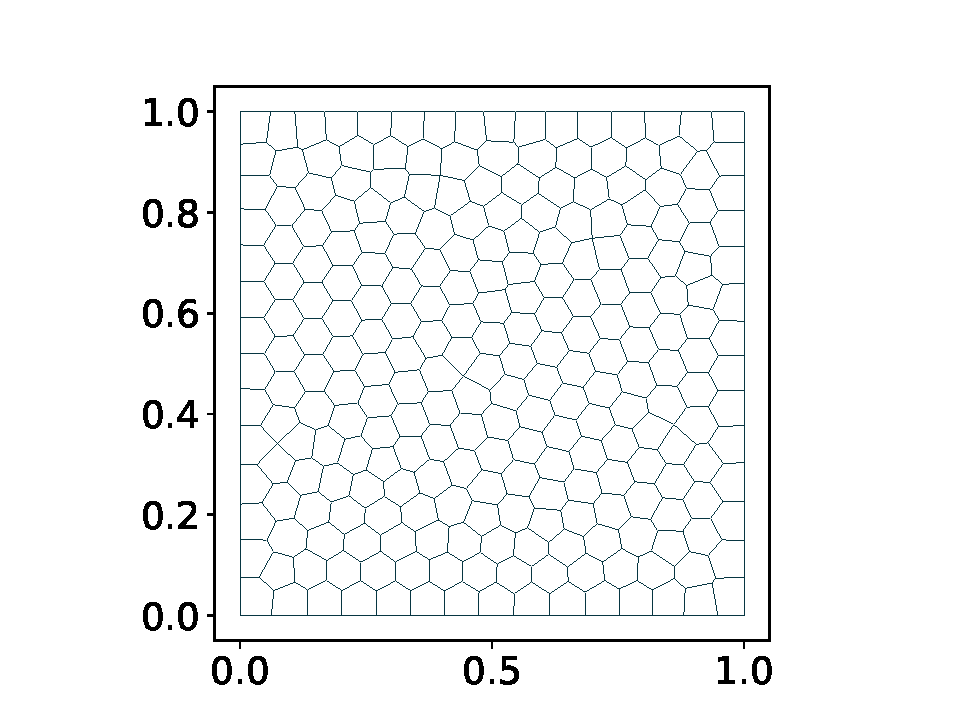
\includegraphics[trim=2.25cm 0.5cm 1cm 0.5cm, clip, width=1.25\textwidth]{meshes/uniform/square_250.pdf}
                    \caption{An example mesh. $N = 250$.}
                \end{figure}
            \end{flushleft}
        \end{column}
    \end{columns}

\end{frame}

	\newpage
    \section{Solving the Poisson Problem}
	Having built a mesh over a polygonal domain, the Poisson problem can be solved by first constructing the problem's matrix $\MA$ and the forcing term $\VB$ as described in \eqref{matrix} and \eqref{forcing}.

The \lstinline{laplacian} function constructs the matrices used for solving the problem and evaluating errors by computing all terms in \eqref{boa} for each element. The resulting matrices are in sparse form.

The \lstinline{forcing} function constructs the forcing term by evaluating \eqref{forcing} and enforces the Dirichlet boundary condition \eqref{dirichlet} through penalization.

\cite{Saad2003} The solution to the matrix equation $\MA \Vector{\upsilon}^k_h = \VB$ is obtained using the \lstinline{BICGSTAB} algorithm, with the \lstinline{GMRES} algorithm used if the first one fails to converge within a fixed number of steps. Both of these iterative algorithms for sparse matrices have been implemented in the \textit{algebra} section of the code.

On adaptively refined meshes, $\kappa(\MA)$ rapidly grows, necessitating the use of a preconditioner within the custom solver \lstinline{lapsolver}.

Let $\MM$ and $(\mathcal{V}_{DG} + \mathcal{S}_{DG})$ be the mass and $DG$ matrices. The $L^2$ and $DG$ errors are then evaluated by first computing the modal coefficients $\Vector{\upsilon}_m$ for the exact solution $u$ and solving $\MM \Vector{u} = \Vector{\upsilon}_m$ using the \lstinline{DB}\footnote{Block diagonal algorithm.} algorithm. Thus, the error vector is $\Vector{e} = \Vector{\upsilon} - \Vector{\upsilon}^k_h$. Hence:

\begin{gather}
    \lVert u - u^k_h \rVert_{\LT(\Omega)} = \sqrt{\Vector{e}^\intercal \MM \Vector{e}}, \\
    \lVert u - u^k_h \rVert_{DG} = \sqrt{\Vector{e}^\intercal (\mathcal{V}_{DG} + \mathcal{S}_{DG}) \Vector{e}},
\end{gather}

Some examples are provided in the following sections.

\newpage
\subsection{A code snippet}

Here's a snippet to illustrate the Poisson solution process from the user's perspective:

\lstinputlisting[style=cpp, firstline=11]{../snippets/poisson.cpp}

	\newpage
    \section{Tests over a Sequence of Uniform Meshes}
	\subsection{Smooth solutions}

Tests over a sequence of uniform meshes have been conducted to verify the algorithm's performance, confirming that:

\begin{gather} \label{trends}
    \lVert u - u^k_h \rVert_{\LT(\Omega)} \approx h^{k + 1}, \\
    \lVert u - u^k_h \rVert_{DG} \approx h^k.
\end{gather}

These results were obtained by selecting a smooth function as the exact solution, such as:

\begin{gather}
    u(x, y) = \sin(2 \pi x) \cos(2 \pi y),
\end{gather}

which leads to:

\begin{gather}
    f(x, y) = -\Delta u(x, y) = 8 \pi^2 \sin(2 \pi x) \cos(2 \pi y),
\end{gather}

with non-homogeneous Dirichlet boundary conditions given by the exact solution itself.

Error trends are presented in the following sections.

\newpage
\subsubsection{Errors}

The following shows the error trends for the $\LT$ and $DG$ errors over sequences of uniform meshes on square and L-shaped domains. The relations presented in \eqref{trends} have been confirmed.

\begin{figure}[!ht]
    % Errors v Size template for TikZ.

\begin{subfigure}[b]{0.45\textwidth}
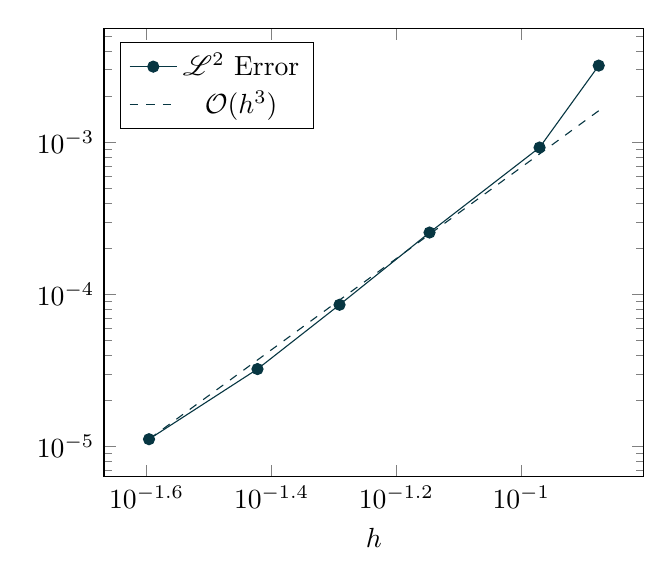
\begin{tikzpicture}
\begin{loglogaxis}[
    xlabel={$h$},
    legend pos=north west,
]

\addplot[solarized-base02, mark=*] coordinates {(0.13307,0.00319602) (0.106989,0.000923928) (0.0713092,0.000254932) (0.0511671,8.53632e-05) (0.0378115,3.22414e-05) (0.0253431,1.11436e-05)};
\addlegendentry{$\LT$ Error}

\addplot[solarized-base02, dashed] coordinates {(0.13307,0.0016131946519815491) (0.0253431,1.11436e-05)};
\addlegendentry{$\mathcal{O}(h^{3})$}

\end{loglogaxis}
\end{tikzpicture}
\end{subfigure}
\hfill
\begin{subfigure}[b]{0.45\textwidth}
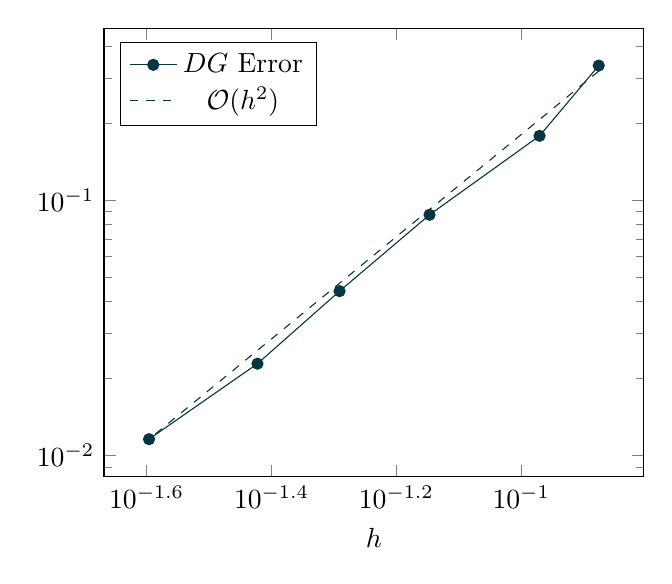
\begin{tikzpicture}
\begin{loglogaxis}[
    xlabel={$h$},
    legend pos=north west,
]

\addplot[solarized-base02, mark=*] coordinates {(0.13307,0.335441) (0.106989,0.178159) (0.0713092,0.087464) (0.0511671,0.0439649) (0.0378115,0.0228686) (0.0253431,0.0115813)};
\addlegendentry{$DG$ Error}

\addplot[solarized-base02, dashed] coordinates {(0.13307,0.3192994356314801) (0.0253431,0.0115813)};
\addlegendentry{$\mathcal{O}(h^{2})$}

\end{loglogaxis}
\end{tikzpicture}
\end{subfigure}
    % Errors v Size template for TikZ.

\begin{subfigure}[b]{0.45\textwidth}
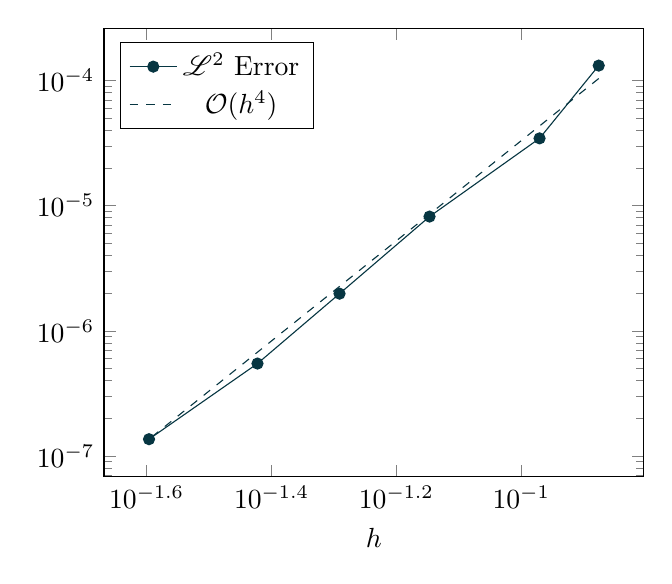
\begin{tikzpicture}
\begin{loglogaxis}[
    xlabel={$h$},
    legend pos=north west,
]

\addplot[solarized-base02, mark=*] coordinates {(0.13307,0.000131393) (0.106989,3.44649e-05) (0.0713092,8.1769e-06) (0.0511671,1.98114e-06) (0.0378115,5.47747e-07) (0.0253431,1.36302e-07)};
\addlegendentry{$\LT$ Error}

\addplot[solarized-base02, dashed] coordinates {(0.13307,0.0001036057614569891) (0.0253431,1.36302e-07)};
\addlegendentry{$\mathcal{O}(h^{4})$}

\end{loglogaxis}
\end{tikzpicture}
\end{subfigure}
\hfill
\begin{subfigure}[b]{0.45\textwidth}
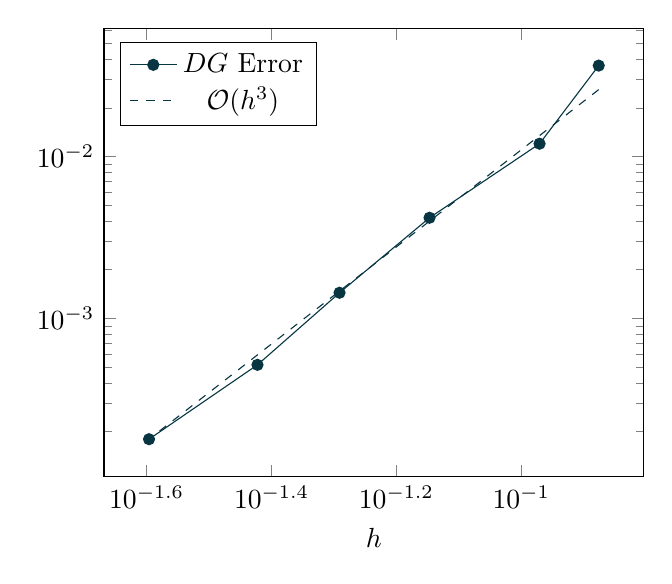
\begin{tikzpicture}
\begin{loglogaxis}[
    xlabel={$h$},
    legend pos=north west,
]

\addplot[solarized-base02, mark=*] coordinates {(0.13307,0.036557) (0.106989,0.0120258) (0.0713092,0.00419264) (0.0511671,0.00144215) (0.0378115,0.000517054) (0.0253431,0.000179452)};
\addlegendentry{$DG$ Error}

\addplot[solarized-base02, dashed] coordinates {(0.13307,0.025978230256595083) (0.0253431,0.000179452)};
\addlegendentry{$\mathcal{O}(h^{3})$}

\end{loglogaxis}
\end{tikzpicture}
\end{subfigure}
    \caption{$\LT$ and $DG$ errors versus mesh size on a sequence of uniform meshes over a square domain. $k = 2$ (top), $k = 3$ (bottom), with $N \in \{125, 250, \dots, 4000\}$.}
\end{figure}

\newpage
\begin{figure}[!ht]
    % Errors v Size template for TikZ.

\begin{subfigure}[b]{0.45\textwidth}
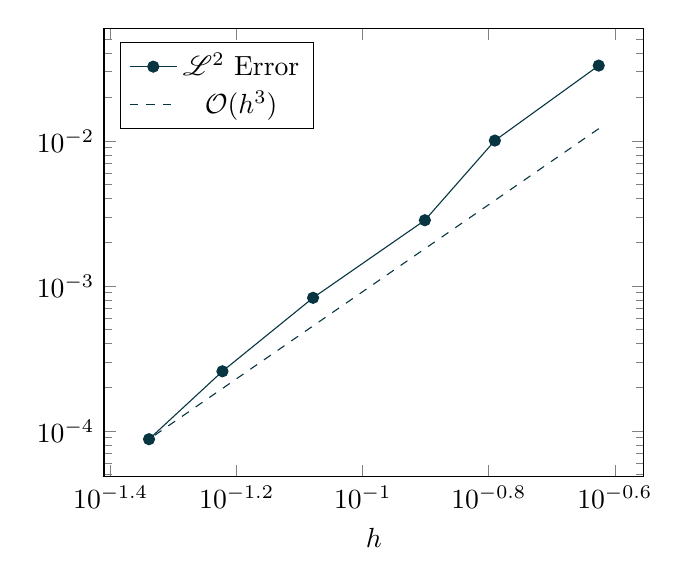
\begin{tikzpicture}
\begin{loglogaxis}[
    xlabel={$h$},
    legend pos=north west,
]

\addplot[solarized-base02, mark=*] coordinates {(0.236846,0.033079) (0.162063,0.0100577) (0.125487,0.00284011) (0.0834066,0.000829064) (0.0598985,0.000258195) (0.0458041,8.78696e-05)};
\addlegendentry{$\LT$ Error}

\addplot[solarized-base02, dashed] coordinates {(0.236846,0.012148530558035811) (0.0458041,8.78696e-05)};
\addlegendentry{$\mathcal{O}(h^{3})$}

\end{loglogaxis}
\end{tikzpicture}
\end{subfigure}
\hfill
\begin{subfigure}[b]{0.45\textwidth}
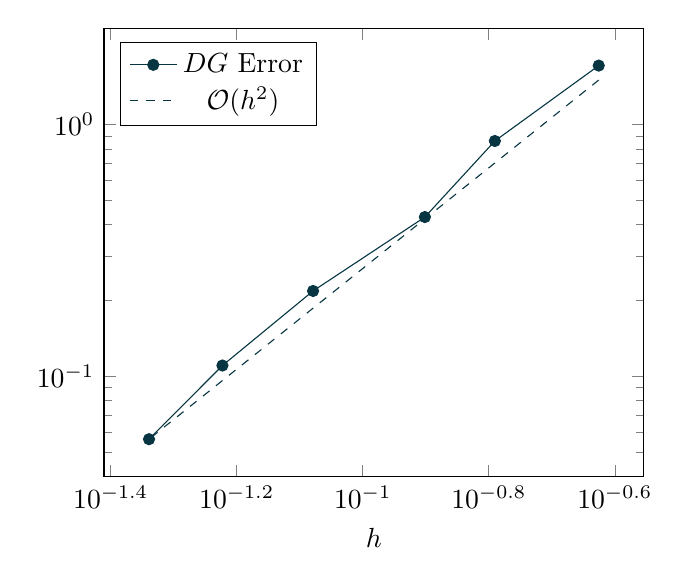
\begin{tikzpicture}
\begin{loglogaxis}[
    xlabel={$h$},
    legend pos=north west,
]

\addplot[solarized-base02, mark=*] coordinates {(0.236846,1.71328) (0.162063,0.859474) (0.125487,0.428497) (0.0834066,0.217901) (0.0598985,0.110162) (0.0458041,0.0561394)};
\addlegendentry{$DG$ Error}

\addplot[solarized-base02, dashed] coordinates {(0.236846,1.501036204482293) (0.0458041,0.0561394)};
\addlegendentry{$\mathcal{O}(h^{2})$}

\end{loglogaxis}
\end{tikzpicture}
\end{subfigure}
    % Errors v Size template for TikZ.

\begin{subfigure}[b]{0.45\textwidth}
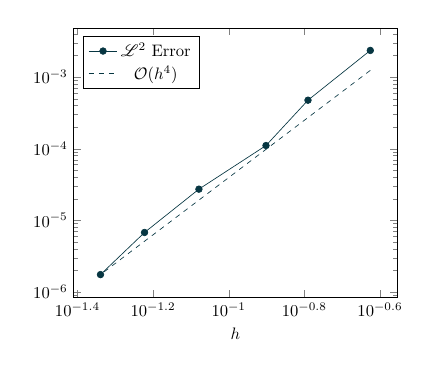
\begin{tikzpicture}[scale=.6]
\begin{loglogaxis}[
    xlabel={$h$},
    legend pos=north west,
]

\addplot[solarized-base02, mark=*] coordinates {(0.236846,0.00236589) (0.162063,0.000476832) (0.125487,0.000110835) (0.0834066,2.72149e-05) (0.0598985,6.75002e-06) (0.0458041,1.74035e-06)};
\addlegendentry{$\LT$ Error}

\addplot[solarized-base02, dashed] coordinates {(0.236846,0.0012441805245544592) (0.0458041,1.74035e-06)};
\addlegendentry{$\mathcal{O}(h^{4})$}

\end{loglogaxis}
\end{tikzpicture}
\end{subfigure}
\hfill
\begin{subfigure}[b]{0.45\textwidth}
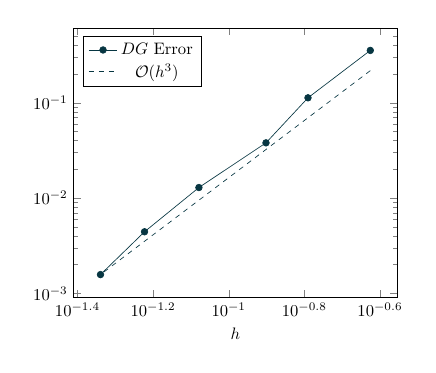
\begin{tikzpicture}[scale=.6]
\begin{loglogaxis}[
    xlabel={$h$},
    legend pos=north west,
]

\addplot[solarized-base02, mark=*] coordinates {(0.236846,0.354304) (0.162063,0.112679) (0.125487,0.0379581) (0.0834066,0.0128848) (0.0598985,0.00442298) (0.0458041,0.0015715)};
\addlegendentry{$DG$ Error}

\addplot[solarized-base02, dashed] coordinates {(0.236846,0.2172698609297559) (0.0458041,0.0015715)};
\addlegendentry{$\mathcal{O}(h^{3})$}

\end{loglogaxis}
\end{tikzpicture}
\end{subfigure}
    \caption{$\LT$ and $DG$ errors versus mesh size on a sequence of uniform meshes over an L-shaped domain. $k = 2$ (top), $k = 3$ (bottom), with $N \in \{125, 250, \dots, 4000\}$.}
\end{figure}

\newpage
\subsubsection{Meshes}

\begin{figure}[!ht]
	\centering
	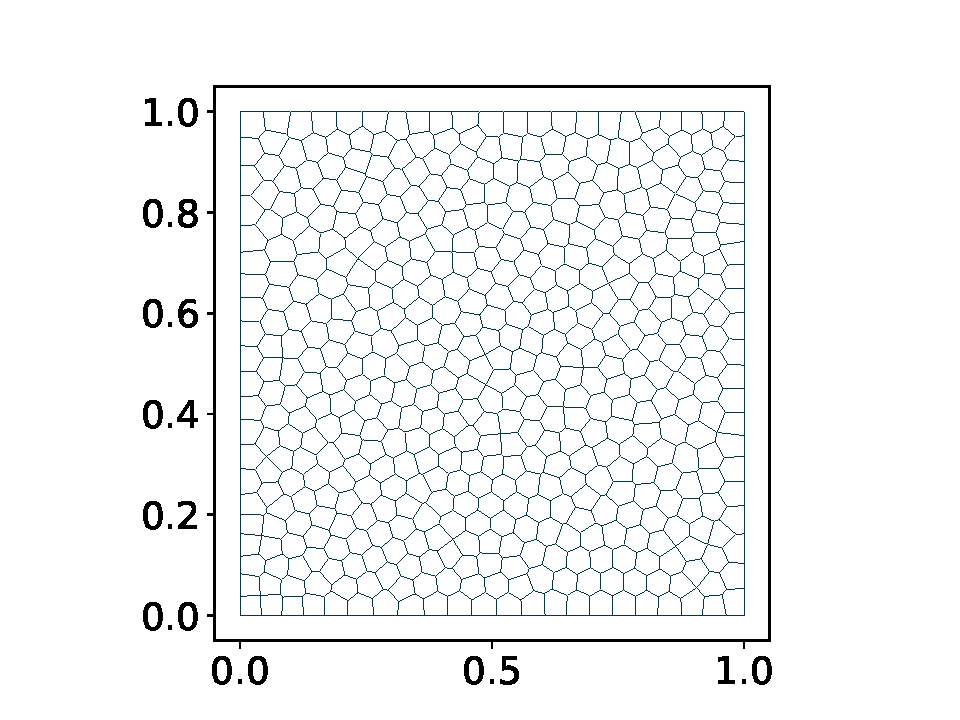
\includegraphics[trim=1cm 0.5cm 1cm 0.5cm, clip, width=0.3\textwidth]{meshes/uniform/square_500.pdf}
	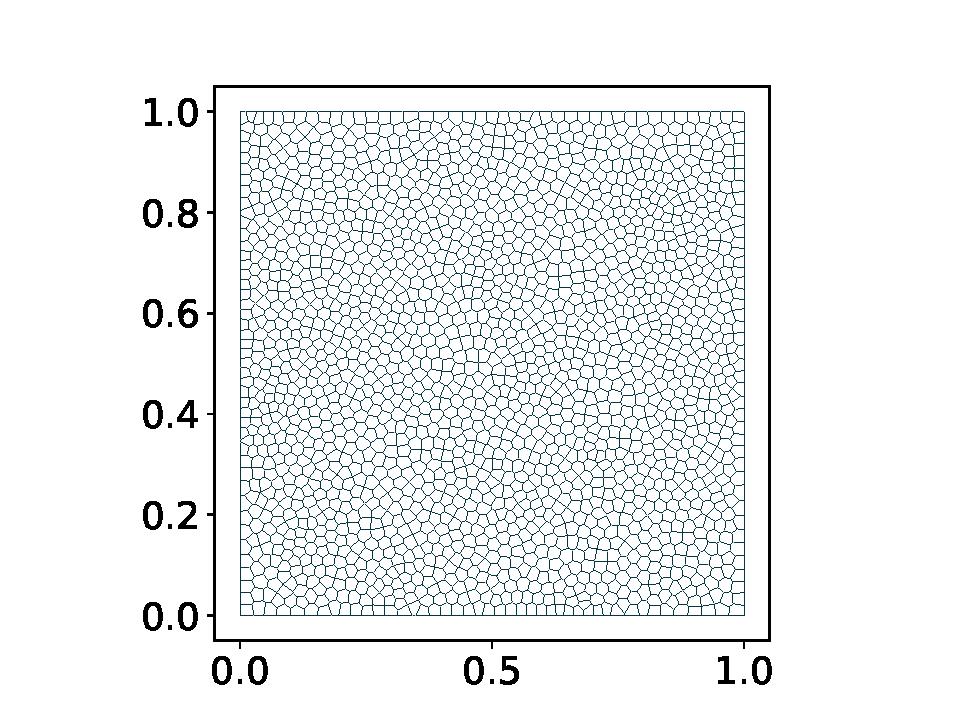
\includegraphics[trim=1cm 0.5cm 1cm 0.5cm, clip, width=0.3\textwidth]{meshes/uniform/square_2000.pdf}
	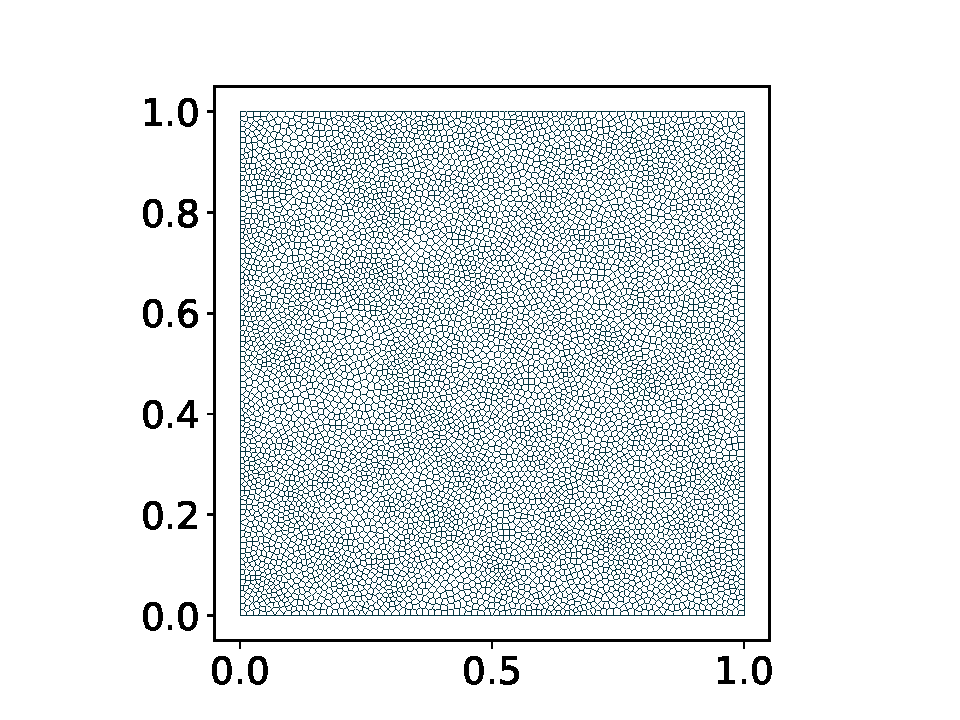
\includegraphics[trim=1cm 0.5cm 1cm 0.5cm, clip, width=0.3\textwidth]{meshes/uniform/square_8000.pdf}
	\caption{Square uniform meshes, with $N \in \{500, 2000, 8000\}$.}
\end{figure}

\begin{figure}[!ht]
	\centering
	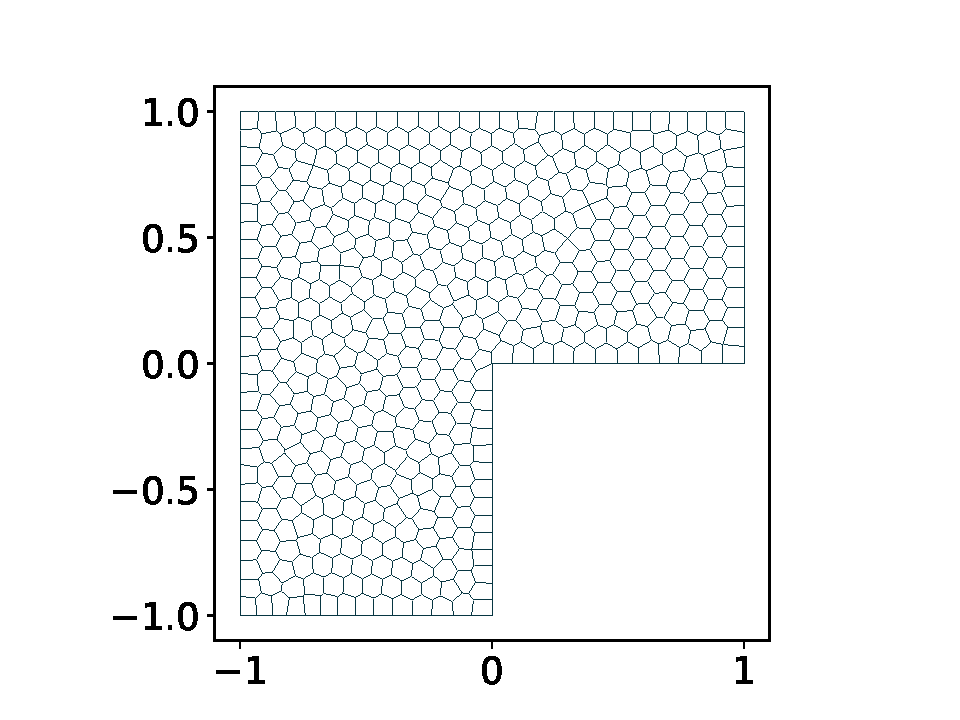
\includegraphics[trim=1cm 0.5cm 1cm 0.5cm, clip, width=0.3\textwidth]{meshes/uniform/lshape_500.pdf}
	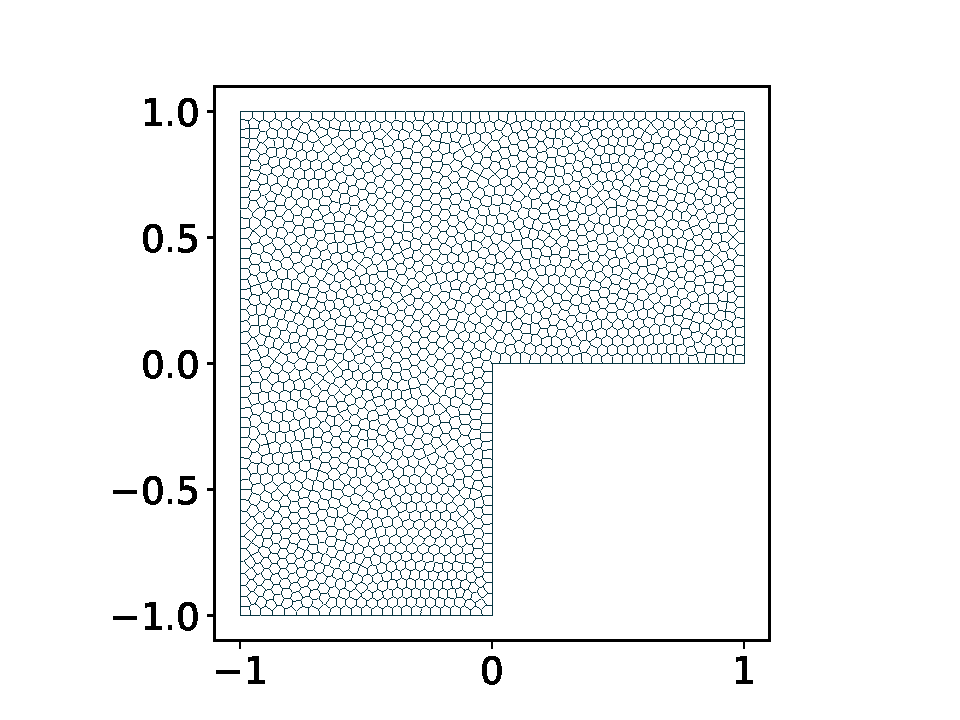
\includegraphics[trim=1cm 0.5cm 1cm 0.5cm, clip, width=0.3\textwidth]{meshes/uniform/lshape_2000.pdf}
	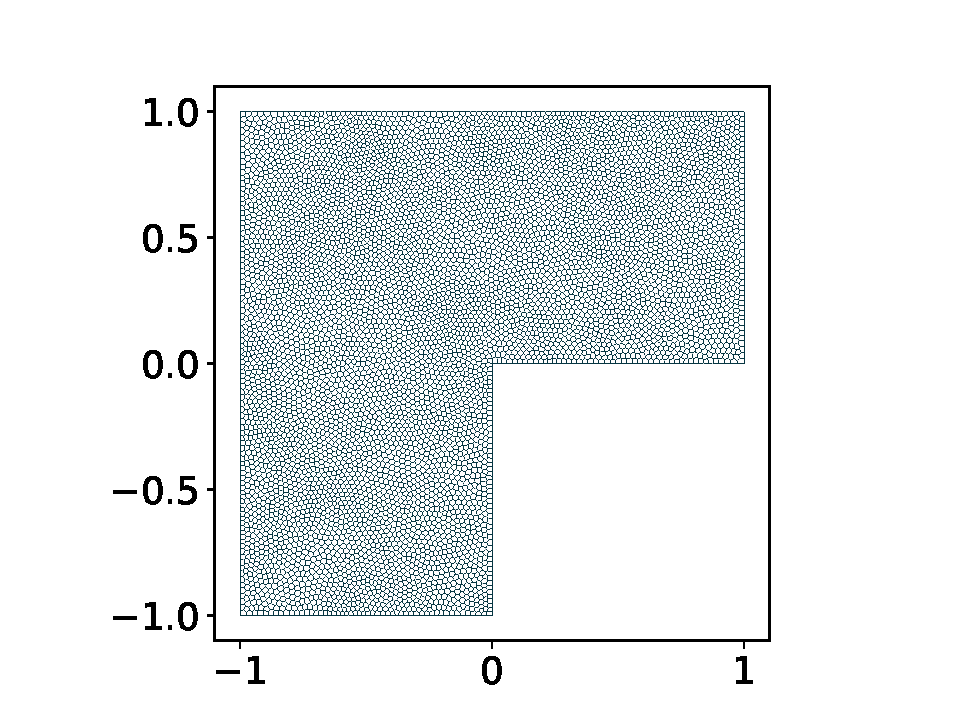
\includegraphics[trim=1cm 0.5cm 1cm 0.5cm, clip, width=0.3\textwidth]{meshes/uniform/lshape_8000.pdf}
	\caption{L-shaped uniform meshes, with $N \in \{500, 2000, 8000\}$.}
\end{figure}

\newpage
\subsection{Low-regularity solutions}

Tests over a sequence of uniform meshes, using low-regularity functions as exact solutions, highlight the need for an adaptive algorithm.

\cite{Antonietti2013} The low-regularity function for the square domain is:

\begin{gather} \label{low-regularity_square}
    u(x, y) = \frac{1 - e^{-100x}}{1 - e^{-100}} \sin(\pi y) (1 - x),
\end{gather}

which exhibits a strong boundary layer along the line $x = 0$.

For the L-shaped domain, the low-regularity function is:

\begin{gather} \label{low-regularity_lshape}
    u(\rho, \theta) = \rho^{2 / 3} \sin\left(\frac{2 \theta}{3}\right),
\end{gather}

where $f = 0$ and $u$ is analytical in $\Omega \setminus \Vector{0}$, but $\grad{u}$ is singular at the origin.

Error trends are discussed in the following sections.

\newpage
\subsubsection{Errors}

Being a smooth function, the low-regularity solution over the square domain achieves the expected convergence rate, albeit at a slower pace.

\begin{figure}[!ht]
    % Errors v Size template for TikZ.

\begin{subfigure}[b]{0.45\textwidth}
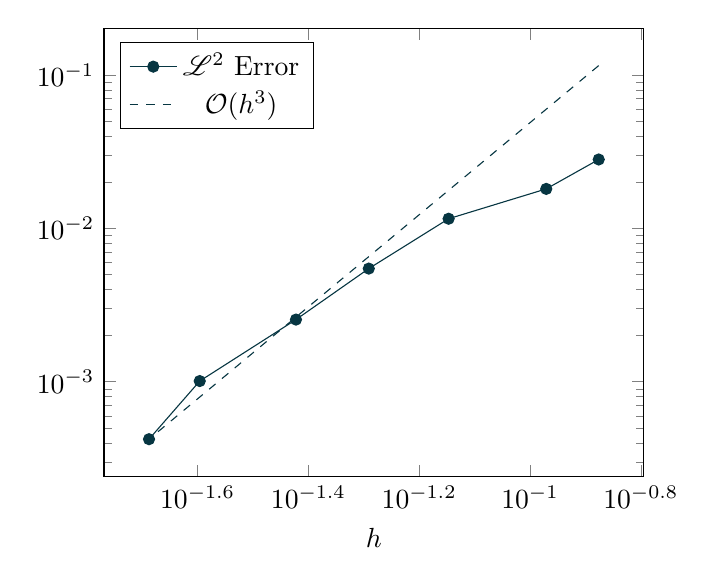
\begin{tikzpicture}
\begin{loglogaxis}[
    xlabel={$h$},
    legend pos=north west,
]

\addplot[solarized-base02, mark=*] coordinates {(0.13307,0.0281162) (0.106989,0.0180826) (0.0713092,0.0115527) (0.0511671,0.00546711) (0.0378115,0.00254289) (0.0253431,0.00101081) (0.0205266,0.000422415)};
\addlegendentry{$\LT$ Error}

\addplot[solarized-base02, dashed] coordinates {(0.13307,0.11508765584587866) (0.0205266,0.000422415)};
\addlegendentry{$\mathcal{O}(h^{3})$}

\end{loglogaxis}
\end{tikzpicture}
\end{subfigure}
\hfill
\begin{subfigure}[b]{0.45\textwidth}
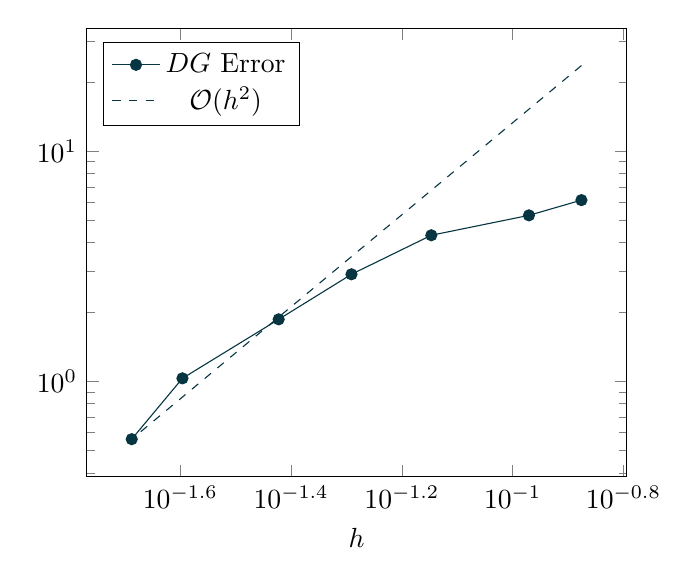
\begin{tikzpicture}
\begin{loglogaxis}[
    xlabel={$h$},
    legend pos=north west,
]

\addplot[solarized-base02, mark=*] coordinates {(0.13307,6.12566) (0.106989,5.25995) (0.0713092,4.30988) (0.0511671,2.91652) (0.0378115,1.85839) (0.0253431,1.02974) (0.0205266,0.5601)};
\addlegendentry{$DG$ Error}

\addplot[solarized-base02, dashed] coordinates {(0.13307,23.539208068455636) (0.0205266,0.5601)};
\addlegendentry{$\mathcal{O}(h^{2})$}

\end{loglogaxis}
\end{tikzpicture}
\end{subfigure}
    % Errors v Size template for TikZ.

\begin{subfigure}[b]{0.45\textwidth}
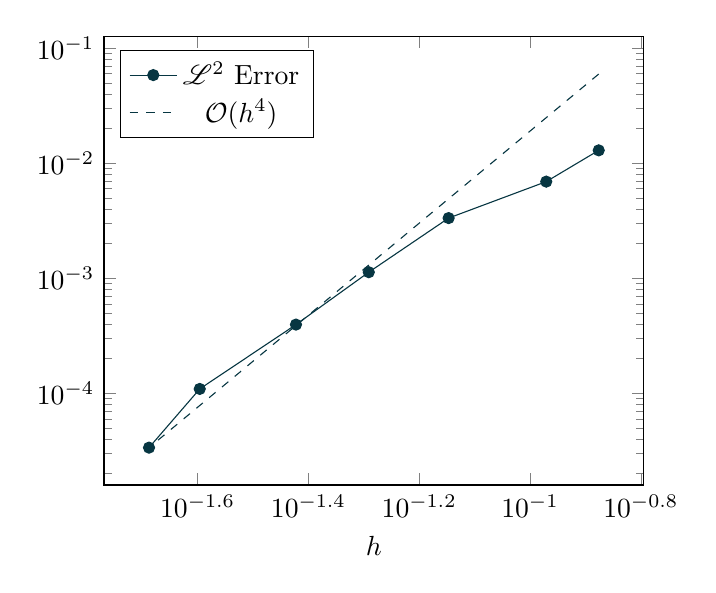
\begin{tikzpicture}
\begin{loglogaxis}[
    xlabel={$h$},
    legend pos=north west,
]

\addplot[solarized-base02, mark=*] coordinates {(0.13307,0.0129373) (0.106989,0.00691892) (0.0713092,0.00333505) (0.0511671,0.0011295) (0.0378115,0.000395856) (0.0253431,0.000109201) (0.0205266,3.37306e-05)};
\addlegendentry{$\LT$ Error}

\addplot[solarized-base02, dashed] coordinates {(0.13307,0.05957672373397235) (0.0205266,3.37306e-05)};
\addlegendentry{$\mathcal{O}(h^{4})$}

\end{loglogaxis}
\end{tikzpicture}
\end{subfigure}
\hfill
\begin{subfigure}[b]{0.45\textwidth}
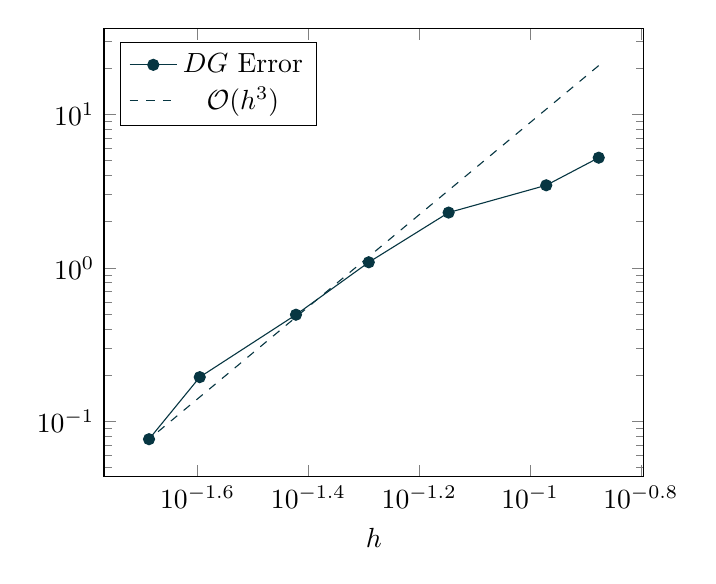
\begin{tikzpicture}
\begin{loglogaxis}[
    xlabel={$h$},
    legend pos=north west,
]

\addplot[solarized-base02, mark=*] coordinates {(0.13307,5.22824) (0.106989,3.45593) (0.0713092,2.29411) (0.0511671,1.08811) (0.0378115,0.495229) (0.0253431,0.194102) (0.0205266,0.0764724)};
\addlegendentry{$DG$ Error}

\addplot[solarized-base02, dashed] coordinates {(0.13307,20.83503013128883) (0.0205266,0.0764724)};
\addlegendentry{$\mathcal{O}(h^{3})$}

\end{loglogaxis}
\end{tikzpicture}
\end{subfigure}
    \caption{$\LT$ and $DG$ errors versus mesh size on a sequence of uniform meshes over a square domain. $k = 2$ (top), $k = 3$ (bottom), with $N \in \{125, 250, \dots, 8000\}$.}
\end{figure}

\newpage

Due to its nature, the low-regularity solution on the L-shaped domain does not reach the expected convergence rate. The expected convergence rate, given its Sobolev regularity, is:

\begin{gather}
    \lVert u - u^k_h \rVert_{DG} \approx h^{2/3}.
\end{gather}

\begin{figure}[!ht]
    % Errors v Size template for TikZ.

\begin{subfigure}[b]{0.45\textwidth}
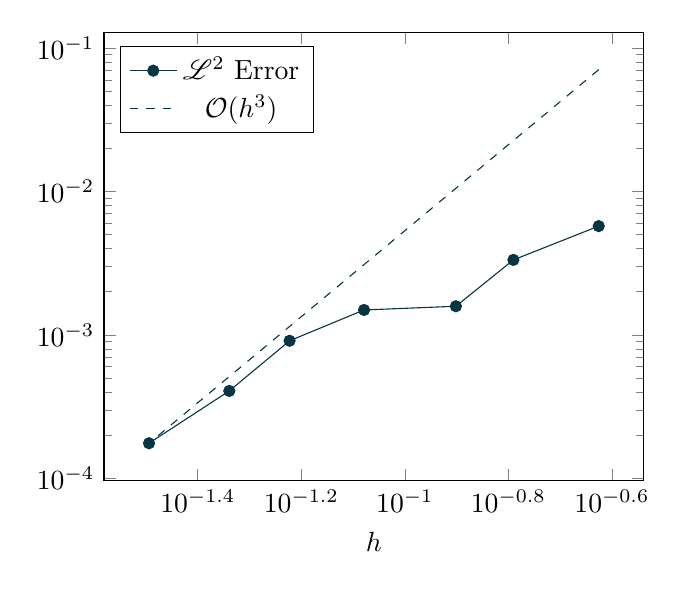
\begin{tikzpicture}
\begin{loglogaxis}[
    xlabel={$h$},
    legend pos=north west,
]

\addplot[solarized-base02, mark=*] coordinates {(0.236846,0.00573887) (0.162063,0.00333593) (0.125487,0.00158497) (0.0834066,0.00149286) (0.0598985,0.000910291) (0.0458041,0.000406813) (0.0320544,0.000175592)};
\addlegendentry{$\LT$ Error}

\addplot[solarized-base02, dashed] coordinates {(0.236846,0.07083370080315939) (0.0320544,0.000175592)};
\addlegendentry{$\mathcal{O}(h^{3})$}

\end{loglogaxis}
\end{tikzpicture}
\end{subfigure}
\hfill
\begin{subfigure}[b]{0.45\textwidth}
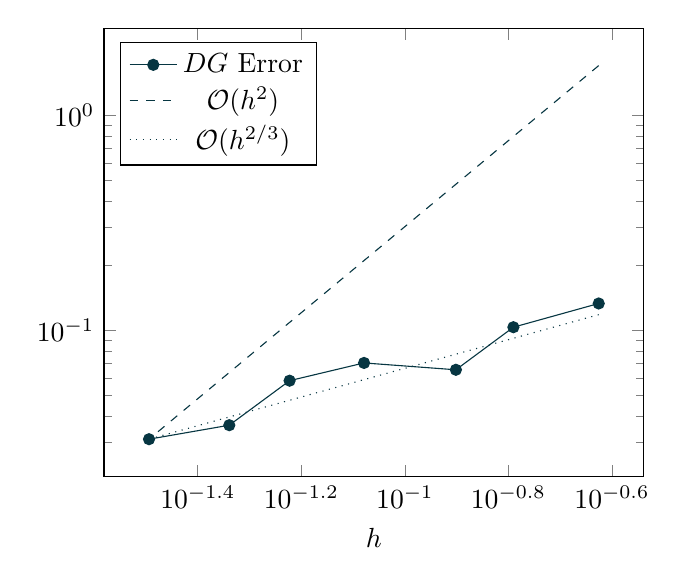
\begin{tikzpicture}
\begin{loglogaxis}[
    xlabel={$h$},
    legend pos=north west,
]

\addplot[solarized-base02, mark=*] coordinates {(0.236846,0.13327) (0.162063,0.103364) (0.125487,0.0655287) (0.0834066,0.0705169) (0.0598985,0.0583046) (0.0458041,0.0362069) (0.0320544,0.0311668)};
\addlegendentry{$DG$ Error}

\addplot[solarized-base02, dashed] coordinates {(0.236846,1.7015668612169044) (0.0320544,0.0311668)};
\addlegendentry{$\mathcal{O}(h^{2})$}

\addplot[solarized-base02, dotted] coordinates {(0.236846,0.11823457166349788) (0.0320544,0.0311668)};
\addlegendentry{$\mathcal{O}(h^{2/3})$}

\end{loglogaxis}
\end{tikzpicture}
\end{subfigure}
    % Errors v Size template for TikZ.

\begin{subfigure}[b]{0.45\textwidth}
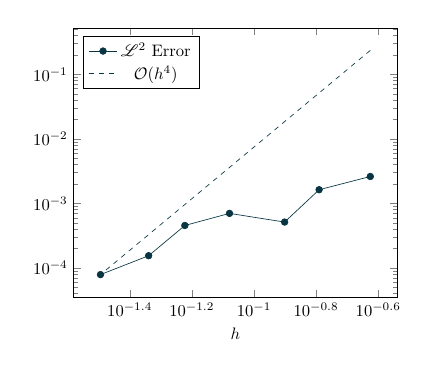
\begin{tikzpicture}[scale=.6]
\begin{loglogaxis}[
    xlabel={$h$},
    legend pos=north west,
]

\addplot[solarized-base02, mark=*] coordinates {(0.236846,0.00261101) (0.162063,0.00162784) (0.125487,0.000513351) (0.0834066,0.000699775) (0.0598985,0.000454435) (0.0458041,0.000154545) (0.0320544,7.87786e-05)};
\addlegendentry{$\LT$ Error}

\addplot[solarized-base02, dashed] coordinates {(0.236846,0.23481285454935658) (0.0320544,7.87786e-05)};
\addlegendentry{$\mathcal{O}(h^{4})$}

\end{loglogaxis}
\end{tikzpicture}
\end{subfigure}
\hfill
\begin{subfigure}[b]{0.45\textwidth}
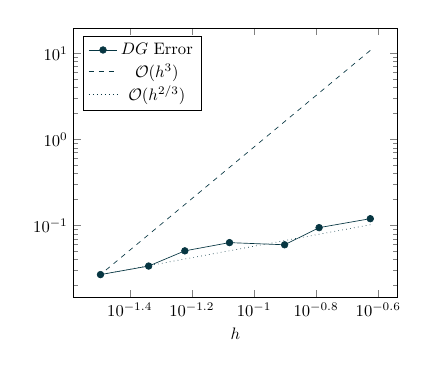
\begin{tikzpicture}[scale=.6]
\begin{loglogaxis}[
    xlabel={$h$},
    legend pos=north west,
]

\addplot[solarized-base02, mark=*] coordinates {(0.236846,0.119546) (0.162063,0.0940845) (0.125487,0.0594576) (0.0834066,0.0630073) (0.0598985,0.0505441) (0.0458041,0.0336456) (0.0320544,0.0267768)};
\addlegendentry{$DG$ Error}

\addplot[solarized-base02, dashed] coordinates {(0.236846,10.801744041106874) (0.0320544,0.0267768)};
\addlegendentry{$\mathcal{O}(h^{3})$}

\addplot[solarized-base02, dotted] coordinates {(0.236846,0.10158063960750381) (0.0320544,0.0267768)};
\addlegendentry{$\mathcal{O}(h^{2/3})$}

\end{loglogaxis}
\end{tikzpicture}
\end{subfigure}
    \caption{$\LT$ and $DG$ errors versus mesh size on a sequence of uniform meshes over an L-shaped domain. $k = 2$ (top), $k = 3$ (bottom), with $N \in \{125, 250, \dots, 8000\}$.}
\end{figure}

	\newpage
    \section{Implementing \textit{h-Adaptivity}}
	\subsection{A priori error estimates}

The need for \textit{h-adaptivity} arises from the inefficiency encountered when solving the Poisson problem over sequences of uniform meshes, especially when dealing with low-regularity exact solutions such as \eqref{low-regularity_square} and \eqref{low-regularity_lshape}.

To implement \textit{h-adaptivity}, the first step is to evaluate the $\LT$ error on each element and then refine the element with the highest error according to a specific refinement strategy.

The strategy of choice can be outlined as follows:

\begin{enumerate}
    \item For polygons with $N_e \leq 4$, the refiner adds a single node at the polygon's centroid and then connects each edge's midpoint to this new node, creating $N_e$ new quadrilaterals.
    \item For polygons with $N_e > 4$, the refiner adds $N_e$ new nodes at the midpoints of the segments connecting the polygon's centroid to the midpoints of its edges. The refiner then connects these points to form quadrilaterals along the polygon's edges and creates a new smaller polygon by connecting all the new internal nodes.
\end{enumerate}

Refinement occurs by setting a refinement percentage and marking all elements where the local error exceeds that percentage of the highest error. Let $\sigma$ be this percentage, the elements $K$ to be refined are those such that:

\begin{gather}
	\eta_K > \sigma \eta_{M},
\end{gather}

where $\eta_K$ is the local error and $\eta_M$ is the highest error.

Error trends and refined meshes are presented in the following sections. For all examples shown, $\sigma = 75\%$.

\newpage
\subsubsection{Errors}

The following plots demonstrate that the adaptive approach (blue) significantly outperforms uniform refinement (black) when handling these low-regularity solutions\footnote{$N \in \{125, 250, \dots, 8000\}$ for the uniform meshes.}.

\begin{figure}[!ht]
	\begin{subfigure}[b]{0.45\textwidth}
		% Errors v DOFs template for TikZ.

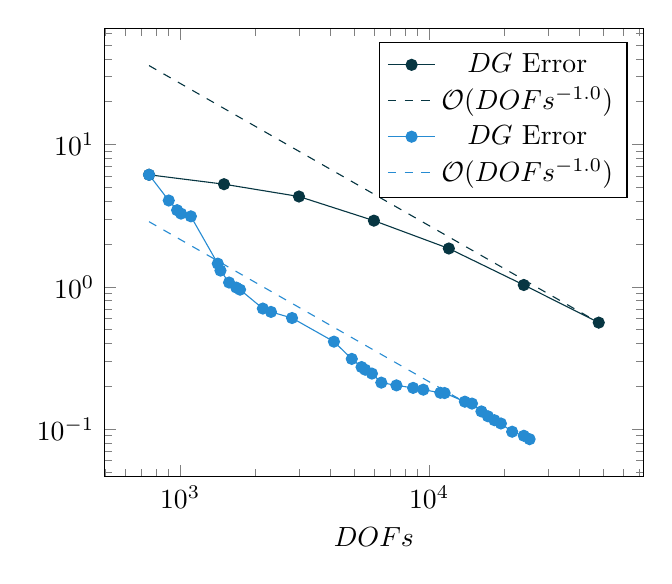
\begin{tikzpicture}
\begin{loglogaxis}[
    xlabel={$DOFs$},
    legend pos=north east,
]

\addplot[solarized-base02, mark=*] coordinates {(750,6.12566) (1500,5.25995) (3000,4.30988) (6000,2.91652) (12000,1.85839) (24000,1.02974) (48000,0.5601)};
\addlegendentry{$DG$ Error}

\addplot[solarized-base02, dashed] coordinates {(750,35.8464) (48000,0.5601)};
\addlegendentry{$\mathcal{O}(DOFs^{-1.0})$}

\addplot[\accentcolor, mark=*] coordinates {(750,6.12566) (900,4.03955) (972,3.45362) (1008,3.26799) (1104,3.12636) (1416,1.45431) (1452,1.30003) (1572,1.0716) (1680,0.987916) (1740,0.954643) (2148,0.70325) (2316,0.666102) (2814,0.603387) (4146,0.411693) (4890,0.311397) (5352,0.272847) (5532,0.261592) (5892,0.245583) (6426,0.212127) (7392,0.202913) (8622,0.194848) (9474,0.189286) (11094,0.180045) (11538,0.179227) (13914,0.155865) (14862,0.151127) (16218,0.133144) (17226,0.123047) (18294,0.11549) (19422,0.109519) (21546,0.0958461) (24006,0.0897779) (25320,0.0849597)};
\addlegendentry{$DG$ Error}

\addplot[\accentcolor, dashed] coordinates {(750,2.868239472) (25320,0.0849597)};
\addlegendentry{$\mathcal{O}(DOFs^{-1.0})$}

\end{loglogaxis}
\end{tikzpicture}
	\end{subfigure}
	\hfill
	\begin{subfigure}[b]{0.45\textwidth}
		% Errors v DOFs template for TikZ.

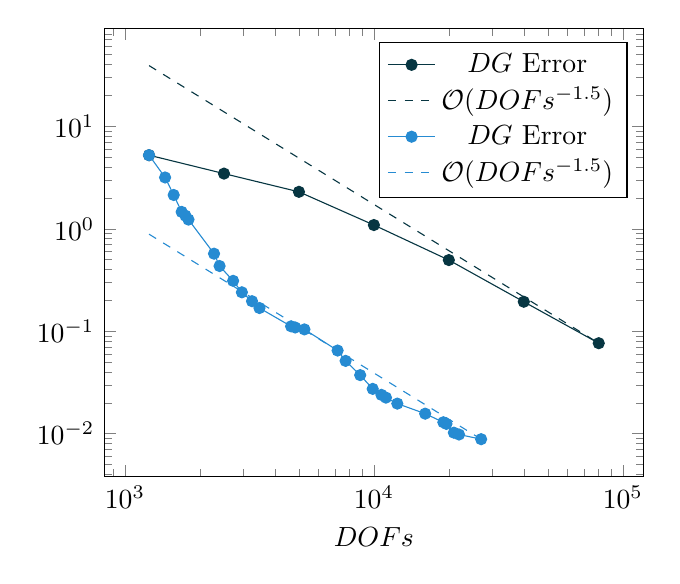
\begin{tikzpicture}
\begin{loglogaxis}[
    xlabel={$DOFs$},
    legend pos=north east,
]

\addplot[solarized-base02, mark=*] coordinates {(1250,5.22824) (2500,3.45593) (5000,2.29411) (10000,1.08811) (20000,0.495229) (40000,0.194102) (80000,0.0764724)};
\addlegendentry{$DG$ Error}

\addplot[solarized-base02, dashed] coordinates {(1250,39.1538688) (80000,0.0764724)};
\addlegendentry{$\mathcal{O}(DOFs^{-1.5})$}

\addplot[\accentcolor, mark=*] coordinates {(1250,5.22824) (1450,3.16847) (1570,2.13764) (1690,1.46207) (1750,1.34315) (1800,1.22937) (2280,0.571535) (2400,0.433165) (2720,0.310514) (2950,0.239953) (3240,0.196515) (3470,0.168581) (4650,0.111757) (4830,0.108861) (5260,0.104274) (7150,0.0648557) (7700,0.0513934) (8810,0.0373304) (9890,0.0273954) (10720,0.0239574) (11180,0.0225082) (12420,0.0196702) (16070,0.0156938) (19010,0.0129343) (19560,0.0124709) (20950,0.0102387) (21970,0.00982763) (26960,0.00884522)};
\addlegendentry{$DG$ Error}

\addplot[\accentcolor, dashed] coordinates {(1250,0.8859790477668384) (26960,0.00884522)};
\addlegendentry{$\mathcal{O}(DOFs^{-1.5})$}

\end{loglogaxis}
\end{tikzpicture}
	\end{subfigure}
    \caption{$DG$ errors versus $DOFs$ comparison between adaptively refined meshes and a sequence of uniform meshes over a square domain. $k = 2$ (left) and $k = 3$ (right).}
\end{figure}

\begin{figure}[!ht]
	\begin{subfigure}[b]{0.45\textwidth}
		% Errors v DOFs template for TikZ.

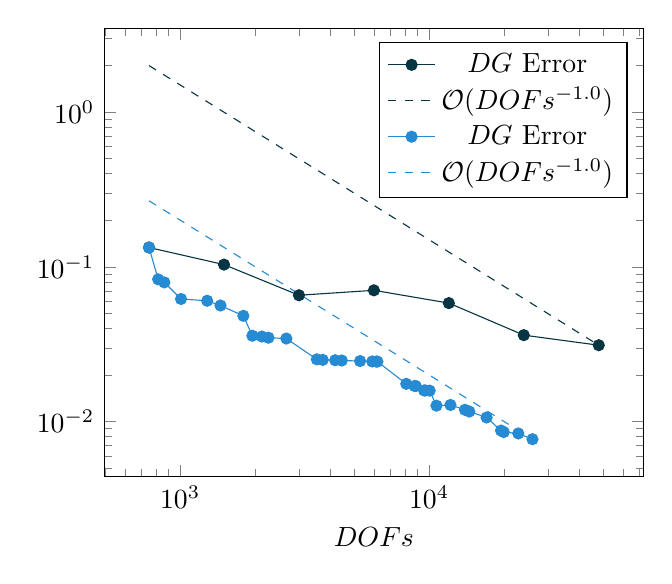
\begin{tikzpicture}
\begin{loglogaxis}[
    xlabel={$DOFs$},
    legend pos=north east,
]

\addplot[solarized-base02, mark=*] coordinates {(750,0.13327) (1500,0.103364) (3000,0.0655286) (6000,0.0705169) (12000,0.0583046) (24000,0.0362069) (48000,0.0311668)};
\addlegendentry{$DG$ Error}

\addplot[solarized-base02, dashed] coordinates {(750,1.9946752) (48000,0.0311668)};
\addlegendentry{$\mathcal{O}(DOFs^{-1.0})$}

\addplot[\accentcolor, mark=*] coordinates {(750,0.13327) (816,0.0830244) (864,0.0793426) (1008,0.0619878) (1284,0.0603523) (1452,0.0562495) (1794,0.0482533) (1950,0.0358904) (2130,0.0354704) (2262,0.0348557) (2670,0.0344147) (3540,0.0252647) (3738,0.0250711) (4194,0.0249254) (4458,0.0248335) (5280,0.0246302) (5910,0.0244758) (6132,0.0244387) (6198,0.0244288) (8094,0.0175423) (8742,0.0169922) (8838,0.0169865) (9546,0.015904) (9660,0.015896) (10050,0.015861) (10698,0.0126811) (12180,0.0128159) (13926,0.0119234) (14502,0.0116229) (17016,0.0106359) (19446,0.00875964) (19938,0.00856267) (22806,0.00838982) (26004,0.00770473)};
\addlegendentry{$DG$ Error}

\addplot[\accentcolor, dashed] coordinates {(750,0.26713839856000005) (26004,0.00770473)};
\addlegendentry{$\mathcal{O}(DOFs^{-1.0})$}

\end{loglogaxis}
\end{tikzpicture}
	\end{subfigure}
	\hfill
	\begin{subfigure}[b]{0.45\textwidth}
		% Errors v DOFs template for TikZ.

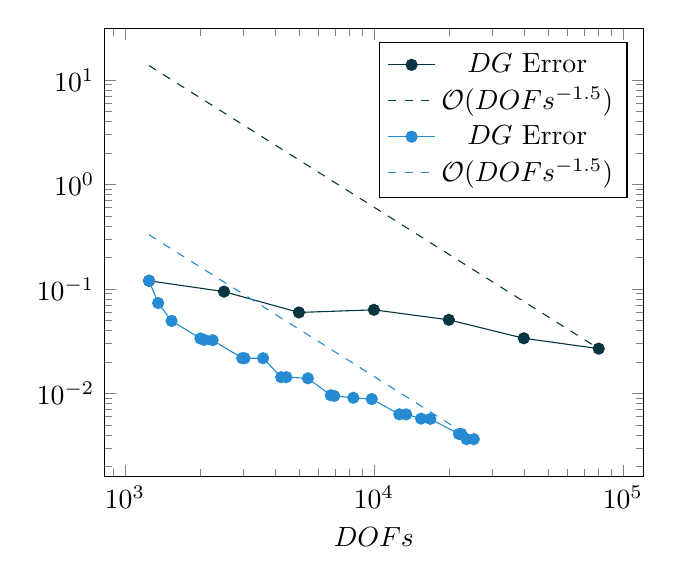
\begin{tikzpicture}
\begin{loglogaxis}[
    xlabel={$DOFs$},
    legend pos=north east,
]

\addplot[solarized-base02, mark=*] coordinates {(1250,0.119546) (2500,0.0940843) (5000,0.0594572) (10000,0.0630071) (20000,0.050544) (40000,0.0336455) (80000,0.0267768)};
\addlegendentry{$DG$ Error}

\addplot[solarized-base02, dashed] coordinates {(1250,13.7097216) (80000,0.0267768)};
\addlegendentry{$\mathcal{O}(DOFs^{-1.5})$}

\addplot[\accentcolor, mark=*] coordinates {(1250,0.119546) (1360,0.0730976) (1540,0.0493759) (2010,0.0335623) (2080,0.0325106) (2250,0.0322421) (2960,0.0217044) (3020,0.0216543) (3590,0.0216774) (4240,0.0142896) (4450,0.0142875) (5430,0.0139307) (6710,0.009591) (6930,0.0094454) (8270,0.00907011) (9800,0.00881814) (12650,0.00629972) (13480,0.00629107) (15470,0.00572756) (16850,0.00569782) (21960,0.00407968) (22460,0.00407912) (23570,0.00364227) (25190,0.00363907)};
\addlegendentry{$DG$ Error}

\addplot[\accentcolor, dashed] coordinates {(1250,0.3292059237674489) (25190,0.00363907)};
\addlegendentry{$\mathcal{O}(DOFs^{-1.5})$}

\end{loglogaxis}
\end{tikzpicture}
	\end{subfigure}
    \caption{$DG$ errors versus $DOFs$ comparison between adaptively refined meshes and a sequence of uniform meshes over an L-shaped domain. $k = 2$ (left) and $k = 3$ (right).}
\end{figure}

\newpage

Due to the nature of the low-regularity solutions, it may be worth considering adaptive refinement based on local $\HO$ errors rather than $\LT$ errors. The following plots show improved results, particularly for the L-shaped domain.

\begin{figure}[!ht]
	\begin{subfigure}[b]{0.45\textwidth}
		% Errors v DOFs template for TikZ.

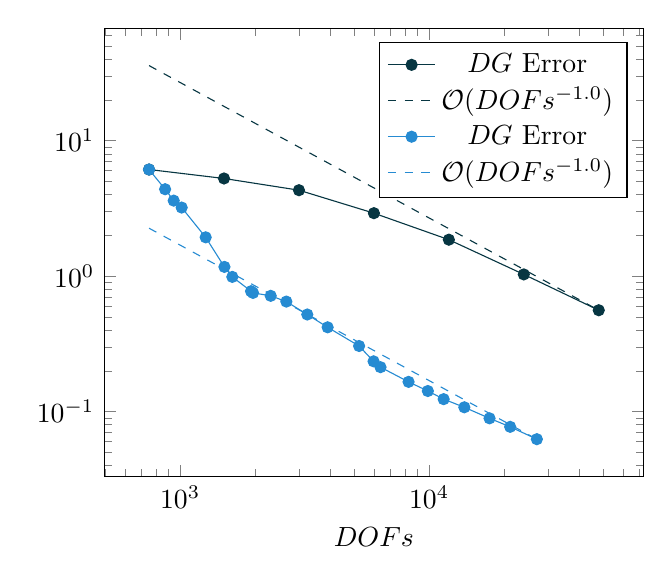
\begin{tikzpicture}
\begin{loglogaxis}[
    xlabel={$DOFs$},
    legend pos=north east,
]

\addplot[solarized-base02, mark=*] coordinates {(750,6.12566) (1500,5.25995) (3000,4.30988) (6000,2.91652) (12000,1.85839) (24000,1.02974) (48000,0.5601)};
\addlegendentry{$DG$ Error}

\addplot[solarized-base02, dashed] coordinates {(750,35.8464) (48000,0.5601)};
\addlegendentry{$\mathcal{O}(DOFs^{-1.0})$}

\addplot[\accentcolor, mark=*] coordinates {(750,6.12566) (870,4.38193) (942,3.60957) (1014,3.20899) (1266,1.93506) (1506,1.16987) (1620,0.987314) (1926,0.773812) (1962,0.752143) (2310,0.715501) (2670,0.648814) (3240,0.520831) (3912,0.419024) (5232,0.304942) (5982,0.234997) (6378,0.212735) (8268,0.165754) (9882,0.141861) (11436,0.123541) (13848,0.107573) (17484,0.0891911) (21156,0.0771805) (27078,0.0625627)};
\addlegendentry{$DG$ Error}

\addplot[\accentcolor, dashed] coordinates {(750,2.2587637207999998) (27078,0.0625627)};
\addlegendentry{$\mathcal{O}(DOFs^{-1.0})$}

\end{loglogaxis}
\end{tikzpicture}
	\end{subfigure}
	\hfill
	\begin{subfigure}[b]{0.45\textwidth}
		% Errors v DOFs template for TikZ.

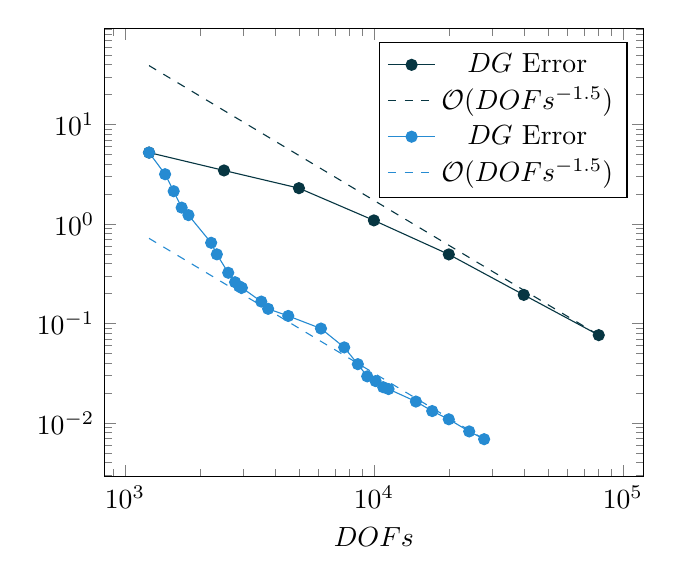
\begin{tikzpicture}
\begin{loglogaxis}[
    xlabel={$DOFs$},
    legend pos=north east,
]

\addplot[solarized-base02, mark=*] coordinates {(1250,5.22824) (2500,3.45593) (5000,2.29411) (10000,1.08811) (20000,0.495229) (40000,0.194102) (80000,0.0764724)};
\addlegendentry{$DG$ Error}

\addplot[solarized-base02, dashed] coordinates {(1250,39.1538688) (80000,0.0764724)};
\addlegendentry{$\mathcal{O}(DOFs^{-1.5})$}

\addplot[\accentcolor, mark=*] coordinates {(1250,5.22824) (1450,3.16847) (1570,2.13764) (1690,1.46207) (1800,1.22937) (2220,0.648223) (2340,0.495982) (2600,0.323852) (2770,0.260152) (2880,0.236183) (2950,0.22874) (3530,0.166199) (3760,0.140521) (4530,0.119187) (6130,0.089056) (7600,0.0575574) (8620,0.0390489) (9400,0.0294453) (10160,0.0263927) (10900,0.0229053) (11450,0.0219544) (14750,0.0164373) (17150,0.0131901) (19990,0.0109056) (24140,0.00823295) (27720,0.00688026)};
\addlegendentry{$DG$ Error}

\addplot[\accentcolor, dashed] coordinates {(1250,0.7185047930727512) (27720,0.00688026)};
\addlegendentry{$\mathcal{O}(DOFs^{-1.5})$}

\end{loglogaxis}
\end{tikzpicture}
	\end{subfigure}
    \caption{$DG$ errors versus $DOFs$ comparison between adaptively refined meshes and a sequence of uniform meshes over a square domain. $k = 2$ (left) and $k = 3$ (right).}
\end{figure}

\begin{figure}[!ht]
	\begin{subfigure}[b]{0.45\textwidth}
		% Errors v DOFs template for TikZ.

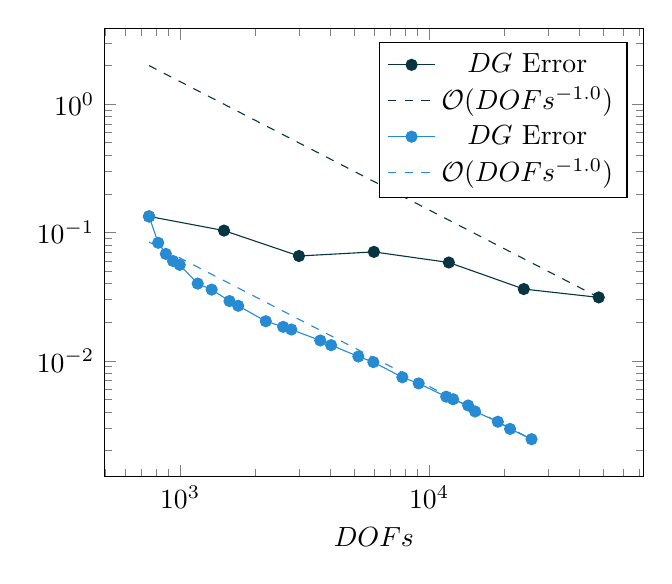
\begin{tikzpicture}
\begin{loglogaxis}[
    xlabel={$DOFs$},
    legend pos=north east,
]

\addplot[solarized-base02, mark=*] coordinates {(750,0.13327) (1500,0.103364) (3000,0.0655286) (6000,0.0705169) (12000,0.0583046) (24000,0.0362069) (48000,0.0311668)};
\addlegendentry{$DG$ Error}

\addplot[solarized-base02, dashed] coordinates {(750,1.9946752) (48000,0.0311668)};
\addlegendentry{$\mathcal{O}(DOFs^{-1.0})$}

\addplot[\accentcolor, mark=*] coordinates {(750,0.13327) (816,0.0830244) (876,0.0680097) (936,0.0598727) (996,0.0559014) (1176,0.039932) (1338,0.0358411) (1578,0.0291867) (1710,0.0268234) (2208,0.0203268) (2592,0.0183746) (2796,0.0175187) (3654,0.0143896) (4038,0.0132366) (5196,0.0107976) (5970,0.00976556) (7806,0.00743953) (9078,0.00666211) (11712,0.00525048) (12480,0.00501671) (14346,0.00448473) (15294,0.00402922) (18876,0.00335053) (21138,0.00294547) (25782,0.00244963)};
\addlegendentry{$DG$ Error}

\addplot[\accentcolor, dashed] coordinates {(750,0.08420848087999999) (25782,0.00244963)};
\addlegendentry{$\mathcal{O}(DOFs^{-1.0})$}

\end{loglogaxis}
\end{tikzpicture}
	\end{subfigure}
	\hfill
	\begin{subfigure}[b]{0.45\textwidth}
		% Errors v DOFs template for TikZ.

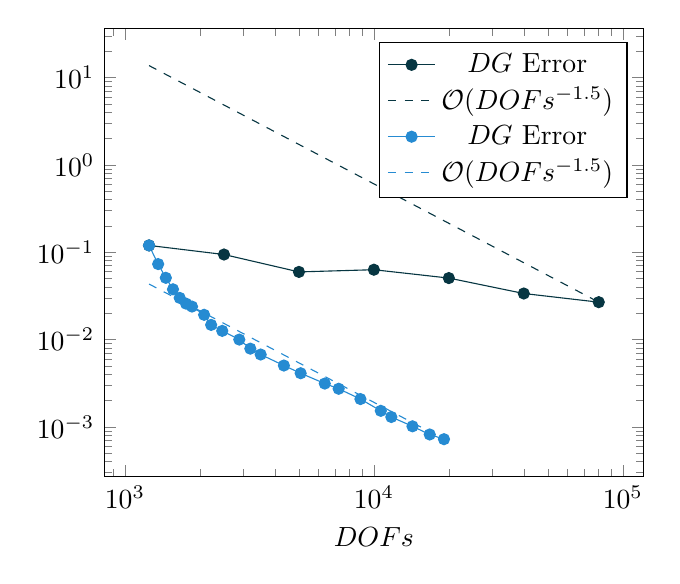
\begin{tikzpicture}
\begin{loglogaxis}[
    xlabel={$DOFs$},
    legend pos=north east,
]

\addplot[solarized-base02, mark=*] coordinates {(1250,0.119546) (2500,0.0940843) (5000,0.0594572) (10000,0.0630071) (20000,0.050544) (40000,0.0336455) (80000,0.0267768)};
\addlegendentry{$DG$ Error}

\addplot[solarized-base02, dashed] coordinates {(1250,13.7097216) (80000,0.0267768)};
\addlegendentry{$\mathcal{O}(DOFs^{-1.5})$}

\addplot[\accentcolor, mark=*] coordinates {(1250,0.119546) (1360,0.0730976) (1460,0.0508708) (1560,0.0375773) (1660,0.0299764) (1760,0.0257653) (1860,0.0238484) (2080,0.0191889) (2220,0.0147015) (2460,0.0125616) (2880,0.00998454) (3190,0.00786125) (3510,0.00673439) (4350,0.0050375) (5080,0.00411082) (6350,0.00313077) (7220,0.00272903) (8830,0.00208062) (10660,0.0015255) (11750,0.00129659) (14290,0.00101426) (16760,0.000817683) (19120,0.00072222)};
\addlegendentry{$DG$ Error}

\addplot[\accentcolor, dashed] coordinates {(1250,0.04320523018854778) (19120,0.00072222)};
\addlegendentry{$\mathcal{O}(DOFs^{-1.5})$}

\end{loglogaxis}
\end{tikzpicture} % Incomplete.
	\end{subfigure}
    \caption{$DG$ errors versus $DOFs$ comparison between adaptively refined meshes and a sequence of uniform meshes over an L-shaped domain. $k = 2$ (left) and $k = 3$ (right).}
\end{figure}

\newpage
\subsubsection{Meshes}

Due to localized errors, the meshes are refined in areas where the error is greatest, thereby minimizing the number of degrees of freedom in regions where the solution is already well-approximated.

\begin{figure}[!ht]
	\centering
	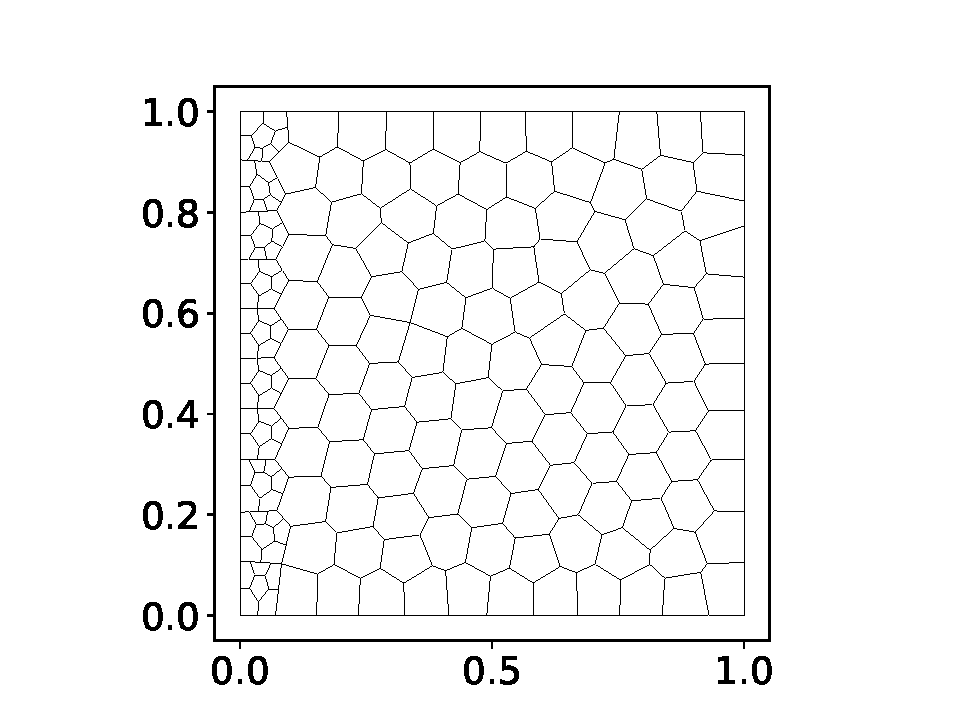
\includegraphics[trim=1cm 0.5cm 1cm 0.5cm, clip, width=0.3\textwidth]{meshes/adaptive/square_h_5.pdf}
	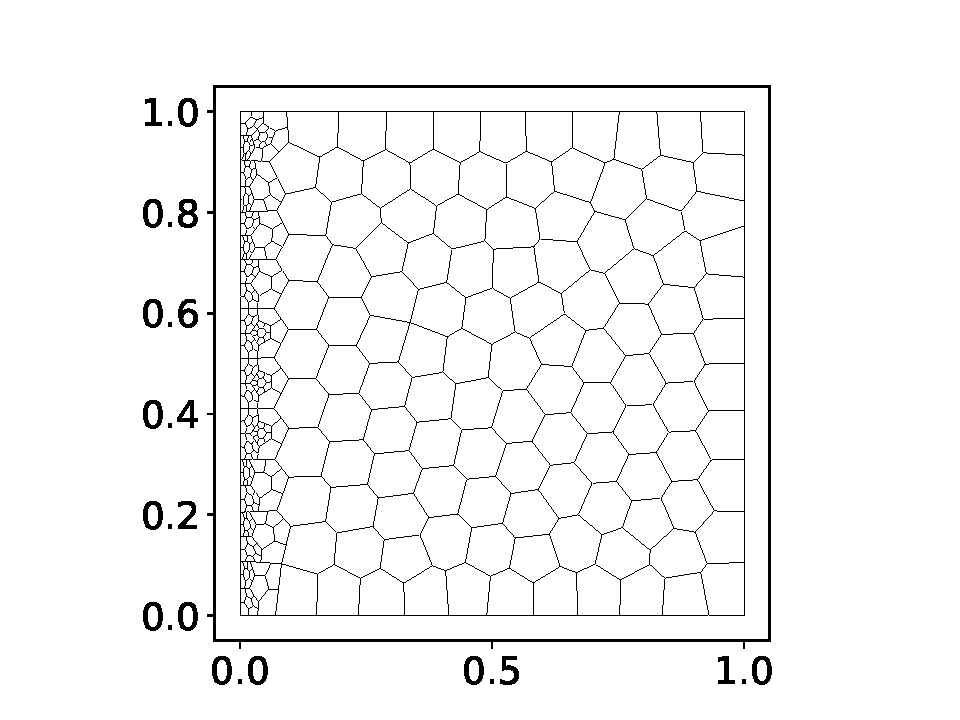
\includegraphics[trim=1cm 0.5cm 1cm 0.5cm, clip, width=0.3\textwidth]{meshes/adaptive/square_h_10.pdf}
	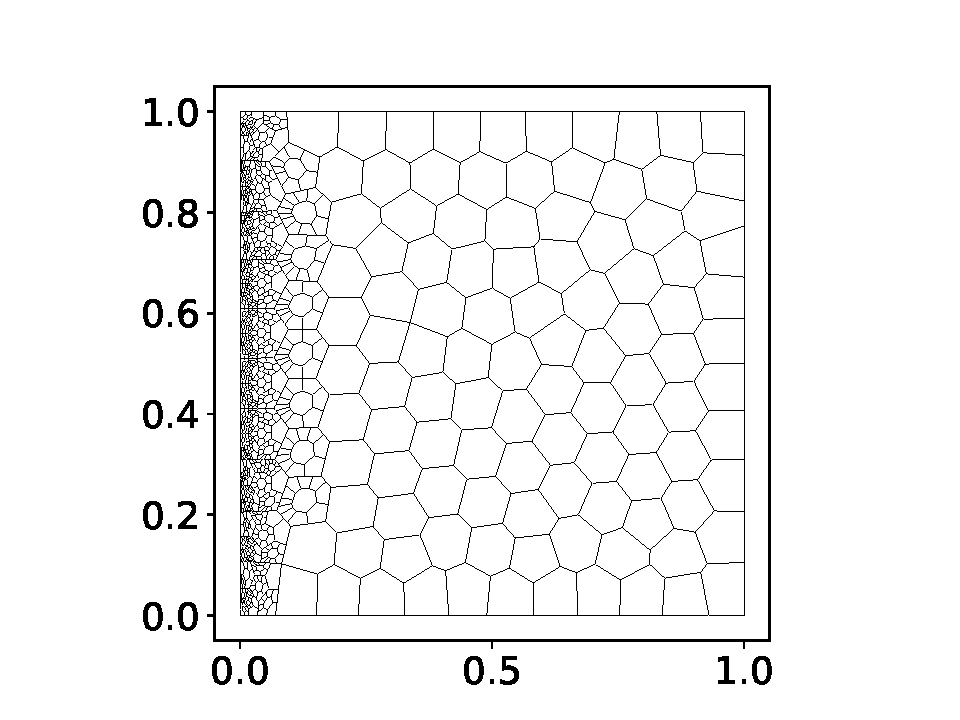
\includegraphics[trim=1cm 0.5cm 1cm 0.5cm, clip, width=0.3\textwidth]{meshes/adaptive/square_h_20.pdf}
	\caption{Square mesh after 5, 10, and 20 refinements, $N_0 = 125$.}
\end{figure}

\begin{figure}[!ht]
	\centering
	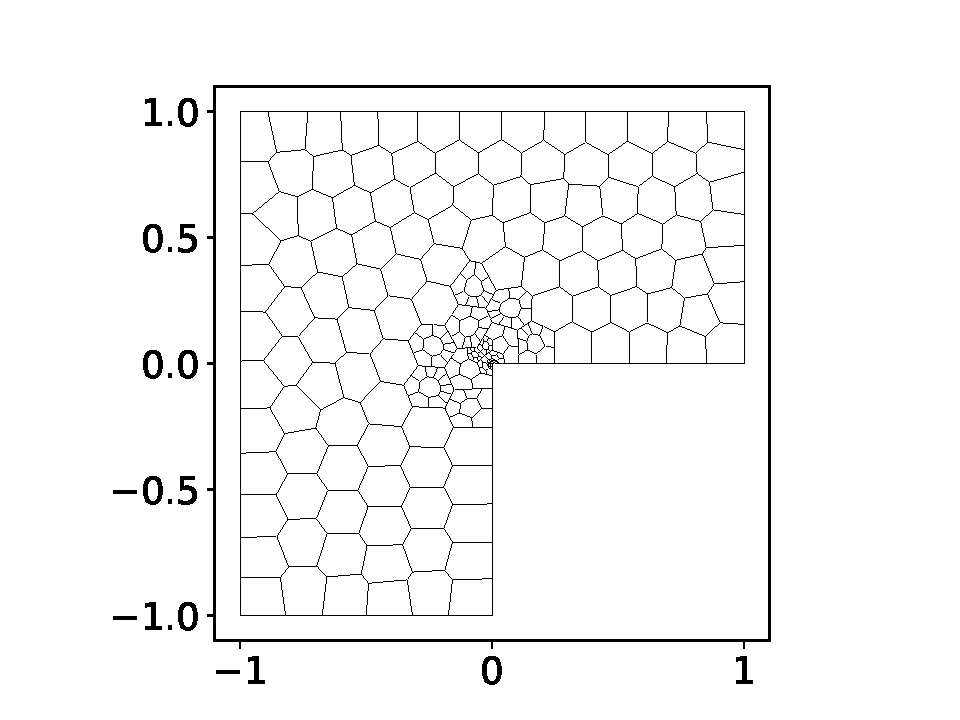
\includegraphics[trim=1cm 0.5cm 1cm 0.5cm, clip, width=0.3\textwidth]{meshes/adaptive/lshape_h_5.pdf}
	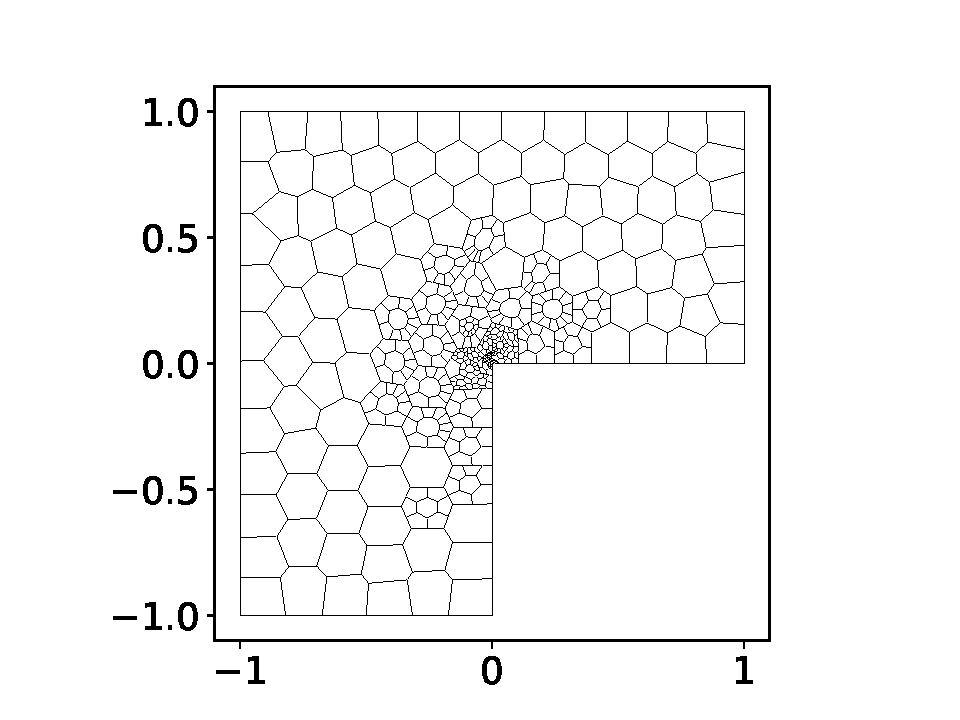
\includegraphics[trim=1cm 0.5cm 1cm 0.5cm, clip, width=0.3\textwidth]{meshes/adaptive/lshape_h_10.pdf}
	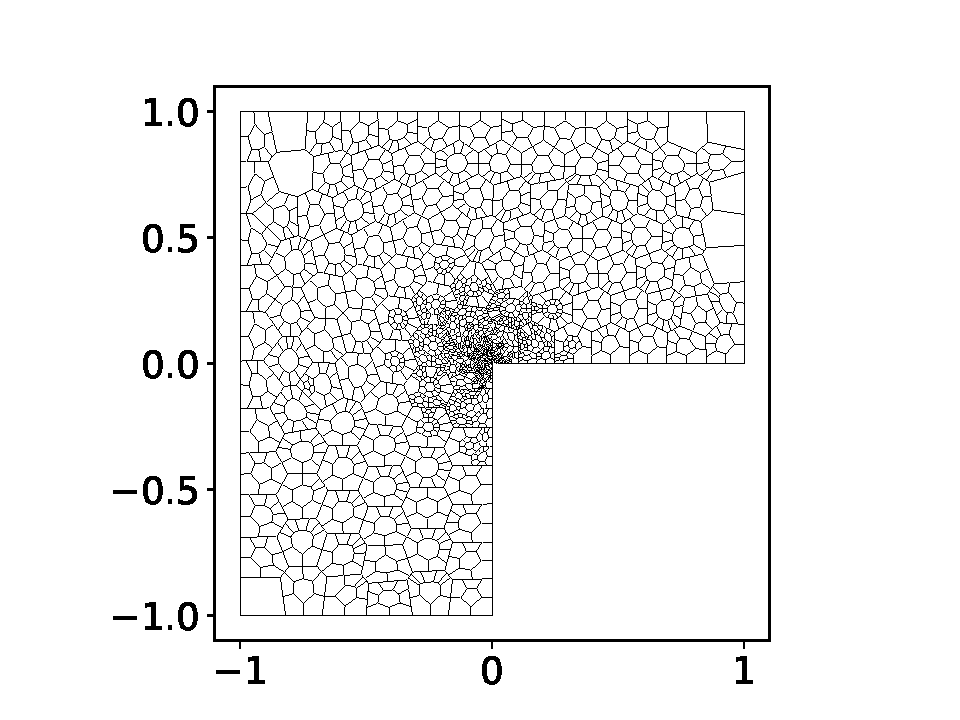
\includegraphics[trim=1cm 0.5cm 1cm 0.5cm, clip, width=0.3\textwidth]{meshes/adaptive/lshape_h_20.pdf}
	\caption{L-shaped mesh after 5, 10, and 20 refinements, $N_0 = 125$.}
\end{figure}

\newpage

Meshes refined based on local $\HO$ errors exhibit more concentrated refinement, demonstrating once again the superior approach provided by $\HO$ errors for these particular solutions.

\begin{figure}[!ht]
	\centering
	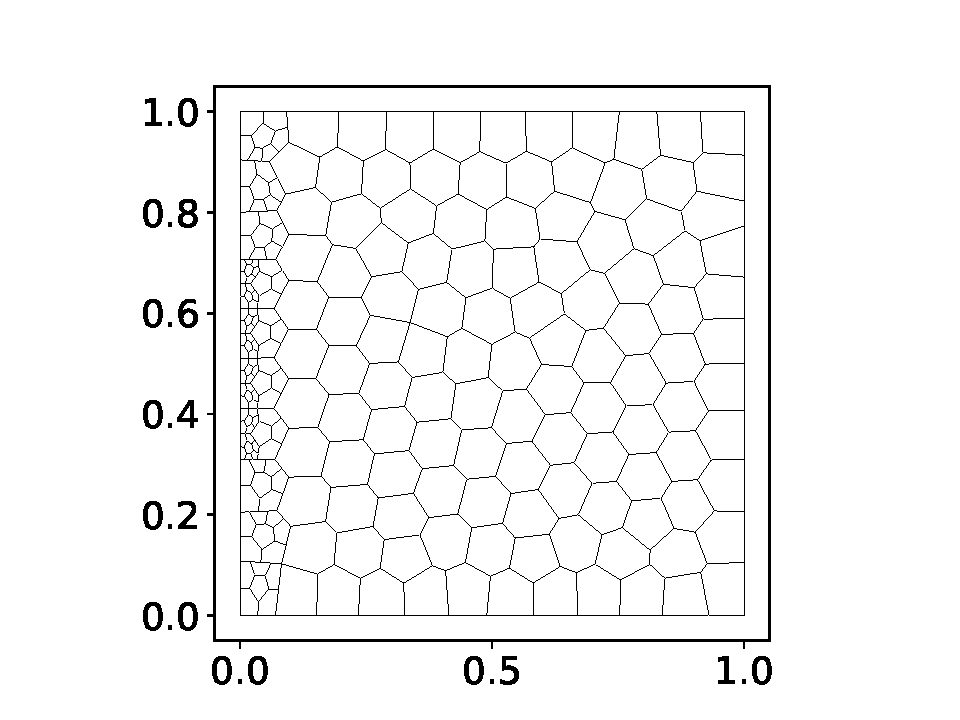
\includegraphics[trim=1cm 0.5cm 1cm 0.5cm, clip, width=0.3\textwidth]{meshes/adaptive/square_gh_5.pdf}
	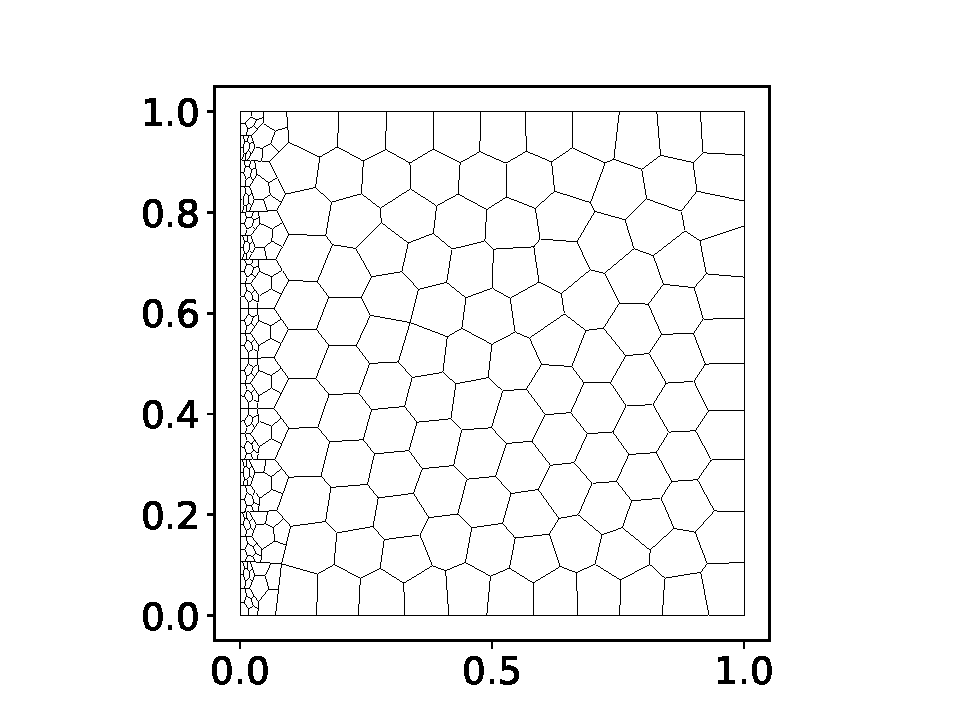
\includegraphics[trim=1cm 0.5cm 1cm 0.5cm, clip, width=0.3\textwidth]{meshes/adaptive/square_gh_10.pdf}
	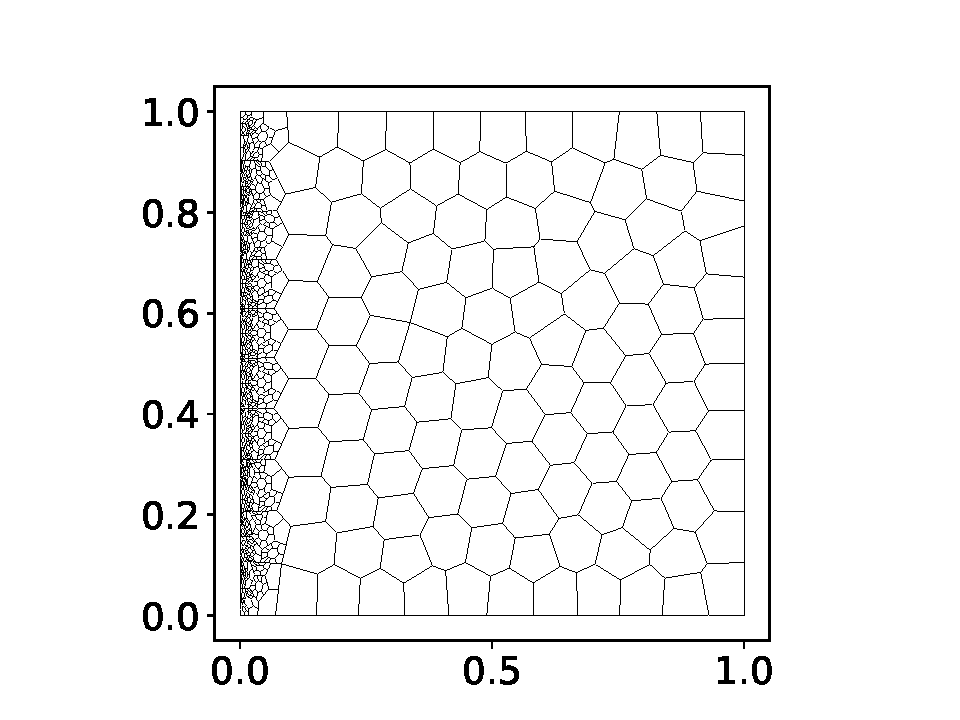
\includegraphics[trim=1cm 0.5cm 1cm 0.5cm, clip, width=0.3\textwidth]{meshes/adaptive/square_gh_20.pdf}
	\caption{Square mesh after 5, 10, and 20 refinements, $N_0 = 125$.}
\end{figure}

\begin{figure}[!ht]
	\centering
	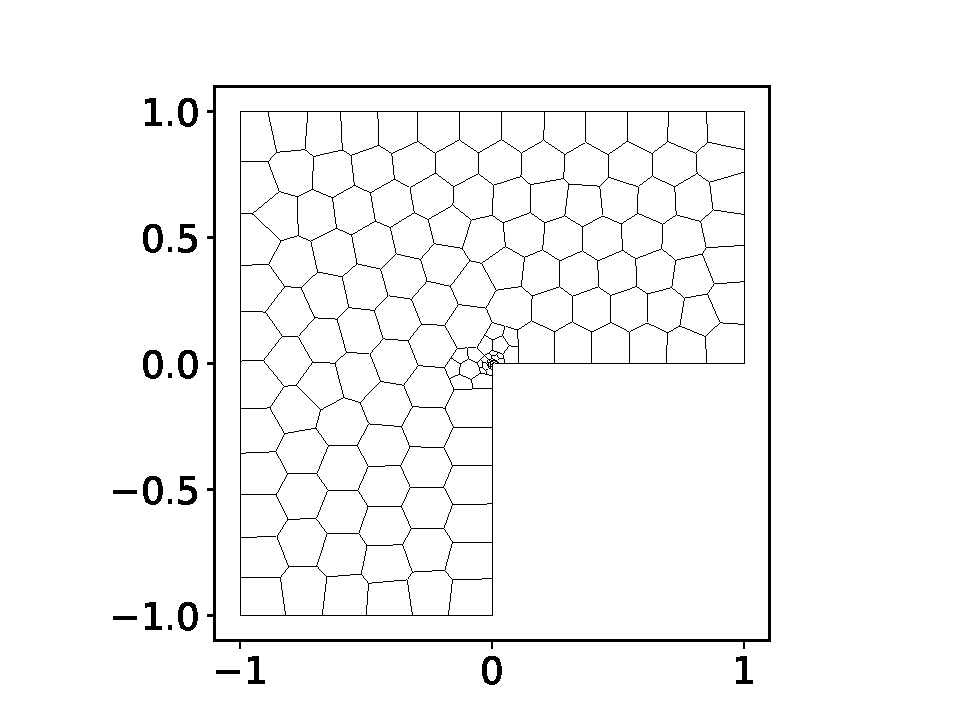
\includegraphics[trim=1cm 0.5cm 1cm 0.5cm, clip, width=0.3\textwidth]{meshes/adaptive/lshape_gh_5.pdf}
	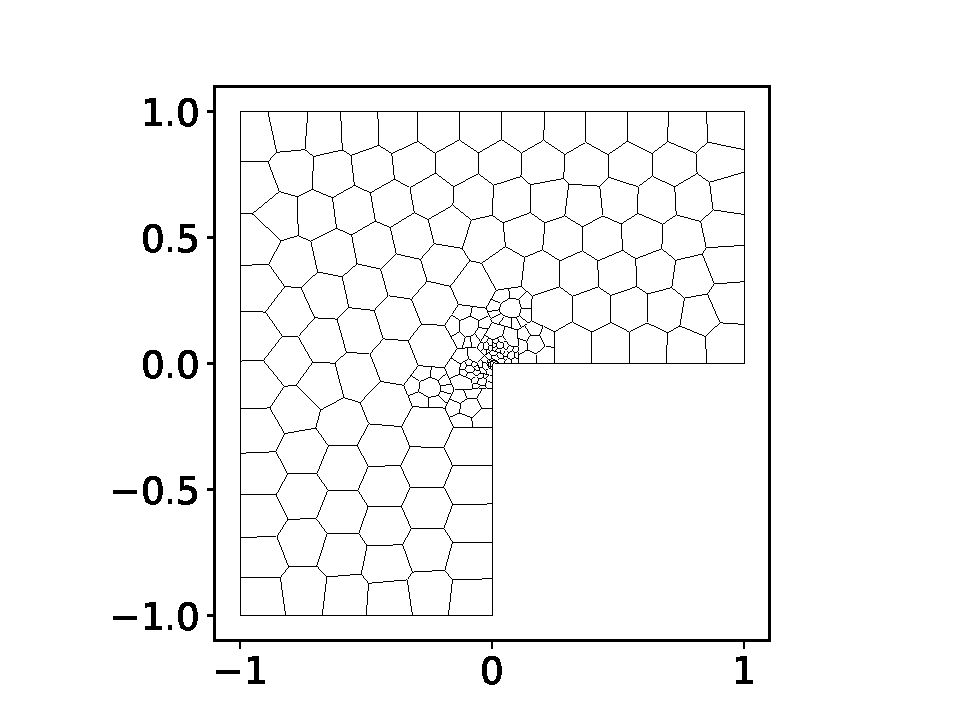
\includegraphics[trim=1cm 0.5cm 1cm 0.5cm, clip, width=0.3\textwidth]{meshes/adaptive/lshape_gh_10.pdf}
	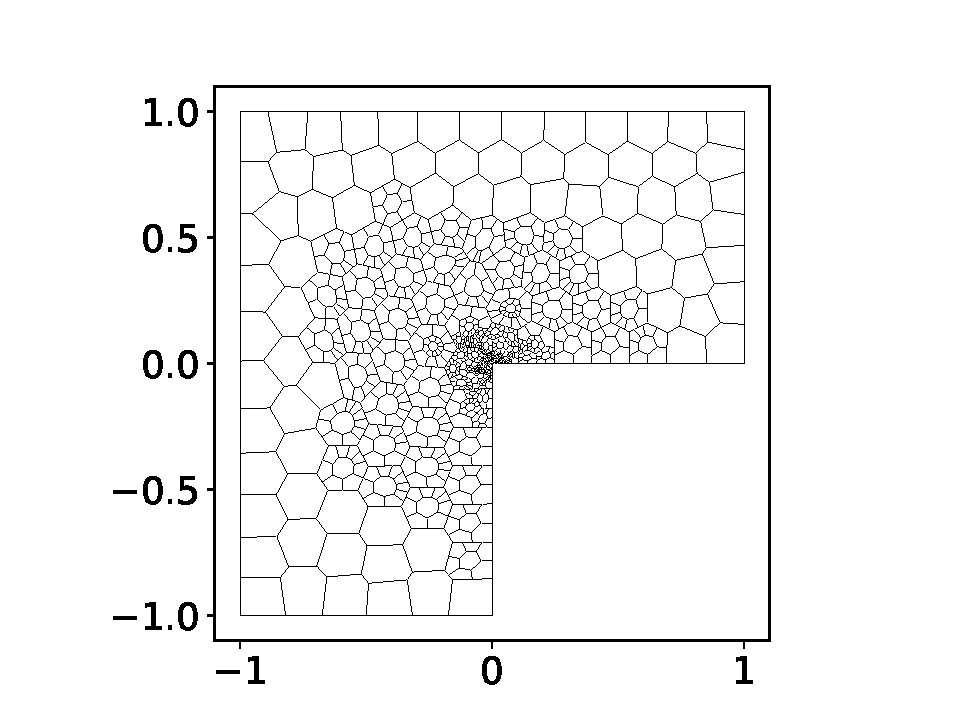
\includegraphics[trim=1cm 0.5cm 1cm 0.5cm, clip, width=0.3\textwidth]{meshes/adaptive/lshape_gh_20.pdf}
	\caption{L-shaped mesh after 5, 10, and 20 refinements, $N_0 = 125$.}
\end{figure}

\newpage
\subsection{A posteriori error estimates}

The second step in implementing \textit{h-adaptivity} is to define an \textit{a posteriori} error estimator, which enables the identification of elements that need refinement without requiring any information about the exact solution.

\cite{Cangiani2023} One possible approach considers the following upper bound on the error:

\begin{gather}
	\lVert u - u^k_h \rVert_{\LT(\Omega)} \leq C_{ub} \sum_{K \in \Tau_h} (R_K^2 + O_K^2),
\end{gather}

where:

\begin{gather}
	R_K^2 = R_{K, E}^2 + R_{K, N}^2 + R_{K, J}^2 + R_{K, T}^2
\end{gather}

is the local estimator and:

\begin{gather}
	O_K^2 = O_{K, E}^2 + O_{K, J}^2 + O_{K, T}^2
\end{gather}

is the local data oscillation. Each term is given by:

\begin{align}
	R_{K, E} &= \lVert h (\bar{f} + \Delta u^k_h) \rVert_{\LT(K)}, \\
	R_{K, N} &= \lVert h^{1/2} \llbracket \grad u^k_h \cdot \Vector{n} \rrbracket \rVert_{\LT(\partial K)}, \\
	R^2_{K, J} &= \lVert \gamma^{1/2} \llbracket u^k_h \rrbracket \rVert^2_{\LT(\partial K \cap \Gamma_{i})} + \lVert \gamma^{1/2} (u^k_h - \bar{g}) \rVert^2_{\LT(\partial K \cap \partial \Omega)}, \\
	R^2_{K, T} &= \lVert h^{1/2} \llbracket \grad u^k_h \cdot \Vector{e} \rrbracket \rVert^2_{\LT(\partial K \cap \Gamma_{i})} + \lVert \gamma^{1/2} \grad (u^k_h - \bar{g}) \cdot \Vector{e} \rVert^2_{\LT(\partial K \cap \partial \Omega)}, \\
	O_{K, E} &= \lVert h (f - \bar{f}) \rVert_{\LT(K)}, \\
	O_{K, J} &= \lVert \gamma^{1/2} (g - \bar{g}) \rVert_{\LT(\partial K \cap \partial \Omega)}, \\
	O_{K, T} &= \lVert h^{1/2} \grad (g - \bar{g}) \cdot \Vector{e} \rVert_{\LT(\partial K \cap \partial \Omega)}.
\end{align}

Here, $h$ represents the element size, $\gamma$ denotes the penalty coefficient for a given edge, and $\Vector{e}$ represents the unit vector along a given edge for tangent gradients.

\newpage
\subsubsection{Errors}

These error trends show that the \textit{a posteriori} error estimates (blue) behave similarly to the \textit{a priori} estimates (black). Additionally, in the case of the L-shaped domain, they exhibit improved behavior due to more concentrated refinement in the region of greatest interest. This is due to the significant local data oscillation caused by the singularity of $\grad u$ at the origin for this particular low-regularity solution.

\begin{figure}[!ht]
	\begin{subfigure}[b]{0.45\textwidth}
		% Errors v DOFs template for TikZ.

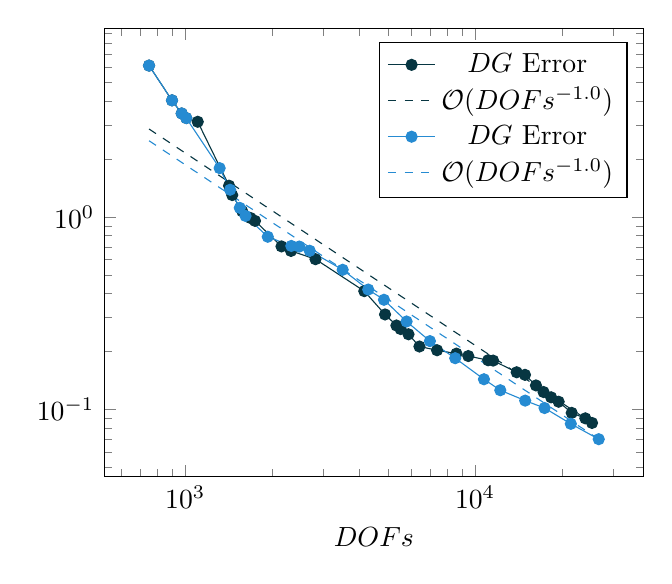
\begin{tikzpicture}
\begin{loglogaxis}[
    xlabel={$DOFs$},
    legend pos=north east,
]

\addplot[solarized-base02, mark=*] coordinates {(750,6.12566) (900,4.03955) (972,3.45362) (1008,3.26799) (1104,3.12636) (1416,1.45431) (1452,1.30003) (1572,1.0716) (1680,0.987916) (1740,0.954643) (2148,0.70325) (2316,0.666102) (2814,0.603387) (4146,0.411693) (4890,0.311397) (5352,0.272847) (5532,0.261592) (5892,0.245583) (6426,0.212127) (7392,0.202913) (8622,0.194848) (9474,0.189286) (11094,0.180045) (11538,0.179227) (13914,0.155865) (14862,0.151127) (16218,0.133144) (17226,0.123047) (18294,0.11549) (19422,0.109519) (21546,0.0958461) (24006,0.0897779) (25320,0.0849597)};
\addlegendentry{$DG$ Error}

\addplot[solarized-base02, dashed] coordinates {(750,2.868239472) (25320,0.0849597)};
\addlegendentry{$\mathcal{O}(DOFs^{-1.0})$}

\addplot[\accentcolor, mark=*] coordinates {(750,6.12566) (900,4.03955) (972,3.45362) (1008,3.26799) (1314,1.79461) (1428,1.38556) (1542,1.11532) (1614,1.01291) (1926,0.78948) (2322,0.707091) (2472,0.701825) (2688,0.667295) (3492,0.531519) (4278,0.419556) (4848,0.371234) (5802,0.286217) (6984,0.22631) (8538,0.184473) (10728,0.143353) (12216,0.125698) (14886,0.111004) (17364,0.101579) (21396,0.0840658) (26706,0.0699521)};
\addlegendentry{$DG$ Error}

\addplot[\accentcolor, dashed] coordinates {(750,2.4908543767999998) (26706,0.0699521)};
\addlegendentry{$\mathcal{O}(DOFs^{-1.0})$}

\end{loglogaxis}
\end{tikzpicture}
	\end{subfigure}
	\hfill
	\begin{subfigure}[b]{0.45\textwidth}
		% Errors v DOFs template for TikZ.

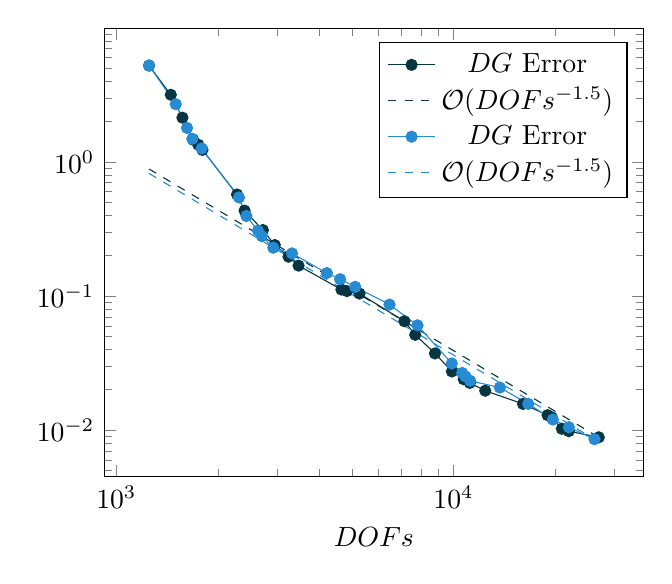
\begin{tikzpicture}
\begin{loglogaxis}[
    xlabel={$DOFs$},
    legend pos=north east,
]

\addplot[solarized-base02, mark=*] coordinates {(1250,5.22824) (1450,3.16847) (1570,2.13764) (1690,1.46207) (1750,1.34315) (1800,1.22937) (2280,0.571535) (2400,0.433165) (2720,0.310514) (2950,0.239953) (3240,0.196515) (3470,0.168581) (4650,0.111757) (4830,0.108861) (5260,0.104274) (7150,0.0648557) (7700,0.0513934) (8810,0.0373304) (9890,0.0273954) (10720,0.0239574) (11180,0.0225082) (12420,0.0196702) (16070,0.0156938) (19010,0.0129343) (19560,0.0124709) (20950,0.0102387) (21970,0.00982763) (26960,0.00884522)};
\addlegendentry{$DG$ Error}

\addplot[solarized-base02, dashed] coordinates {(1250,0.8859790477668384) (26960,0.00884522)};
\addlegendentry{$\mathcal{O}(DOFs^{-1.5})$}

\addplot[\accentcolor, mark=*] coordinates {(1250,5.22824) (1500,2.69514) (1620,1.7934) (1680,1.48702) (1790,1.25894) (2310,0.543447) (2430,0.395368) (2630,0.307434) (2700,0.279644) (2920,0.229209) (3320,0.207952) (4210,0.148303) (4610,0.133591) (5110,0.117099) (6460,0.0863494) (7820,0.0604748) (9880,0.0314321) (10610,0.0267064) (10850,0.0251548) (11200,0.0233236) (13720,0.0207803) (16660,0.0156883) (19710,0.0119851) (21980,0.0105234) (26180,0.00856227)};
\addlegendentry{$DG$ Error}

\addplot[\accentcolor, dashed] coordinates {(1250,0.8206885275389775) (26180,0.00856227)};
\addlegendentry{$\mathcal{O}(DOFs^{-1.5})$}

\end{loglogaxis}
\end{tikzpicture}
	\end{subfigure}
    \caption{$DG$ errors versus $DOFs$ comparison between adaptively refined meshes over a square domain. $k = 2$ (left) and $k = 3$ (right).}
\end{figure}

\begin{figure}[!ht]
	\begin{subfigure}[b]{0.45\textwidth}
		% Errors v DOFs template for TikZ.

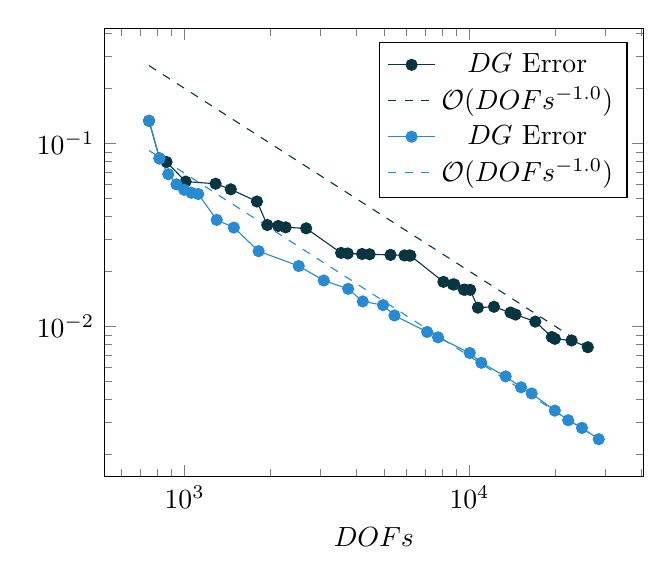
\begin{tikzpicture}
\begin{loglogaxis}[
    xlabel={$DOFs$},
    legend pos=north east,
]

\addplot[solarized-base02, mark=*] coordinates {(750,0.13327) (816,0.0830244) (864,0.0793426) (1008,0.0619878) (1284,0.0603523) (1452,0.0562495) (1794,0.0482533) (1950,0.0358904) (2130,0.0354704) (2262,0.0348557) (2670,0.0344147) (3540,0.0252647) (3738,0.0250711) (4194,0.0249254) (4458,0.0248335) (5280,0.0246302) (5910,0.0244758) (6132,0.0244387) (6198,0.0244288) (8094,0.0175423) (8742,0.0169922) (8838,0.0169865) (9546,0.015904) (9660,0.015896) (10050,0.015861) (10698,0.0126811) (12180,0.0128159) (13926,0.0119234) (14502,0.0116229) (17016,0.0106359) (19446,0.00875964) (19938,0.00856267) (22806,0.00838982) (26004,0.00770473)};
\addlegendentry{$DG$ Error}

\addplot[solarized-base02, dashed] coordinates {(750,0.26713839856000005) (26004,0.00770473)};
\addlegendentry{$\mathcal{O}(DOFs^{-1.0})$}

\addplot[\accentcolor, mark=*] coordinates {(750,0.13327) (816,0.0830244) (876,0.0680097) (936,0.0598727) (996,0.0559014) (1056,0.0538816) (1116,0.0530303) (1296,0.0382955) (1488,0.0347494) (1818,0.0258365) (2514,0.021412) (3078,0.0178477) (3750,0.0160642) (4218,0.0137184) (4968,0.0130898) (5448,0.0114913) (7098,0.0093373) (7752,0.00872489) (10020,0.007165) (10998,0.00633046) (13392,0.00533555) (15168,0.00465232) (16518,0.00430527) (19920,0.00346828) (22188,0.00307256) (24804,0.00278921) (28410,0.00242059)};
\addlegendentry{$DG$ Error}

\addplot[\accentcolor, dashed] coordinates {(750,0.0916919492) (28410,0.00242059)};
\addlegendentry{$\mathcal{O}(DOFs^{-1.0})$}

\end{loglogaxis}
\end{tikzpicture}
	\end{subfigure}
	\hfill
	\begin{subfigure}[b]{0.45\textwidth}
		% Errors v DOFs template for TikZ.

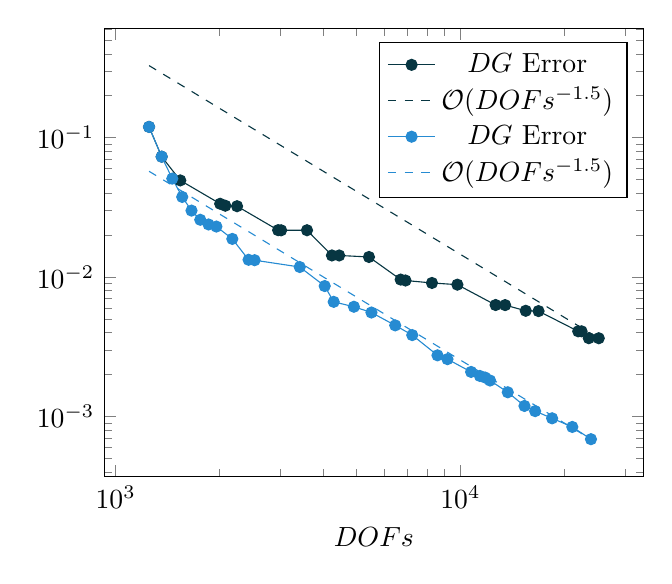
\begin{tikzpicture}
\begin{loglogaxis}[
    xlabel={$DOFs$},
    legend pos=north east,
]

\addplot[solarized-base02, mark=*] coordinates {(1250,0.119546) (1360,0.0730976) (1540,0.0493759) (2010,0.0335623) (2080,0.0325106) (2250,0.0322421) (2960,0.0217044) (3020,0.0216543) (3590,0.0216774) (4240,0.0142896) (4450,0.0142875) (5430,0.0139307) (6710,0.009591) (6930,0.0094454) (8270,0.00907011) (9800,0.00881814) (12650,0.00629972) (13480,0.00629107) (15470,0.00572756) (16850,0.00569782) (21960,0.00407968) (22460,0.00407912) (23570,0.00364227) (25190,0.00363907)};
\addlegendentry{$DG$ Error}

\addplot[solarized-base02, dashed] coordinates {(1250,0.3292059237674489) (25190,0.00363907)};
\addlegendentry{$\mathcal{O}(DOFs^{-1.5})$}

\addplot[\accentcolor, mark=*] coordinates {(1250,0.119546) (1360,0.0730976) (1460,0.0508708) (1560,0.0375773) (1660,0.0299764) (1760,0.0257653) (1860,0.0238484) (1960,0.0230301) (2180,0.0187842) (2430,0.0133021) (2530,0.0132102) (3420,0.0118042) (4040,0.00861783) (4290,0.00663868) (4910,0.00612195) (5520,0.00556495) (6470,0.00450029) (7250,0.00383231) (8580,0.00274332) (9170,0.00257528) (10740,0.00208511) (11390,0.0019513) (11790,0.00190163) (12190,0.0018094) (13720,0.00149002) (15340,0.00118862) (16470,0.00109125) (18450,0.000969034) (21110,0.000840165) (23910,0.000686294)};
\addlegendentry{$DG$ Error}

\addplot[\accentcolor, dashed] coordinates {(1250,0.05741356925713827) (23910,0.000686294)};
\addlegendentry{$\mathcal{O}(DOFs^{-1.5})$}

\end{loglogaxis}
\end{tikzpicture} % Incomplete.
	\end{subfigure}
    \caption{$DG$ errors versus $DOFs$ comparison between adaptively refined meshes over an L-shaped domain. $k = 2$ (left) and $k = 3$ (right).}
\end{figure}

\newpage

A better comparison can be made with respect to the $\HO$ refinement, where the \textit{a posteriori} estimates exhibit similar behavior.

\begin{figure}[!ht]
	\begin{subfigure}[b]{0.45\textwidth}
		% Errors v DOFs template for TikZ.

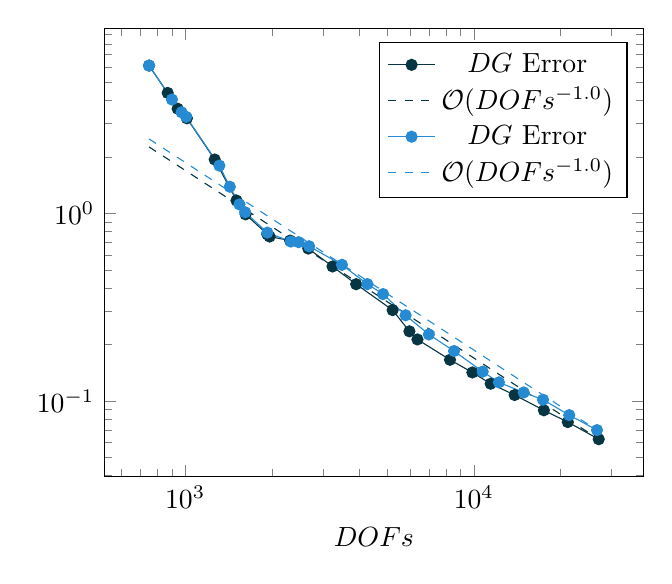
\begin{tikzpicture}
\begin{loglogaxis}[
    xlabel={$DOFs$},
    legend pos=north east,
]

\addplot[solarized-base02, mark=*] coordinates {(750,6.12566) (870,4.38193) (942,3.60957) (1014,3.20899) (1266,1.93506) (1506,1.16987) (1620,0.987314) (1926,0.773812) (1962,0.752143) (2310,0.715501) (2670,0.648814) (3240,0.520831) (3912,0.419024) (5232,0.304942) (5982,0.234997) (6378,0.212735) (8268,0.165754) (9882,0.141861) (11436,0.123541) (13848,0.107573) (17484,0.0891911) (21156,0.0771805) (27078,0.0625627)};
\addlegendentry{$DG$ Error}

\addplot[solarized-base02, dashed] coordinates {(750,2.2587637207999998) (27078,0.0625627)};
\addlegendentry{$\mathcal{O}(DOFs^{-1.0})$}

\addplot[\accentcolor, mark=*] coordinates {(750,6.12566) (900,4.03955) (972,3.45362) (1008,3.26799) (1314,1.79461) (1428,1.38556) (1542,1.11532) (1614,1.01291) (1926,0.78948) (2322,0.707091) (2472,0.701825) (2688,0.667295) (3492,0.531519) (4278,0.419556) (4848,0.371234) (5802,0.286217) (6984,0.22631) (8538,0.184473) (10728,0.143353) (12216,0.125698) (14886,0.111004) (17364,0.101579) (21396,0.0840658) (26706,0.0699521)};
\addlegendentry{$DG$ Error}

\addplot[\accentcolor, dashed] coordinates {(750,2.4908543767999998) (26706,0.0699521)};
\addlegendentry{$\mathcal{O}(DOFs^{-1.0})$}

\end{loglogaxis}
\end{tikzpicture}
	\end{subfigure}
	\hfill
	\begin{subfigure}[b]{0.45\textwidth}
		% Errors v DOFs template for TikZ.

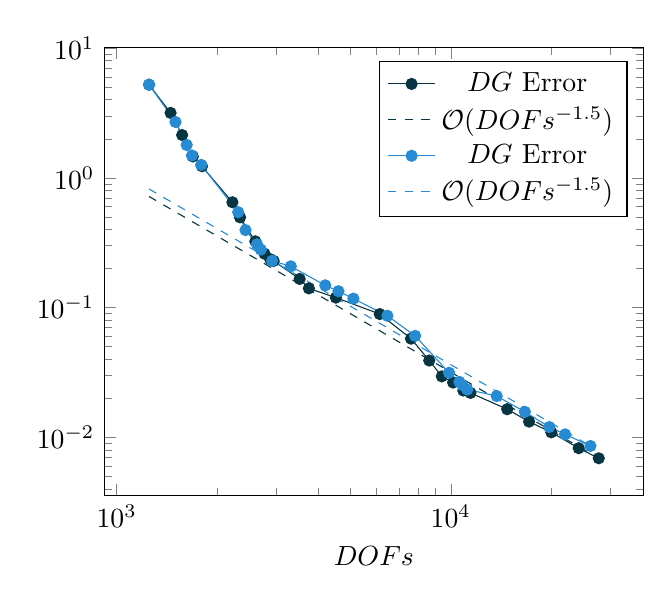
\begin{tikzpicture}
\begin{loglogaxis}[
    xlabel={$DOFs$},
    legend pos=north east,
]

\addplot[solarized-base02, mark=*] coordinates {(1250,5.22824) (1450,3.16847) (1570,2.13764) (1690,1.46207) (1800,1.22937) (2220,0.648223) (2340,0.495982) (2600,0.323852) (2770,0.260152) (2880,0.236183) (2950,0.22874) (3530,0.166199) (3760,0.140521) (4530,0.119187) (6130,0.089056) (7600,0.0575574) (8620,0.0390489) (9400,0.0294453) (10160,0.0263927) (10900,0.0229053) (11450,0.0219544) (14750,0.0164373) (17150,0.0131901) (19990,0.0109056) (24140,0.00823295) (27720,0.00688026)};
\addlegendentry{$DG$ Error}

\addplot[solarized-base02, dashed] coordinates {(1250,0.7185047930727512) (27720,0.00688026)};
\addlegendentry{$\mathcal{O}(DOFs^{-1.5})$}

\addplot[\accentcolor, mark=*] coordinates {(1250,5.22824) (1500,2.69514) (1620,1.7934) (1680,1.48702) (1790,1.25894) (2310,0.543447) (2430,0.395368) (2630,0.307434) (2700,0.279644) (2920,0.229209) (3320,0.207952) (4210,0.148303) (4610,0.133591) (5110,0.117099) (6460,0.0863494) (7820,0.0604748) (9880,0.0314321) (10610,0.0267064) (10850,0.0251548) (11200,0.0233236) (13720,0.0207803) (16660,0.0156883) (19710,0.0119851) (21980,0.0105234) (26180,0.00856227)};
\addlegendentry{$DG$ Error}

\addplot[\accentcolor, dashed] coordinates {(1250,0.8206885275389775) (26180,0.00856227)};
\addlegendentry{$\mathcal{O}(DOFs^{-1.5})$}

\end{loglogaxis}
\end{tikzpicture}
	\end{subfigure}
    \caption{$DG$ errors versus $DOFs$ comparison between adaptively refined meshes over a square domain. $k = 2$ (left) and $k = 3$ (right).}
\end{figure}

\begin{figure}[!ht]
	\begin{subfigure}[b]{0.45\textwidth}
		% Errors v DOFs template for TikZ.

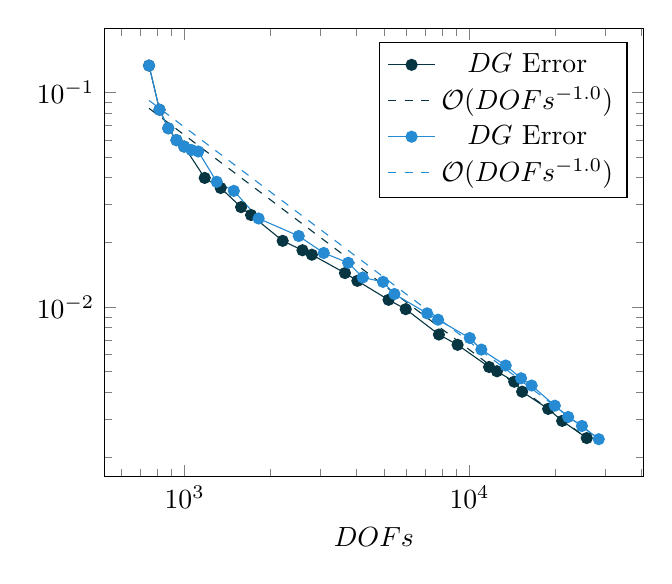
\begin{tikzpicture}
\begin{loglogaxis}[
    xlabel={$DOFs$},
    legend pos=north east,
]

\addplot[solarized-base02, mark=*] coordinates {(750,0.13327) (816,0.0830244) (876,0.0680097) (936,0.0598727) (996,0.0559014) (1176,0.039932) (1338,0.0358411) (1578,0.0291867) (1710,0.0268234) (2208,0.0203268) (2592,0.0183746) (2796,0.0175187) (3654,0.0143896) (4038,0.0132366) (5196,0.0107976) (5970,0.00976556) (7806,0.00743953) (9078,0.00666211) (11712,0.00525048) (12480,0.00501671) (14346,0.00448473) (15294,0.00402922) (18876,0.00335053) (21138,0.00294547) (25782,0.00244963)};
\addlegendentry{$DG$ Error}

\addplot[solarized-base02, dashed] coordinates {(750,0.08420848087999999) (25782,0.00244963)};
\addlegendentry{$\mathcal{O}(DOFs^{-1.0})$}

\addplot[\accentcolor, mark=*] coordinates {(750,0.13327) (816,0.0830244) (876,0.0680097) (936,0.0598727) (996,0.0559014) (1056,0.0538816) (1116,0.0530303) (1296,0.0382955) (1488,0.0347494) (1818,0.0258365) (2514,0.021412) (3078,0.0178477) (3750,0.0160642) (4218,0.0137184) (4968,0.0130898) (5448,0.0114913) (7098,0.0093373) (7752,0.00872489) (10020,0.007165) (10998,0.00633046) (13392,0.00533555) (15168,0.00465232) (16518,0.00430527) (19920,0.00346828) (22188,0.00307256) (24804,0.00278921) (28410,0.00242059)};
\addlegendentry{$DG$ Error}

\addplot[\accentcolor, dashed] coordinates {(750,0.0916919492) (28410,0.00242059)};
\addlegendentry{$\mathcal{O}(DOFs^{-1.0})$}

\end{loglogaxis}
\end{tikzpicture}
	\end{subfigure}
	\hfill
	\begin{subfigure}[b]{0.45\textwidth}
		% Errors v DOFs template for TikZ.

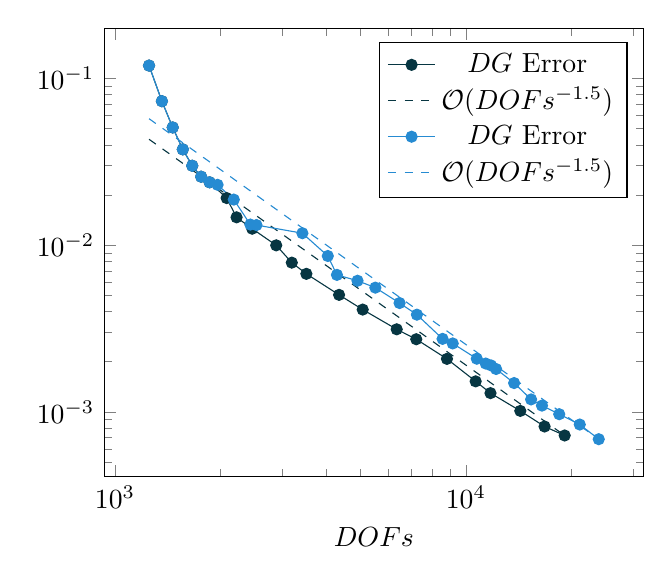
\begin{tikzpicture}
\begin{loglogaxis}[
    xlabel={$DOFs$},
    legend pos=north east,
]

\addplot[solarized-base02, mark=*] coordinates {(1250,0.119546) (1360,0.0730976) (1460,0.0508708) (1560,0.0375773) (1660,0.0299764) (1760,0.0257653) (1860,0.0238484) (2080,0.0191889) (2220,0.0147015) (2460,0.0125616) (2880,0.00998454) (3190,0.00786125) (3510,0.00673439) (4350,0.0050375) (5080,0.00411082) (6350,0.00313077) (7220,0.00272903) (8830,0.00208062) (10660,0.0015255) (11750,0.00129659) (14290,0.00101426) (16760,0.000817683) (19120,0.00072222)};
\addlegendentry{$DG$ Error}

\addplot[solarized-base02, dashed] coordinates {(1250,0.04320523018854778) (19120,0.00072222)};
\addlegendentry{$\mathcal{O}(DOFs^{-1.5})$}

\addplot[\accentcolor, mark=*] coordinates {(1250,0.119546) (1360,0.0730976) (1460,0.0508708) (1560,0.0375773) (1660,0.0299764) (1760,0.0257653) (1860,0.0238484) (1960,0.0230301) (2180,0.0187842) (2430,0.0133021) (2530,0.0132102) (3420,0.0118042) (4040,0.00861783) (4290,0.00663868) (4910,0.00612195) (5520,0.00556495) (6470,0.00450029) (7250,0.00383231) (8580,0.00274332) (9170,0.00257528) (10740,0.00208511) (11390,0.0019513) (11790,0.00190163) (12190,0.0018094) (13720,0.00149002) (15340,0.00118862) (16470,0.00109125) (18450,0.000969034) (21110,0.000840165) (23910,0.000686294)};
\addlegendentry{$DG$ Error}

\addplot[\accentcolor, dashed] coordinates {(1250,0.05741356925713827) (23910,0.000686294)};
\addlegendentry{$\mathcal{O}(DOFs^{-1.5})$}

\end{loglogaxis}
\end{tikzpicture} % Incomplete.
	\end{subfigure}
    \caption{$DG$ errors versus $DOFs$ comparison between adaptively refined meshes over an L-shaped domain. $k = 2$ (left) and $k = 3$ (right).}
\end{figure}

\newpage
\subsubsection{Meshes}

Meshes refined using \textit{a posteriori} error estimates exhibit more concentrated refinement compared to those refined using \textit{a priori} error estimates.

\begin{figure}[!ht]
	\centering
	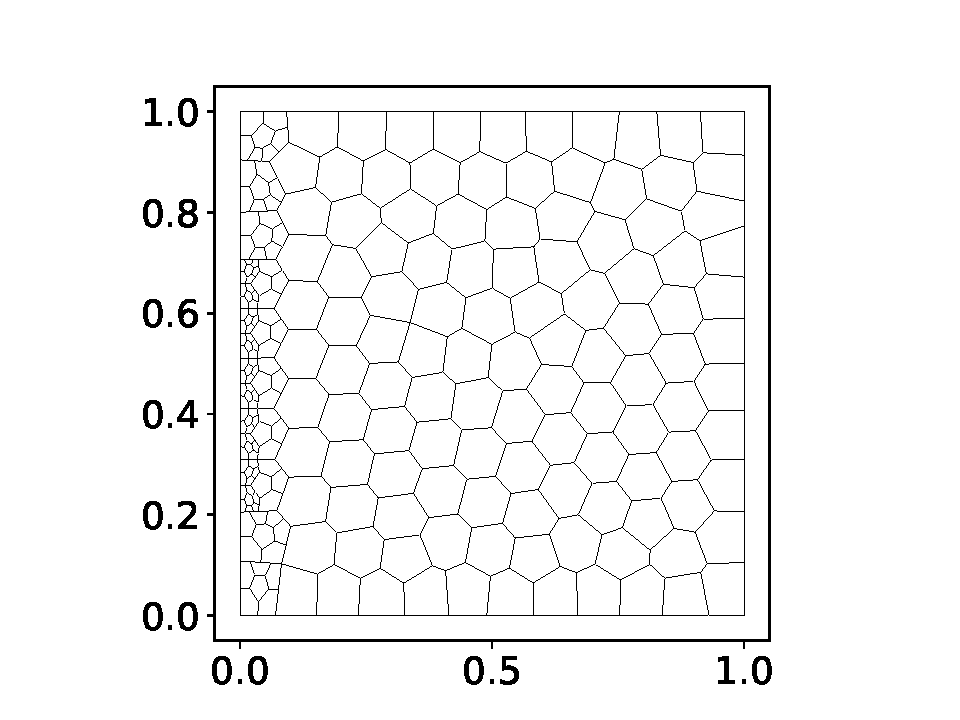
\includegraphics[trim=1cm 0.5cm 1cm 0.5cm, clip, width=0.3\textwidth]{meshes/adaptive/square_eh_5.pdf}
	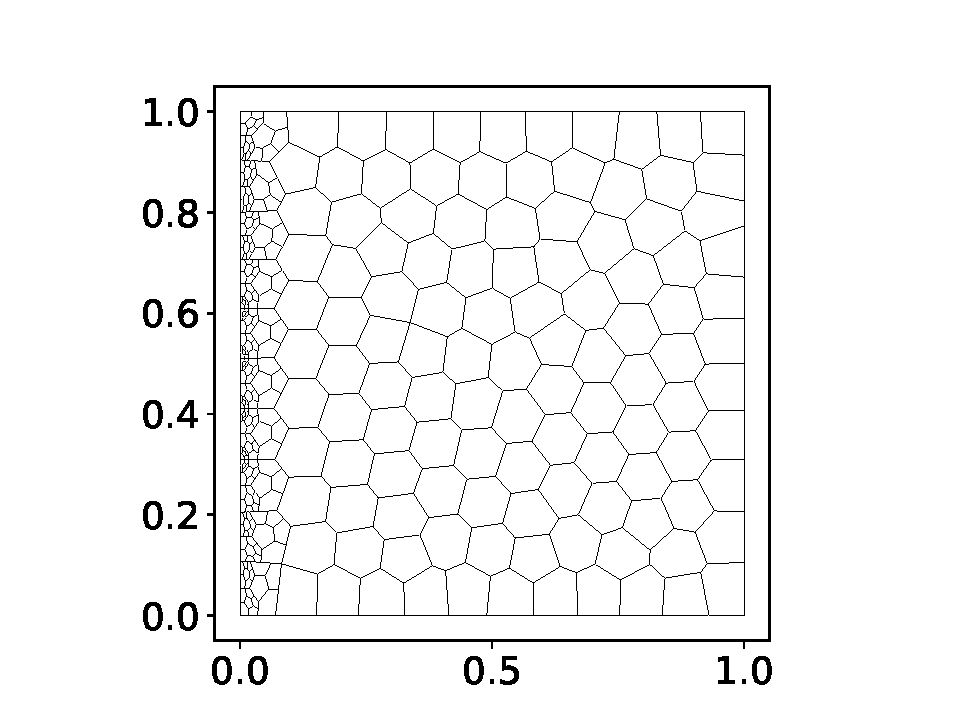
\includegraphics[trim=1cm 0.5cm 1cm 0.5cm, clip, width=0.3\textwidth]{meshes/adaptive/square_eh_10.pdf}
	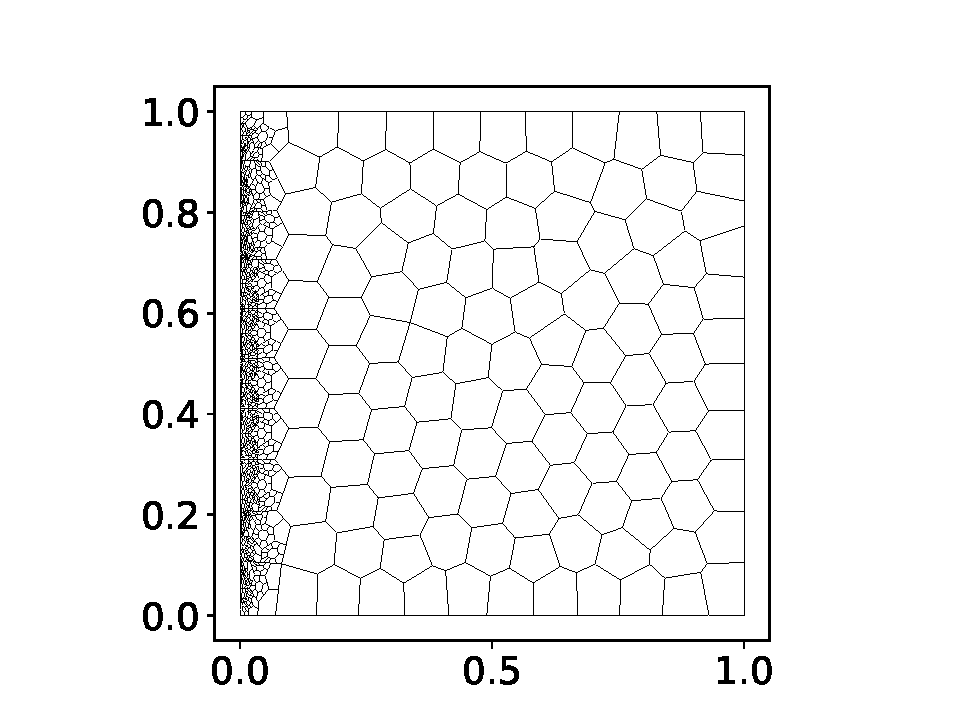
\includegraphics[trim=1cm 0.5cm 1cm 0.5cm, clip, width=0.3\textwidth]{meshes/adaptive/square_eh_20.pdf}
	\caption{Square mesh after 5, 10, and 20 refinements, $N_0 = 125$.}
\end{figure}

\begin{figure}[!ht]
	\centering
	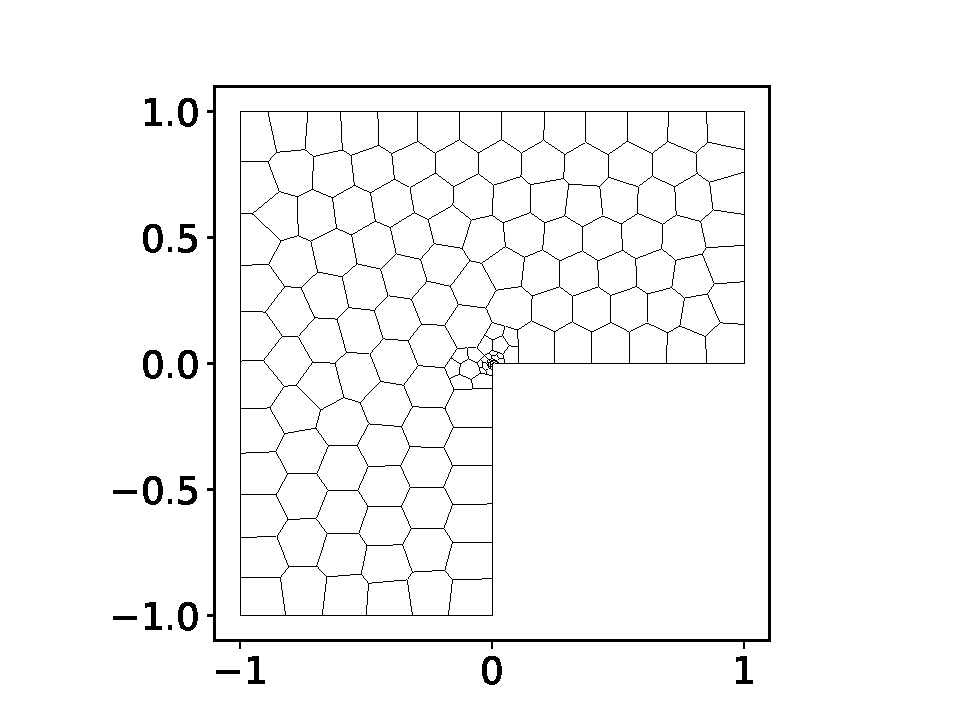
\includegraphics[trim=1cm 0.5cm 1cm 0.5cm, clip, width=0.3\textwidth]{meshes/adaptive/lshape_eh_5.pdf}
	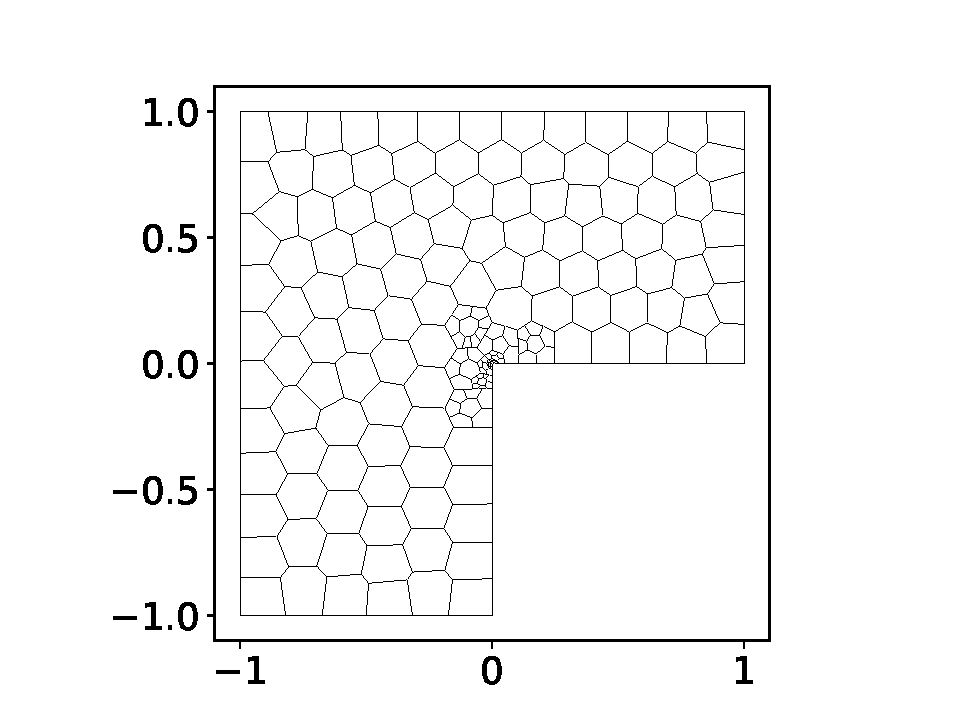
\includegraphics[trim=1cm 0.5cm 1cm 0.5cm, clip, width=0.3\textwidth]{meshes/adaptive/lshape_eh_10.pdf}
	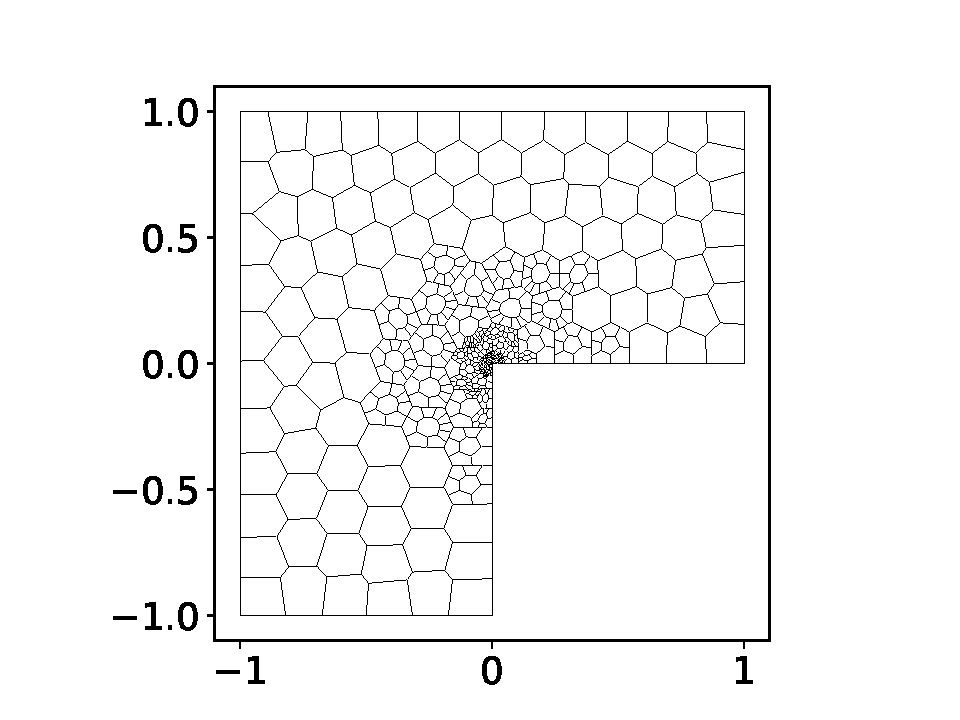
\includegraphics[trim=1cm 0.5cm 1cm 0.5cm, clip, width=0.3\textwidth]{meshes/adaptive/lshape_eh_20.pdf}
	\caption{L-shaped mesh after 5, 10, and 20 refinements, $N_0 = 125$.}
\end{figure}

\newpage
\subsection{A code snippet}

Here's a snippet to illustrate the \textit{h-adaptive} mesh refinement from the user's perspective:

\lstinputlisting[style=cpp, firstline=11]{../snippets/h_refine.cpp}

	\newpage
    \section{Implementing \textit{hp-Adaptivity}}
	\subsection{Estimating the decay rate of the Legendre coefficients}

Having tested the \textit{h-adaptive} refinement capabilities for this $DG$ implementation, the next and final step is to implement \textit{p-adaptive} refinement using a test of analyticity.

\cite{Eibner2007} Since the solution is represented by the coefficients of Legendre polynomials, analyticity can be assessed by evaluating their rate of decay.

Given \eqref{decomposition}, the following relation can be written for every element $K$:

\begin{gather}
    u^{k, ij}_{h, K} = c_{ij} \phi_{ij} \quad \Forall i, j : i + j = k.
\end{gather}

Assuming smoothness for $u^k_{h, K}$, the following holds:

\begin{gather}
    \Exists a_K, b_K \in \R : c_{ij} \approx a_K e^{-b_K (i + j)}.
\end{gather}

An estimate of $b_K$ through a linear fit of $\log(\lvert c_{ij} \rvert)$ is the key to choosing \textit{p-refinement} over \textit{h-refinement}. In fact, $u^k_{h, K}$ is said to be smooth if $b_K$ exceeds a certain threshold, fixed to $1.0$ in the following numerical tests.

The marking strategy is slightly modified so that the elements $K$ to be refined are chosen in the following way:

\begin{gather}
    \eta_K^2 > \sigma \bar{\eta}^2,
\end{gather}

where:

\begin{gather}
    \bar{\eta}^2 = \frac{1}{\lvert \Tau \rvert} \sum_{K \in \Tau} \eta_K^2.
\end{gather}

\cite{Eibner2007} The expected convergence rates over the L-shaped domain for a singularity-bearing solution and the square domain for a smooth, albeit low-regularity, solution are:

\begin{gather} 
    \lVert u - u^k_h \rVert_{DG, \, \text{Square}} \approx a \, e^{-b \, \text{DOFs}^{1/2}}, \label{square-hp} \\
    \lVert u - u^k_h \rVert_{DG, \, \text{L-shape}} \approx a \, e^{-b \, \text{DOFs}^{1/3}}. \label{lshape-hp}
\end{gather}

\newpage
\subsubsection{Errors}

Tests with an initial polynomial degree of $k_0 = 1$ exhibit exponential error trends, confirming both \eqref{square-hp} and \eqref{lshape-hp}.

\begin{figure}[!ht]
    \begin{subfigure}[b]{0.45\textwidth}
		% HP v DOFs template for TikZ.

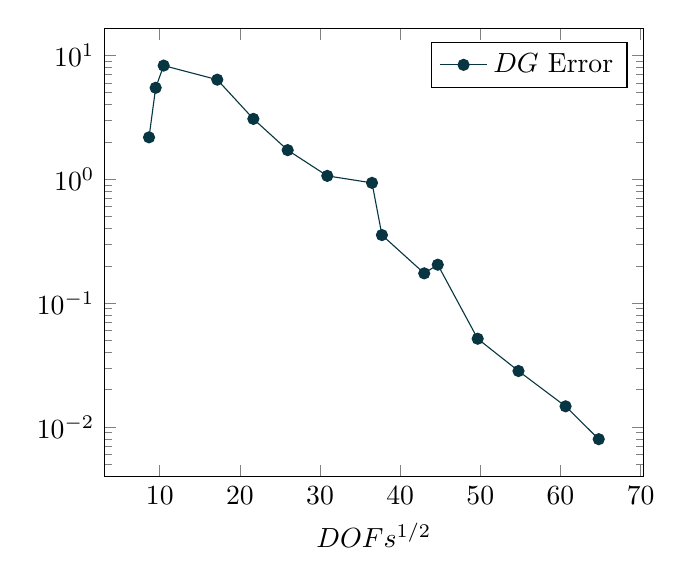
\begin{tikzpicture}
\begin{axis}[
    xlabel={$DOFs^{1/2}$}, % Edit if needed.
    legend pos=north east,
    ymode=log
]

\addplot[solarized-base02, mark=*] coordinates {(8.660254037844387,2.1812) (9.486832980505138,5.48286) (10.488088481701515,8.28706) (17.175564037317667,6.37634) (21.6794833886788,3.07509) (25.96150997149434,1.71936) (30.903074280724887,1.06513) (36.4828726939094,0.935197) (37.72267222772003,0.3543) (43.0,0.173769) (44.68780594300866,0.204124) (49.66890375275057,0.0514923) (54.76312628037227,0.0282501) (60.63827174318213,0.0146515) (64.77653896280658,0.0079507)};
\addlegendentry{$DG$ Error}

\end{axis}
\end{tikzpicture}
	\end{subfigure}
	\hfill
	\begin{subfigure}[b]{0.45\textwidth}
		% HP v DOFs template for TikZ.

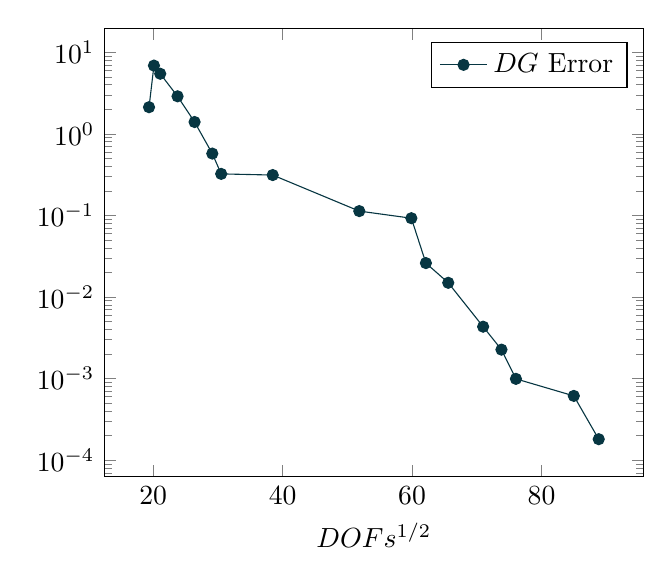
\begin{tikzpicture}
\begin{axis}[
    xlabel={$DOFs^{1/2}$}, % Edit if needed.
    legend pos=north east,
    ymode=log
]

\addplot[solarized-base02, mark=*] coordinates {(19.364916731037084,2.12045) (20.12461179749811,6.86265) (21.095023109728988,5.45188) (23.769728648009426,2.88383) (26.40075756488817,1.39635) (29.13760456866693,0.57264) (30.512292604784715,0.322807) (38.47076812334269,0.312358) (51.84592558726288,0.112932) (59.89156868875618,0.0923704) (62.13694553162394,0.0260415) (65.58963332722634,0.0149262) (70.97887009526144,0.00432584) (73.81056834898374,0.00226267) (76.04603868710059,0.000991637) (84.98823447983844,0.000613095) (88.83692925805124,0.000180696)};
\addlegendentry{$DG$ Error}

\end{axis}
\end{tikzpicture}
	\end{subfigure}
    \caption{$DG$ error versus $DOFs^{1/2}$ on a sequence of \textit{hp-adaptively} refined meshes over a square domain. $k_0 = 1$, $N_0 = 25$ (left) and $N_0 = 125$ (right).}
\end{figure}

\begin{figure}[!ht]
    \begin{subfigure}[b]{0.45\textwidth}
		% HP v DOFs template for TikZ.

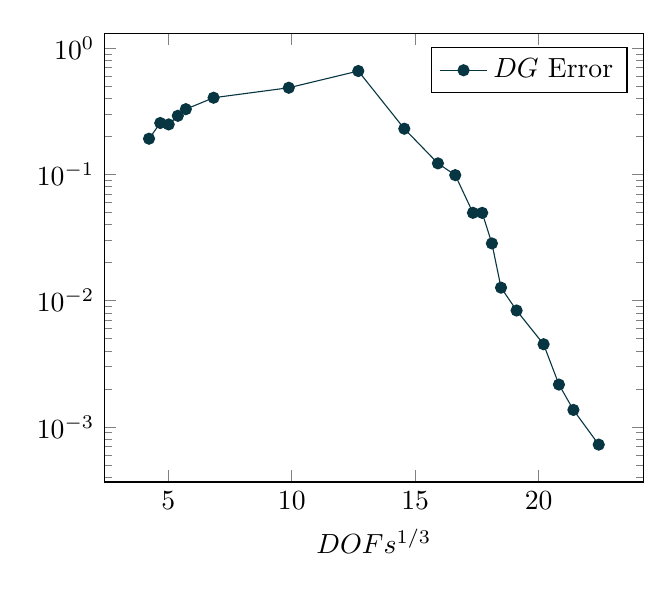
\begin{tikzpicture}
\begin{axis}[
    xlabel={$DOFs^{1/3}$}, % Edit if needed.
    legend pos=north east,
    ymode=log
]

\addplot[solarized-base02, mark=*] coordinates {(4.217163326508746,0.191755) (4.672328728355259,0.255398) (5.0132979349645845,0.248801) (5.383212612087283,0.291174) (5.708267473384861,0.328607) (6.832771452246442,0.404871) (9.878530490026034,0.485699) (12.69507321245234,0.659013) (14.55901434377428,0.230073) (15.921490395218942,0.122269) (16.623800957486996,0.098664) (17.340316055801914,0.0495985) (17.714635665253457,0.0495794) (18.10839938601742,0.0283923) (18.477938151928672,0.0126687) (19.10925056502305,0.00835058) (20.20211721754757,0.00451385) (20.823924640400417,0.00216312) (21.4106622851008,0.00136207) (22.436197851201577,0.00072339)};
\addlegendentry{$DG$ Error}

\end{axis}
\end{tikzpicture}
	\end{subfigure}
	\hfill
	\begin{subfigure}[b]{0.45\textwidth}
		% HP v DOFs template for TikZ.

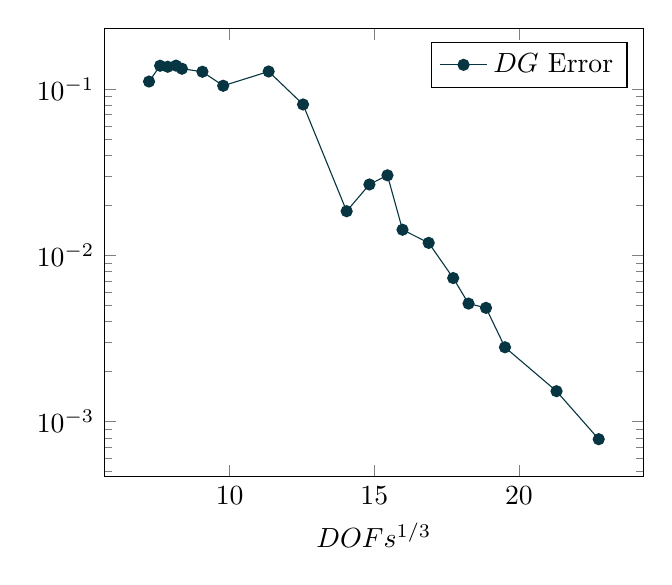
\begin{tikzpicture}
\begin{axis}[
    xlabel={$DOFs^{1/3}$}, % Edit if needed.
    legend pos=north east,
    ymode=log
]

\addplot[solarized-base02, mark=*] coordinates {(7.211247851537041,0.110732) (7.594363318174861,0.137827) (7.856828007847996,0.135903) (8.14325284978472,0.138095) (8.349125609133615,0.132241) (9.057248245324264,0.126807) (9.77497432636947,0.104464) (11.347061411356195,0.127274) (12.535896814815494,0.080649) (14.044078760203224,0.0184031) (14.830688695146508,0.0266482) (15.454252904182171,0.0302544) (15.975222064844958,0.0142437) (16.880359523050902,0.0118758) (17.72737313911207,0.00729791) (18.257612386946448,0.00512641) (18.86141077038746,0.00483127) (19.51762596542329,0.00280033) (21.299561365474005,0.00152487) (22.75930465103004,0.000784873)};
\addlegendentry{$DG$ Error}

\end{axis}
\end{tikzpicture}
	\end{subfigure}
    \caption{$DG$ error versus $DOFs^{1/3}$ on a sequence of \textit{hp-adaptively} refined meshes over an L-shaped domain. $k_0 = 1$, $N_0 = 25$ (left) and $N_0 = 125$ (right).}
\end{figure}

\newpage

Tests with an initial polynomial degree of $k_0 = 3$ exhibit an exponential error trend earlier than those with $k_0 = 1$, which is significant. However, this trend later deviates, most likely due to the worse ill-conditioning of $\MA$.

\begin{figure}[!ht]
    \begin{subfigure}[b]{0.45\textwidth}
		% HP v DOFs template for TikZ.

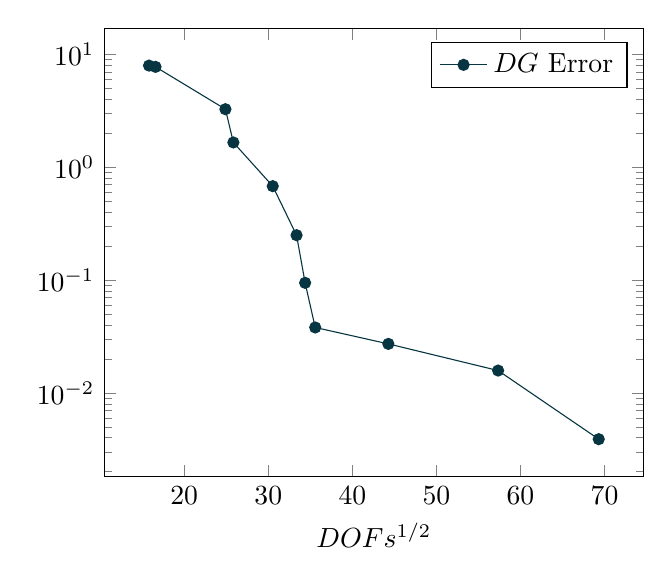
\begin{tikzpicture}
\begin{axis}[
    xlabel={$DOFs^{1/2}$}, % Edit if needed.
    legend pos=north east,
    ymode=log
]

\addplot[solarized-base02, mark=*] coordinates {(15.811388300841896,7.96311) (16.583123951777,7.75835) (24.899799195977465,3.26933) (25.84569596664017,1.6579) (30.528675044947494,0.679623) (33.36165463522455,0.249793) (34.38022687534217,0.0944762) (35.58089374931439,0.0380026) (44.28317965096906,0.0271763) (57.3410847473258,0.0157725) (69.31089380465383,0.00388741)};
\addlegendentry{$DG$ Error}

\end{axis}
\end{tikzpicture}
	\end{subfigure}
	\hfill
	\begin{subfigure}[b]{0.45\textwidth}
		% HP v DOFs template for TikZ.

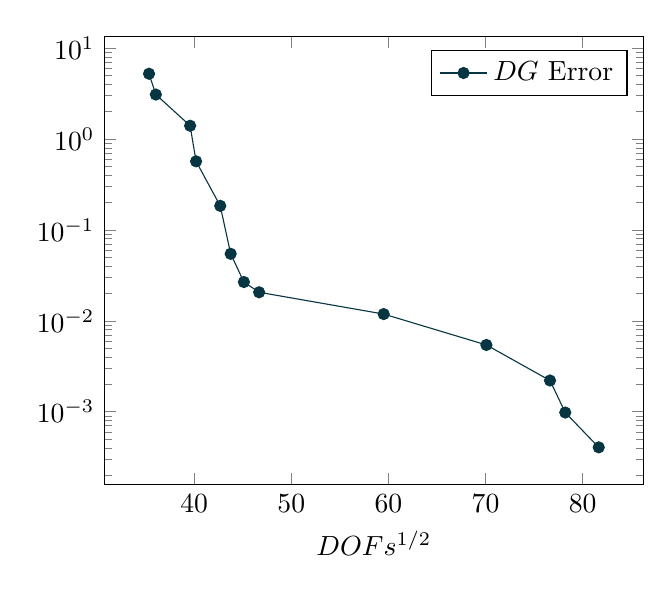
\begin{tikzpicture}
\begin{axis}[
    xlabel={$DOFs^{1/2}$}, % Edit if needed.
    legend pos=north east,
    ymode=log
]

\addplot[solarized-base02, mark=*] coordinates {(35.35533905932738,5.22824) (36.05551275463989,3.08808) (39.585350825778974,1.40074) (40.19950248448356,0.568479) (42.68489194082609,0.184123) (43.76071297408213,0.0545945) (45.12205669071391,0.0267047) (46.69047011971501,0.0206007) (59.51470406546604,0.0118629) (70.08566187174092,0.00542351) (76.6355009117837,0.0022026) (78.20485918406861,0.000978576) (81.65169930871004,0.000405115)};
\addlegendentry{$DG$ Error}

\end{axis}
\end{tikzpicture}
	\end{subfigure}
    \caption{$DG$ error versus $DOFs^{1/2}$ on a sequence of \textit{hp-adaptively} refined meshes over a square domain. $k_0 = 3$, $N_0 = 25$ (left) and $N_0 = 125$ (right).}
\end{figure}

\begin{figure}[!ht]
    \begin{subfigure}[b]{0.45\textwidth}
		% HP v DOFs template for TikZ.

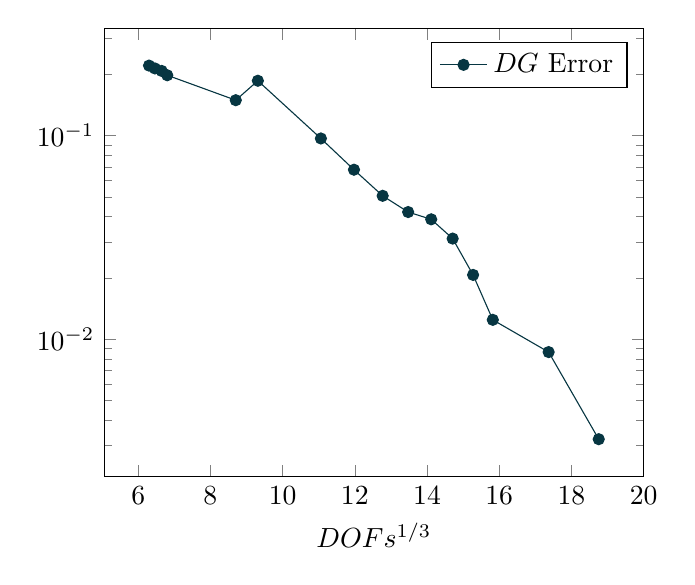
\begin{tikzpicture}
\begin{axis}[
    xlabel={$DOFs^{1/3}$}, % Edit if needed.
    legend pos=north east,
    ymode=log
]

\addplot[solarized-base02, mark=*] coordinates {(6.299605249474365,0.220458) (6.46330407009565,0.213463) (6.649399761150975,0.20759) (6.804092115953367,0.197661) (8.702188201949959,0.149058) (9.31401901560767,0.185737) (11.060275175811077,0.0966916) (11.976807054671553,0.0679165) (12.771142672954005,0.050558) (13.477328201610664,0.0420778) (14.116376860121461,0.0387551) (14.709984424285784,0.0311701) (15.276358607079842,0.0206684) (15.822251402102664,0.0124348) (17.369091205434305,0.00863551) (18.756827143467223,0.00322445)};
\addlegendentry{$DG$ Error}

\end{axis}
\end{tikzpicture}
	\end{subfigure}
	\hfill
	\begin{subfigure}[b]{0.45\textwidth}
		% HP v DOFs template for TikZ.

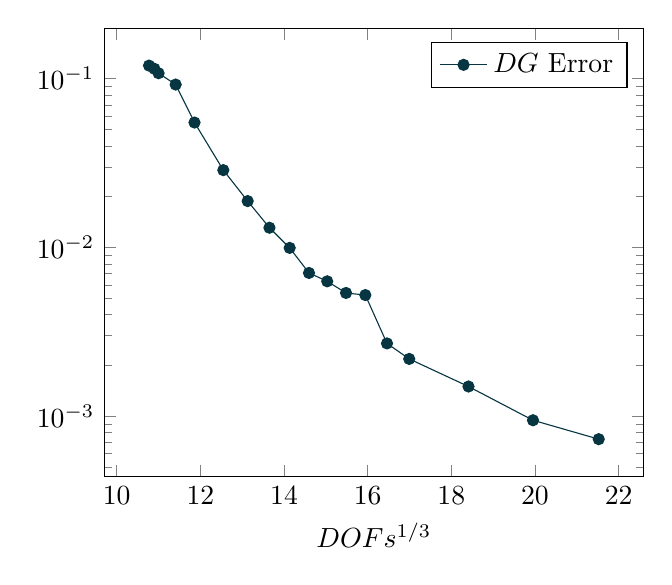
\begin{tikzpicture}
\begin{axis}[
    xlabel={$DOFs^{1/3}$}, % Edit if needed.
    legend pos=north east,
    ymode=log
]

\addplot[solarized-base02, mark=*] coordinates {(10.772173450159418,0.119546) (10.899918636993316,0.114459) (10.999999999999998,0.107735) (11.408857382284173,0.0922831) (11.859471855163267,0.054963) (12.548610714822335,0.0287119) (13.130828854692274,0.0188226) (13.651248393114228,0.0130834) (14.134753229443907,0.00993888) (14.596659021604594,0.00705952) (15.032522029472554,0.00629695) (15.482116036543895,0.00537315) (15.943813338821663,0.0052198) (16.46180328837959,0.00269895) (16.993076765677035,0.00218449) (18.410328165031775,0.00149923) (19.952386738818262,0.000945982) (21.524220046443375,0.000730821)};
\addlegendentry{$DG$ Error}

\end{axis}
\end{tikzpicture}
	\end{subfigure}
    \caption{$DG$ error versus $DOFs^{1/3}$ on a sequence of \textit{hp-adaptively} refined meshes over an L-shaped domain. $k_0 = 3$, $N_0 = 25$ (left) and $N_0 = 125$ (right).}
\end{figure}

\newpage
\subsubsection{Meshes}

\begin{figure}[!ht]
	\centering
    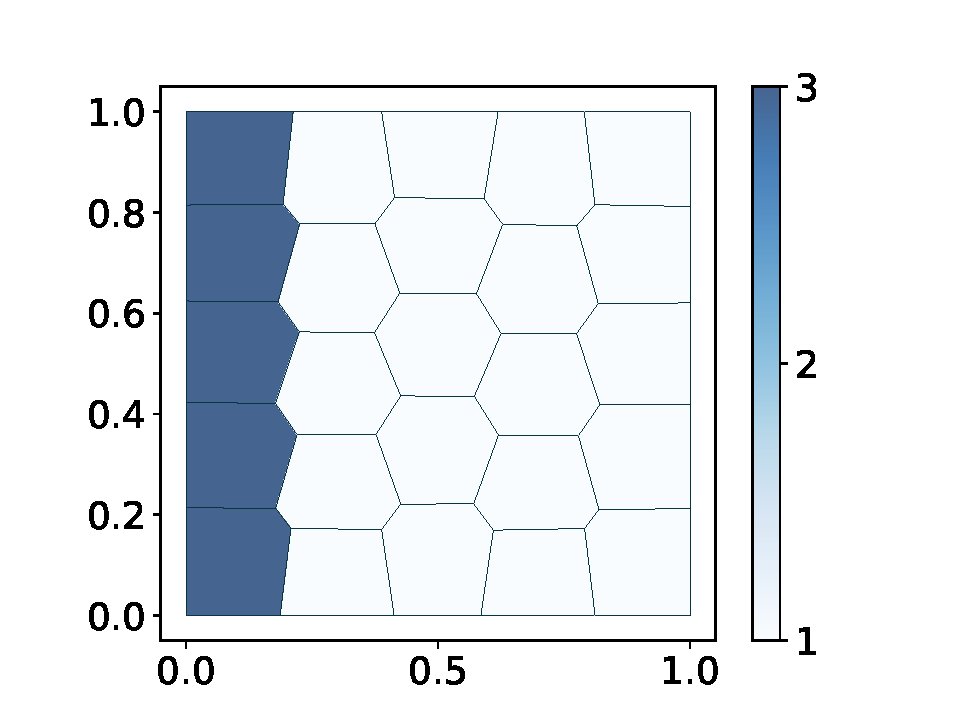
\includegraphics[trim=1cm 0.5cm 1cm 0.5cm, clip, width=0.3\textwidth]{meshes/adaptive/square_hp_1_2.pdf}
	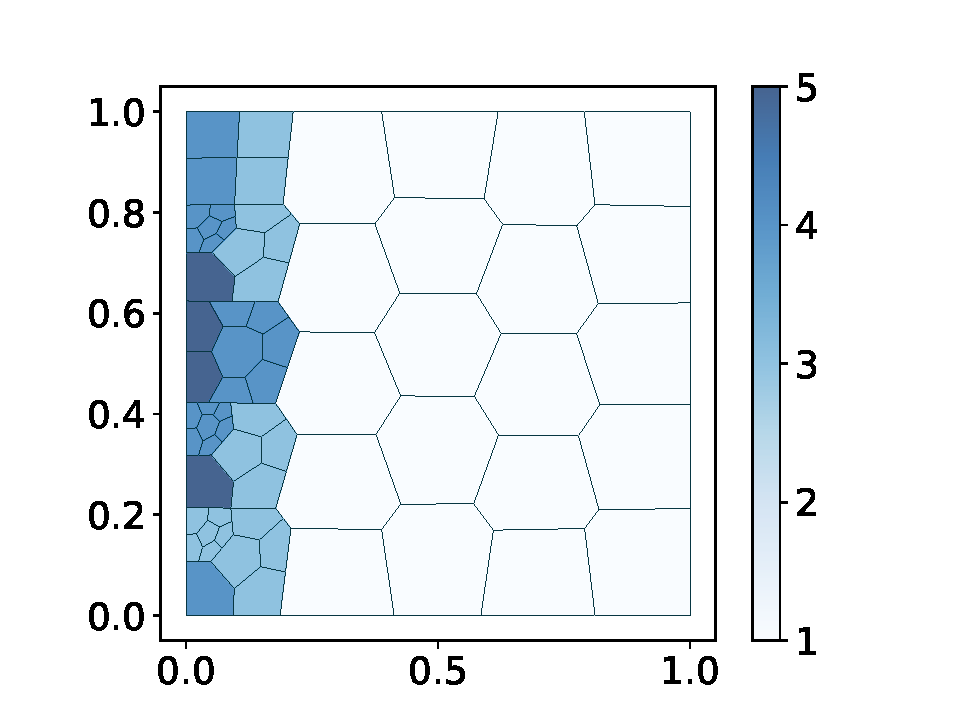
\includegraphics[trim=1cm 0.5cm 1cm 0.5cm, clip, width=0.3\textwidth]{meshes/adaptive/square_hp_1_5.pdf}
	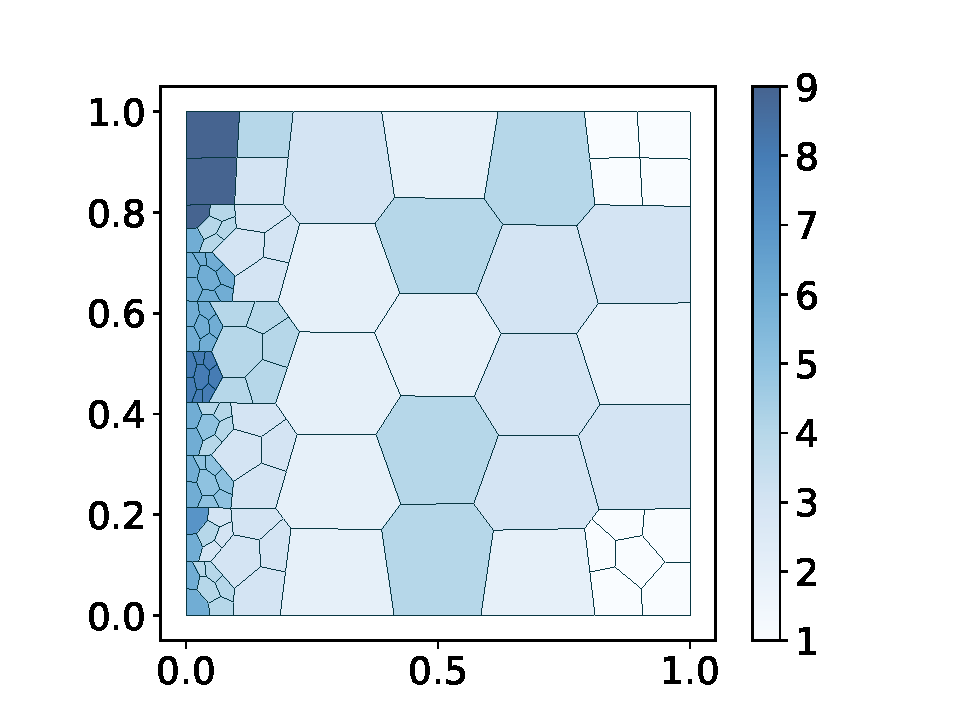
\includegraphics[trim=1cm 0.5cm 1cm 0.5cm, clip, width=0.3\textwidth]{meshes/adaptive/square_hp_1_10.pdf}
    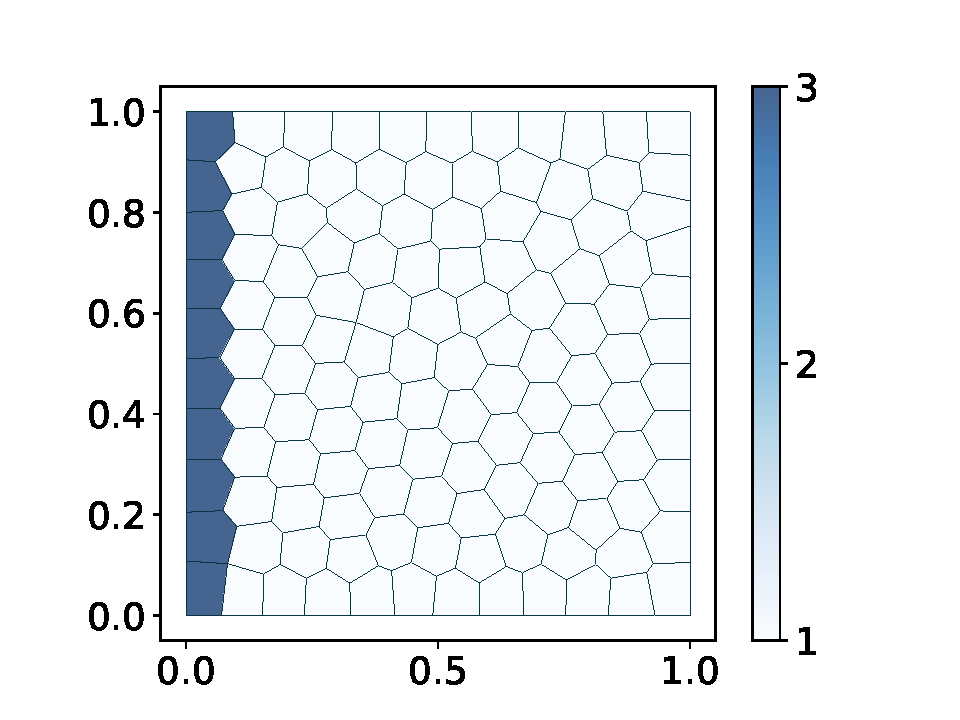
\includegraphics[trim=1cm 0.5cm 1cm 0.5cm, clip, width=0.3\textwidth]{meshes/adaptive/square_hp_125_1_2.pdf}
	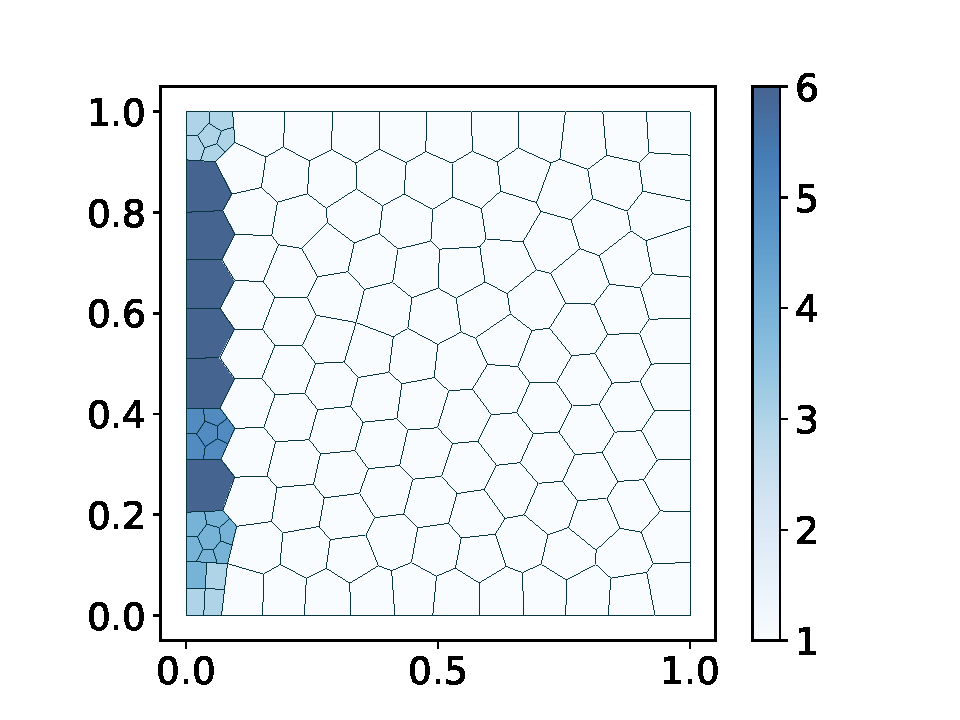
\includegraphics[trim=1cm 0.5cm 1cm 0.5cm, clip, width=0.3\textwidth]{meshes/adaptive/square_hp_125_1_5.pdf}
	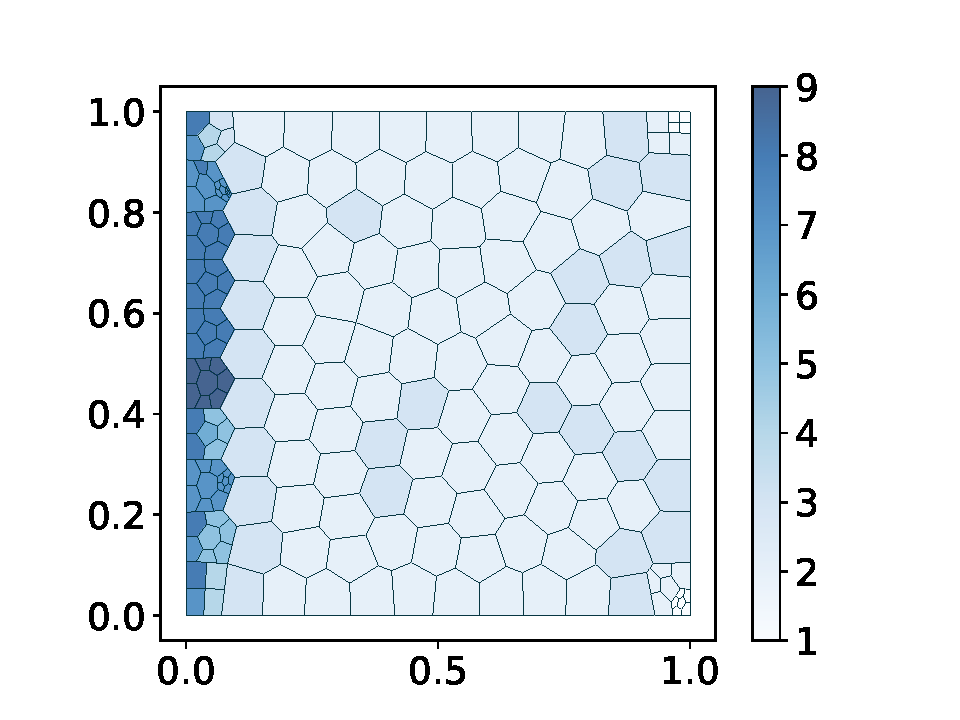
\includegraphics[trim=1cm 0.5cm 1cm 0.5cm, clip, width=0.3\textwidth]{meshes/adaptive/square_hp_125_1_10.pdf}
    \caption{Square mesh after 2, 5, and 10 refinements. $k_0 = 1$, $N_0 = 25$ (top) and $N_0 = 125$ (bottom).}
\end{figure}

\begin{figure}[!ht]
	\centering
	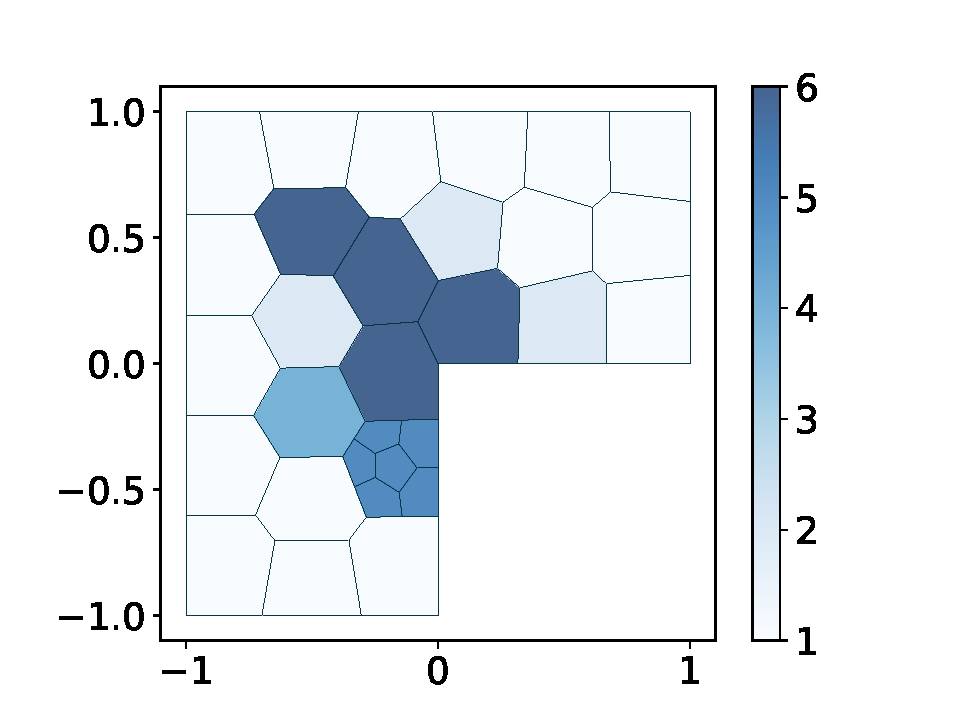
\includegraphics[trim=1cm 0.5cm 1cm 0.5cm, clip, width=0.3\textwidth]{meshes/adaptive/lshape_hp_1_5.pdf}
	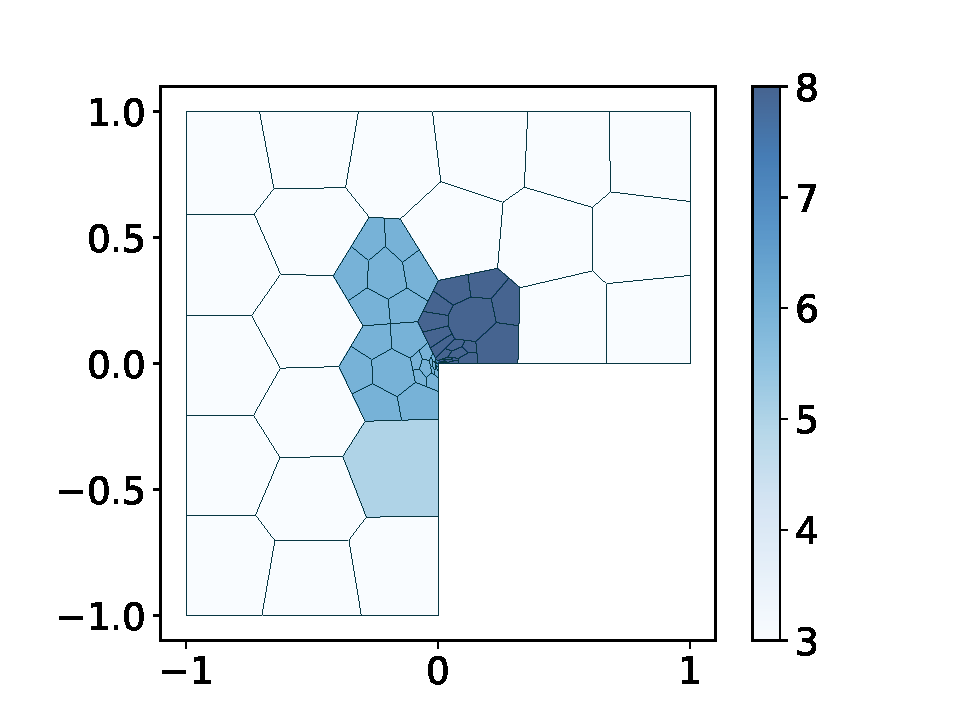
\includegraphics[trim=1cm 0.5cm 1cm 0.5cm, clip, width=0.3\textwidth]{meshes/adaptive/lshape_hp_1_10.pdf}
	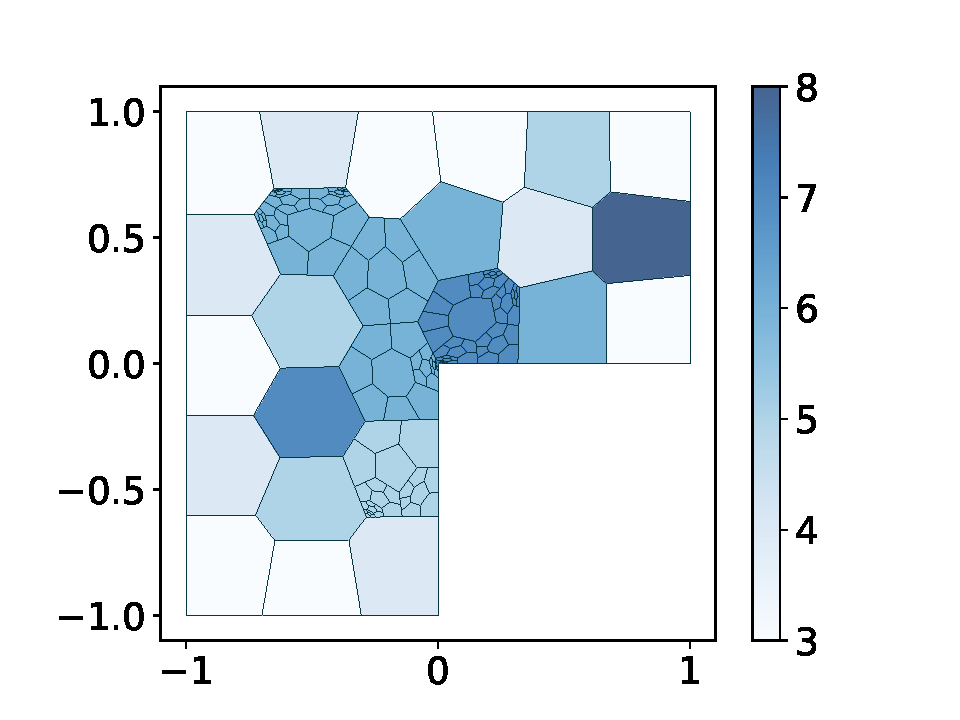
\includegraphics[trim=1cm 0.5cm 1cm 0.5cm, clip, width=0.3\textwidth]{meshes/adaptive/lshape_hp_1_15.pdf}
    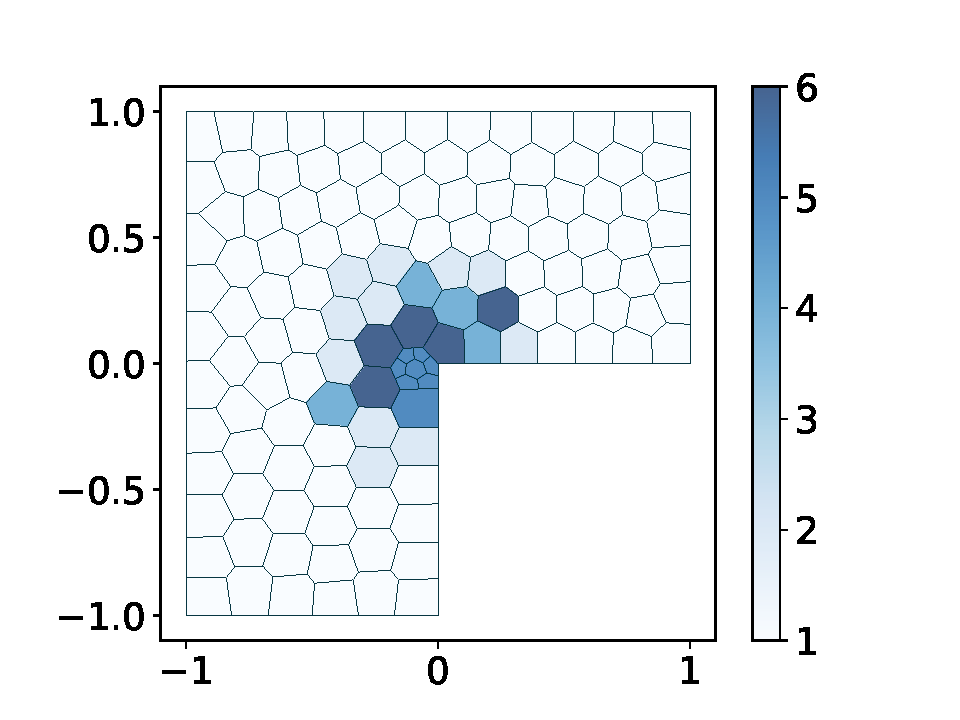
\includegraphics[trim=1cm 0.5cm 1cm 0.5cm, clip, width=0.3\textwidth]{meshes/adaptive/lshape_hp_125_1_5.pdf}
	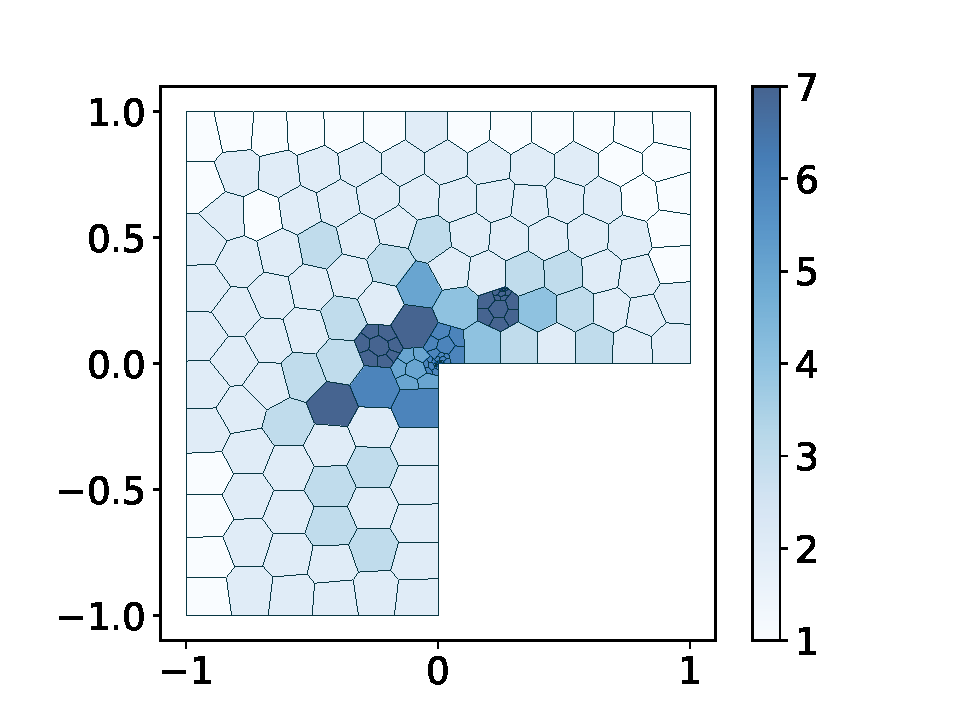
\includegraphics[trim=1cm 0.5cm 1cm 0.5cm, clip, width=0.3\textwidth]{meshes/adaptive/lshape_hp_125_1_10.pdf}
	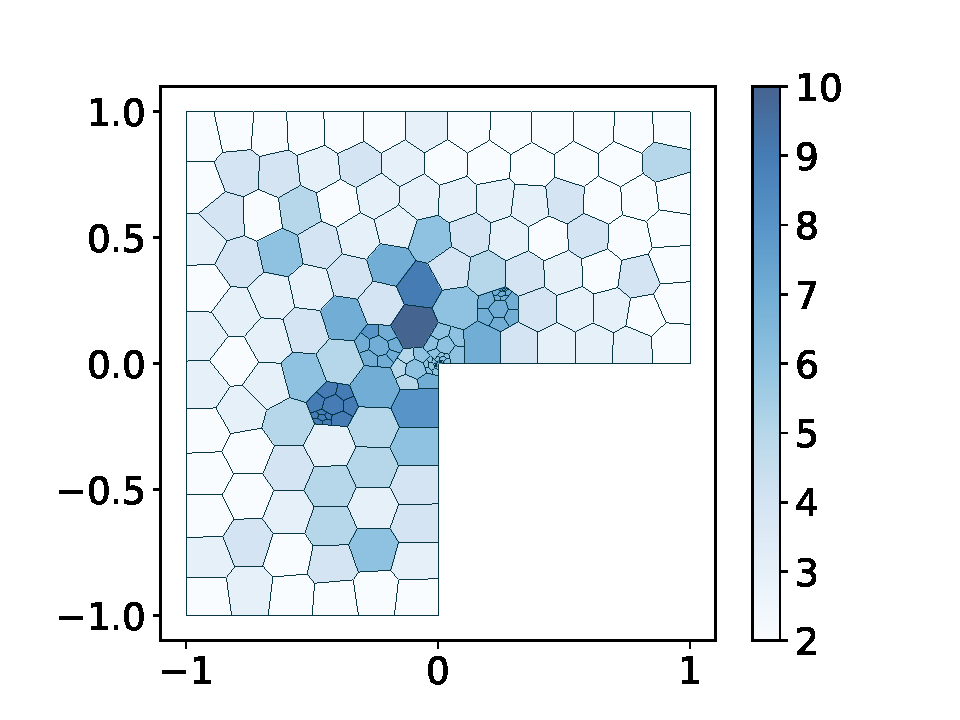
\includegraphics[trim=1cm 0.5cm 1cm 0.5cm, clip, width=0.3\textwidth]{meshes/adaptive/lshape_hp_125_1_15.pdf}
    \caption{L-shaped mesh after 5, 10, and 15 refinements. $k_0 = 1$, $N_0 = 25$ (top) and $N_0 = 125$ (bottom).}
\end{figure}

\newpage

\begin{figure}[!ht]
	\centering
    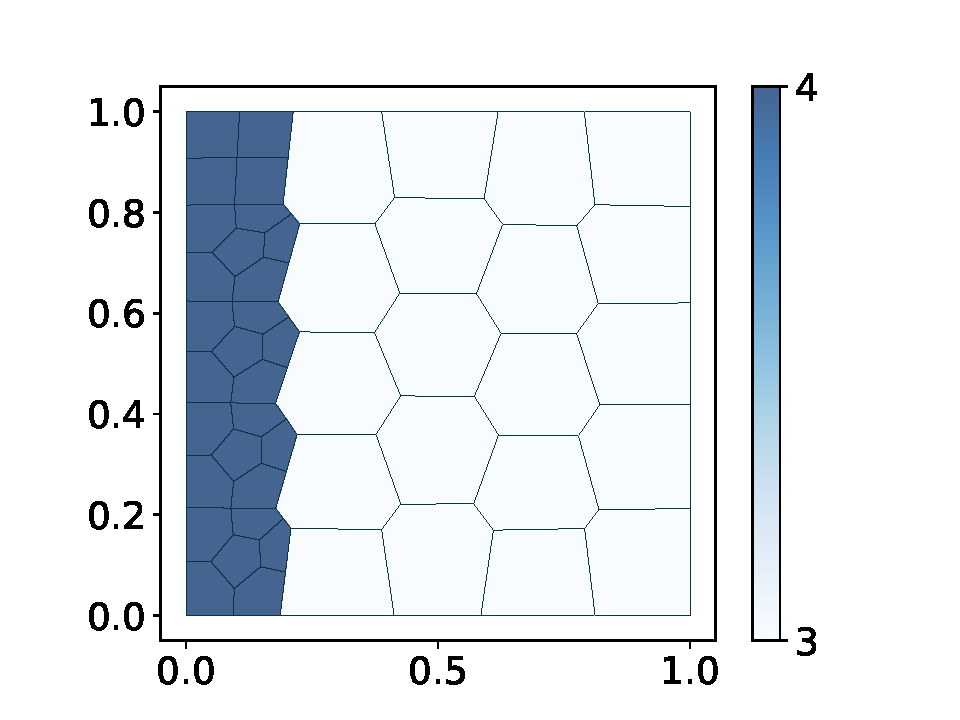
\includegraphics[trim=1cm 0.5cm 1cm 0.5cm, clip, width=0.3\textwidth]{meshes/adaptive/square_hp_2.pdf}
	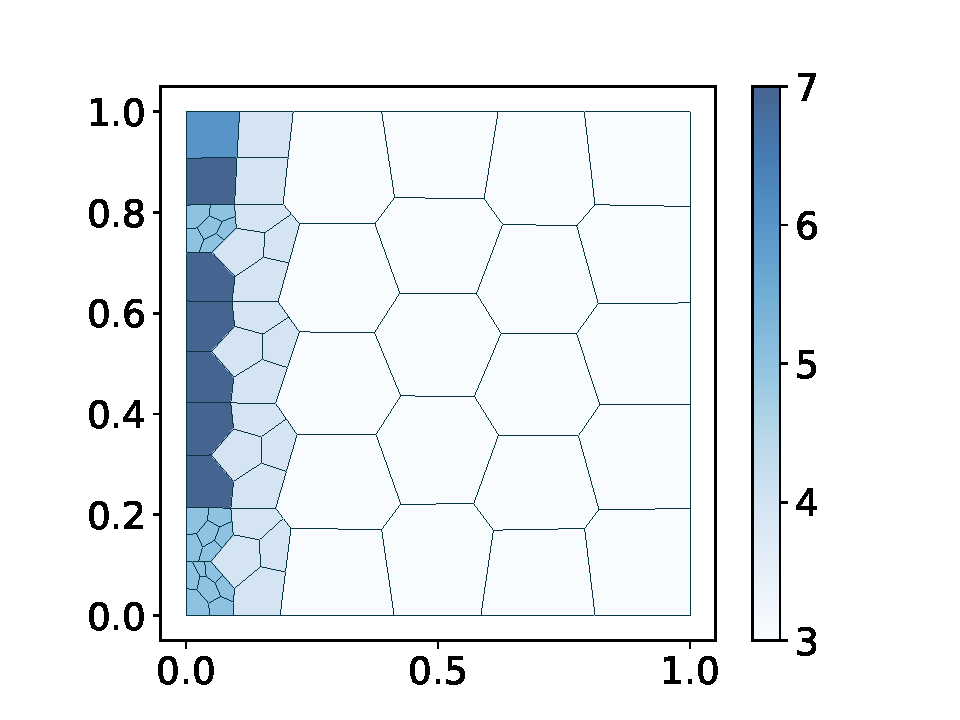
\includegraphics[trim=1cm 0.5cm 1cm 0.5cm, clip, width=0.3\textwidth]{meshes/adaptive/square_hp_5.pdf}
	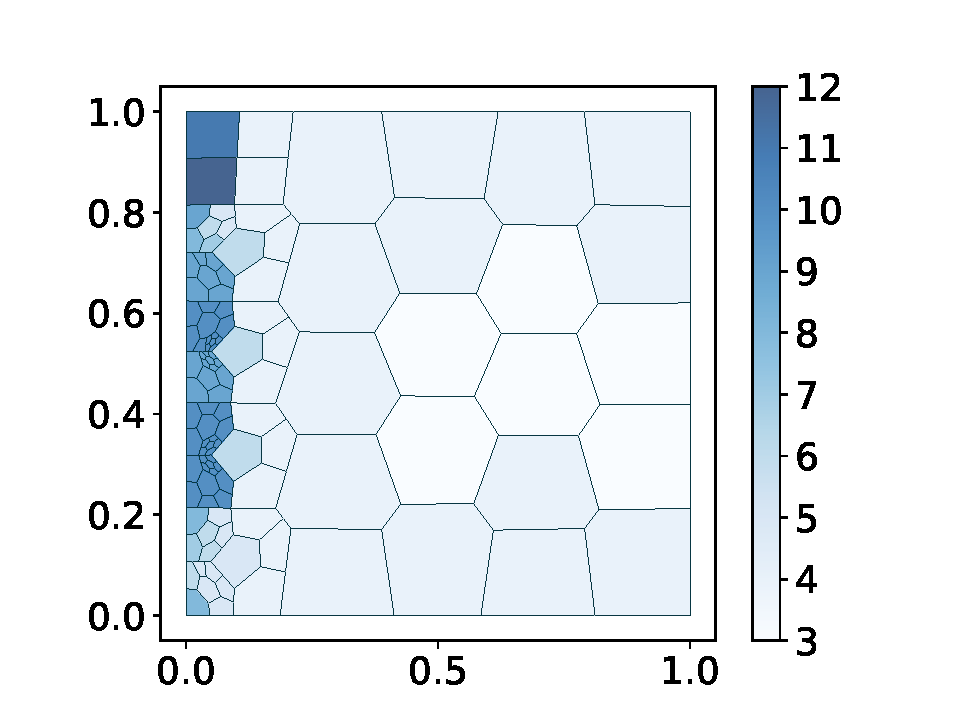
\includegraphics[trim=1cm 0.5cm 1cm 0.5cm, clip, width=0.3\textwidth]{meshes/adaptive/square_hp_10.pdf}
    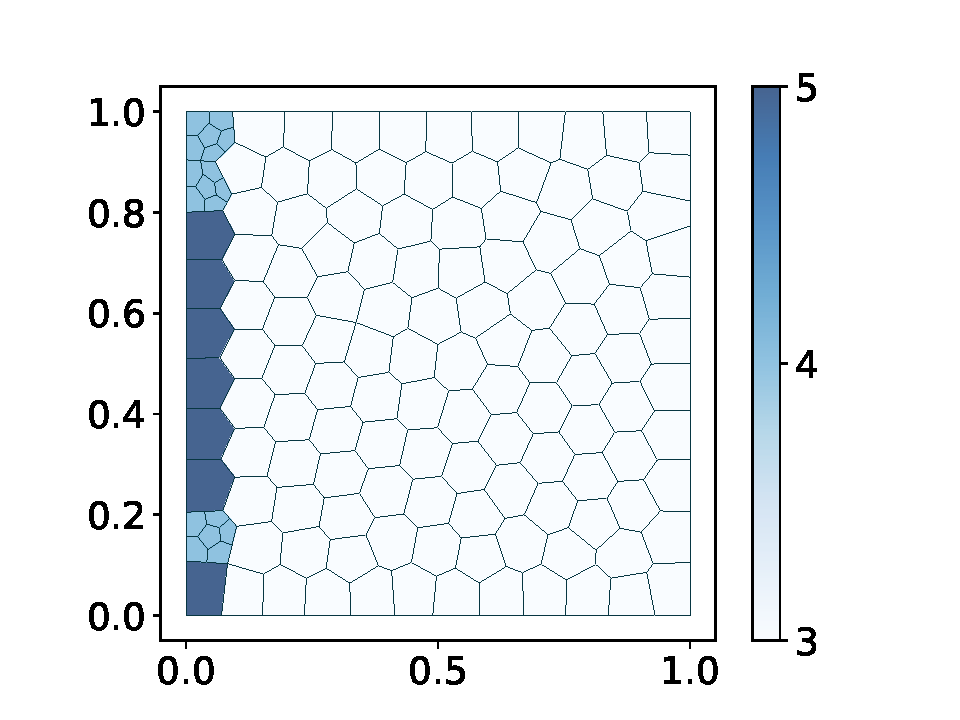
\includegraphics[trim=1cm 0.5cm 1cm 0.5cm, clip, width=0.3\textwidth]{meshes/adaptive/square_hp_125_2.pdf}
	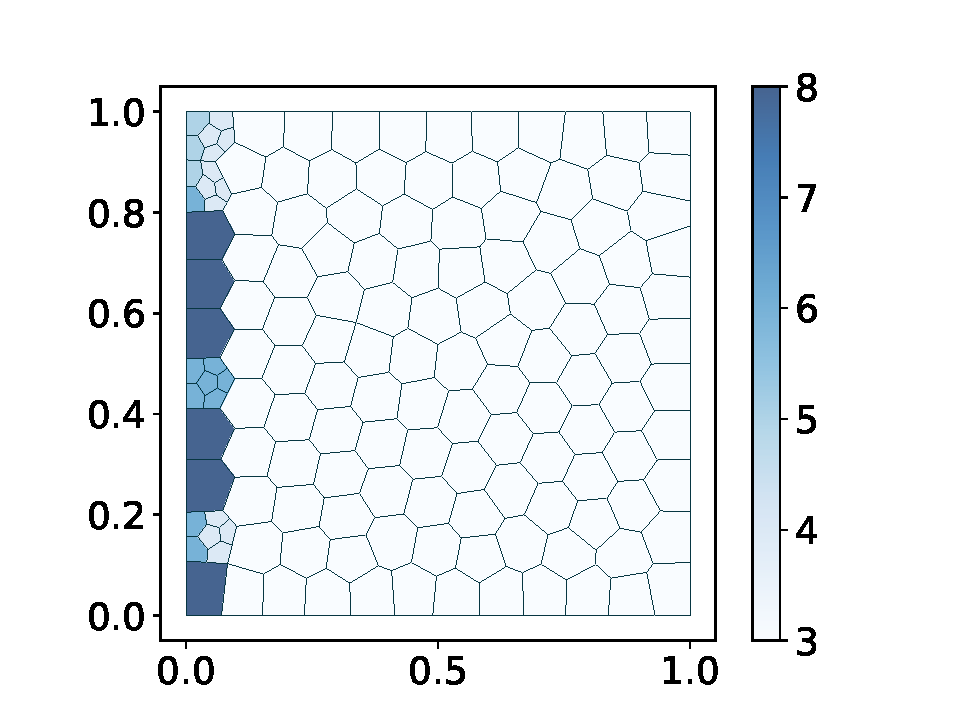
\includegraphics[trim=1cm 0.5cm 1cm 0.5cm, clip, width=0.3\textwidth]{meshes/adaptive/square_hp_125_5.pdf}
	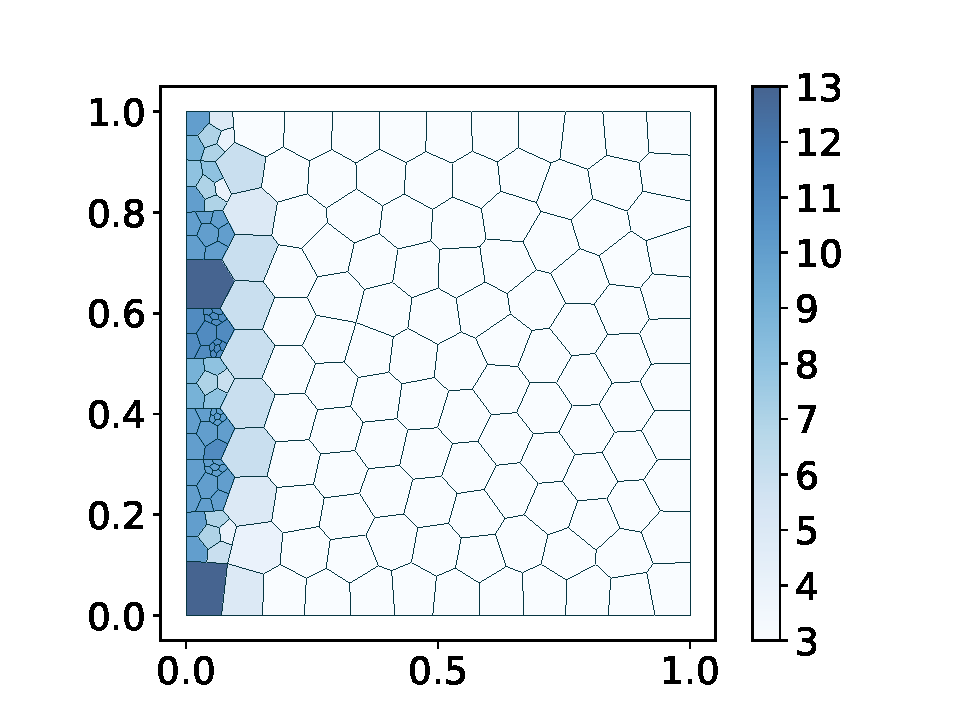
\includegraphics[trim=1cm 0.5cm 1cm 0.5cm, clip, width=0.3\textwidth]{meshes/adaptive/square_hp_125_10.pdf}
	\caption{Square mesh after 2, 5, and 10 refinements. $k_0 = 3$, $N_0 = 25$ (top) and $N_0 = 125$ (bottom).}
\end{figure}

\begin{figure}[!ht]
	\centering
	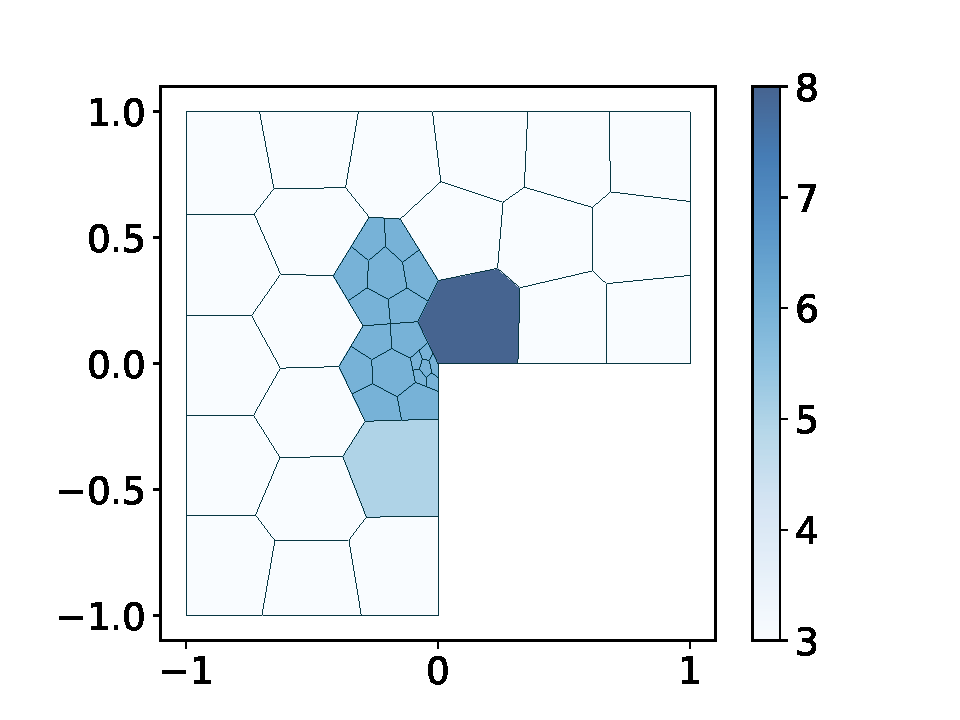
\includegraphics[trim=1cm 0.5cm 1cm 0.5cm, clip, width=0.3\textwidth]{meshes/adaptive/lshape_hp_5.pdf}
	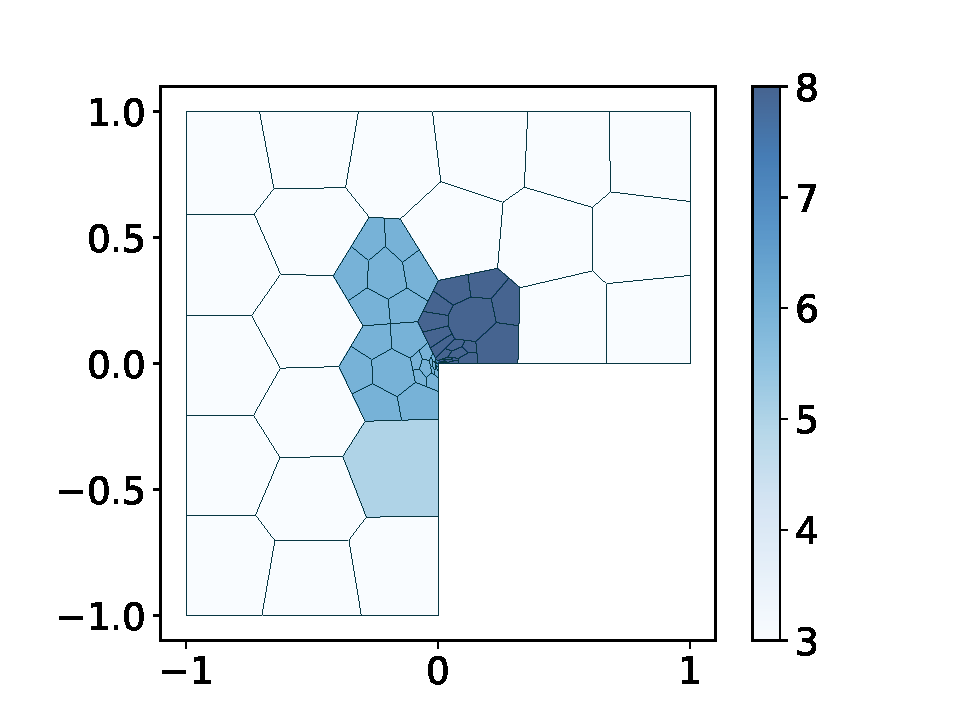
\includegraphics[trim=1cm 0.5cm 1cm 0.5cm, clip, width=0.3\textwidth]{meshes/adaptive/lshape_hp_10.pdf}
	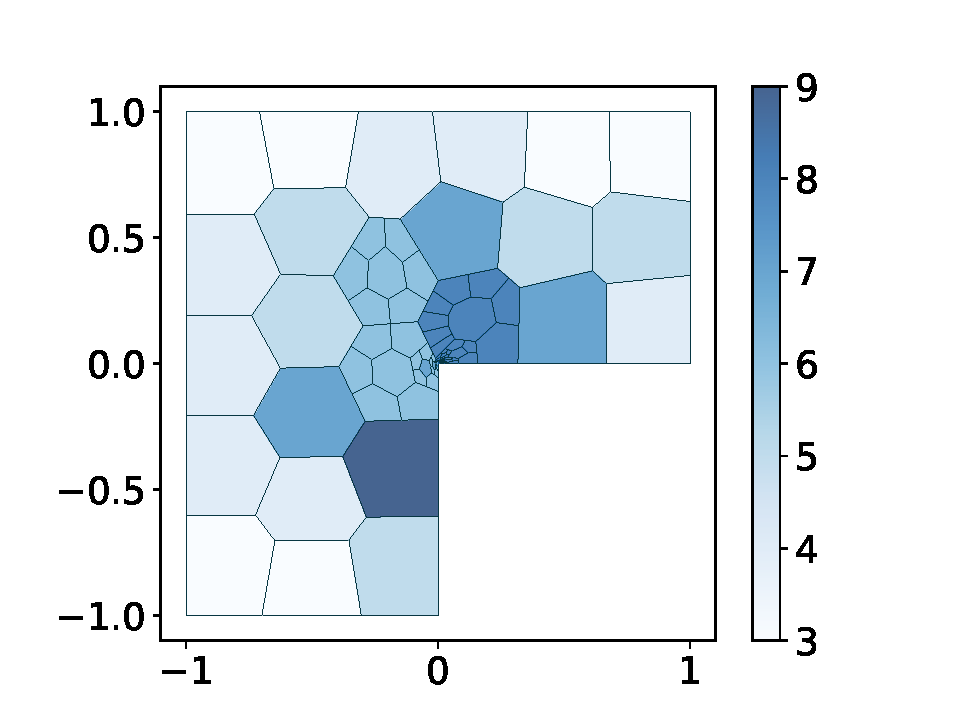
\includegraphics[trim=1cm 0.5cm 1cm 0.5cm, clip, width=0.3\textwidth]{meshes/adaptive/lshape_hp_15.pdf}
    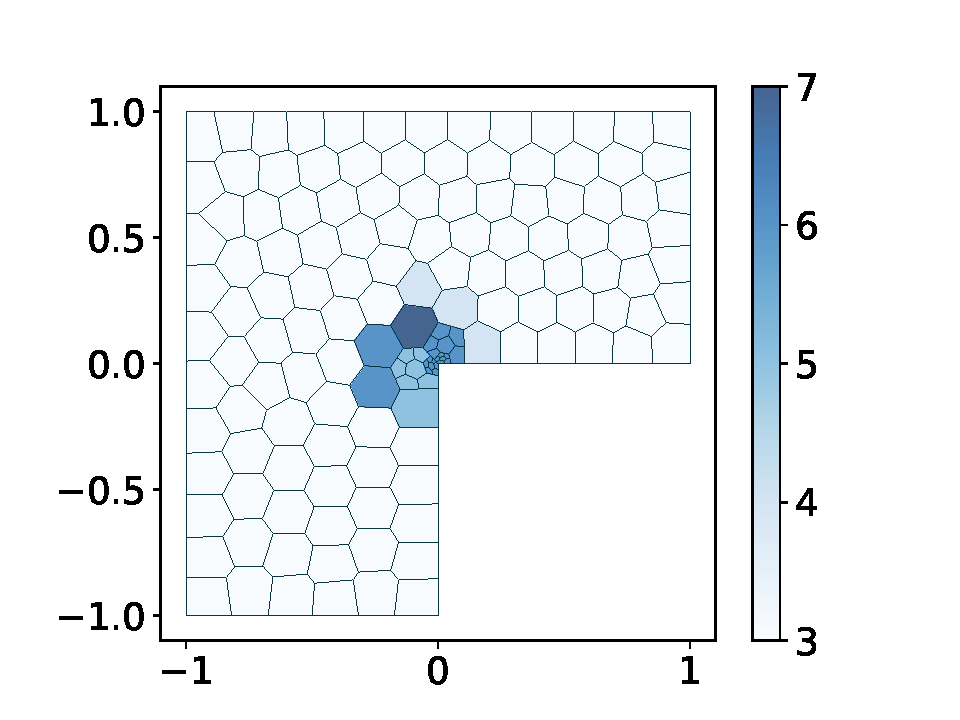
\includegraphics[trim=1cm 0.5cm 1cm 0.5cm, clip, width=0.3\textwidth]{meshes/adaptive/lshape_hp_125_5.pdf}
	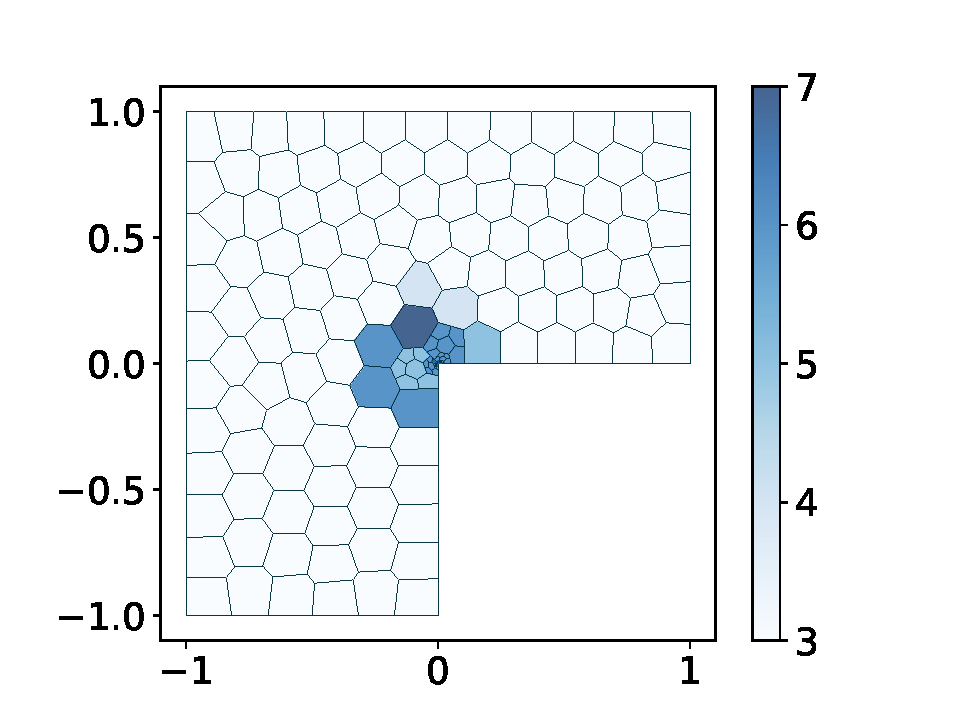
\includegraphics[trim=1cm 0.5cm 1cm 0.5cm, clip, width=0.3\textwidth]{meshes/adaptive/lshape_hp_125_10.pdf}
	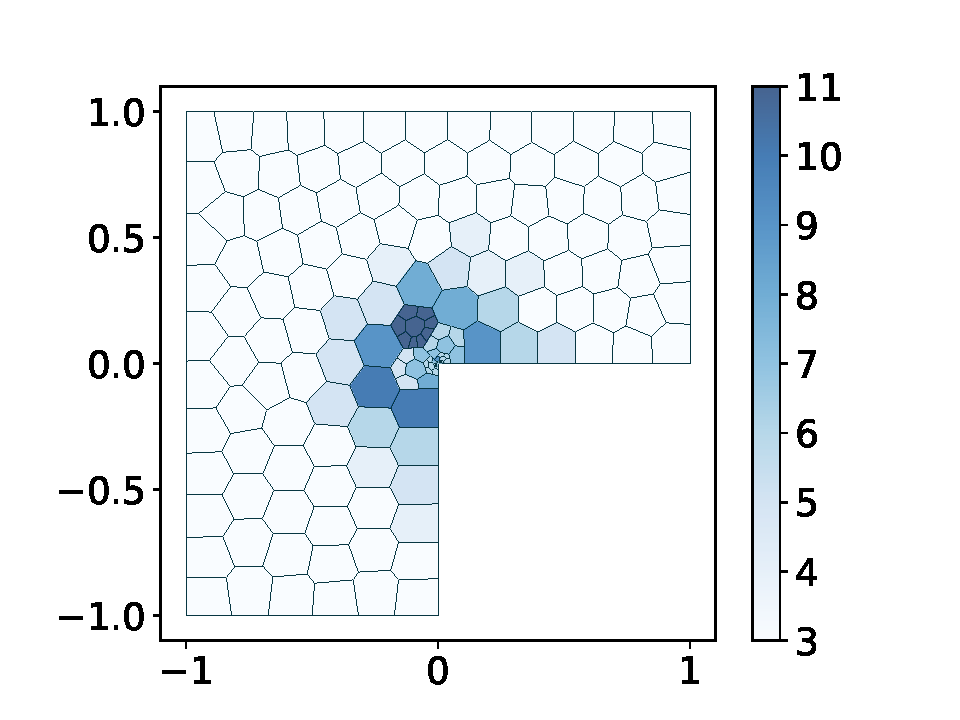
\includegraphics[trim=1cm 0.5cm 1cm 0.5cm, clip, width=0.3\textwidth]{meshes/adaptive/lshape_hp_125_15.pdf}
	\caption{L-shaped mesh after 5, 10, and 15 refinements. $k_0 = 3$, $N_0 = 25$ (top) and $N_0 = 125$ (bottom).}
\end{figure}

\newpage
\subsection{\textit{h-refinement} versus \textit{hp-refinement}}

The final step in implementing \textit{hp-adaptivity} is to compare the results of \textit{h-refinement} and \textit{hp-refinement}. One approach is to choose a basic starting mesh, using a low polynomial degree and a small number of elements.

\begin{figure}[!ht]
    \begin{subfigure}[b]{0.45\textwidth}
		% HP v DOFs template for TikZ.

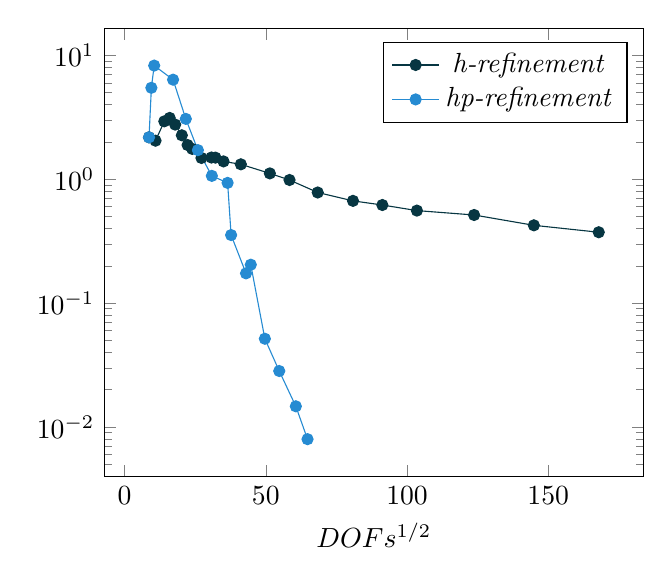
\begin{tikzpicture}
\begin{axis}[
    xlabel={$DOFs^{1/2}$}, % Edit if needed.
    legend pos=north east,
    ymode=log
]

\addplot[solarized-base02, mark=*] coordinates {(8.660254037844387,2.1812) (10.954451150103322,2.04967) (14.071247279470288,2.93871) (15.968719422671311,3.13011) (17.916472867168917,2.76594) (20.273134932713294,2.26584) (22.315913604421397,1.89116) (23.93741840717165,1.76002) (27.2213151776324,1.48665) (30.740852297878796,1.49861) (32.17141588429082,1.49545) (35.02855977627399,1.39444) (41.1703777004778,1.3207) (51.43928459844674,1.11561) (58.40376700179535,0.986776) (68.38859554048467,0.782051) (80.87026647662292,0.669326) (91.27431182978046,0.619557) (103.50362312499017,0.558376) (123.75378782081783,0.514557) (144.9137674618944,0.424657) (167.88388844674762,0.373345)};
\addlegendentry{\textit{h-refinement}}

\addplot[\accentcolor, mark=*] coordinates {(8.660254037844387,2.1812) (9.486832980505138,5.48286) (10.488088481701515,8.28706) (17.175564037317667,6.37634) (21.6794833886788,3.07509) (25.96150997149434,1.71936) (30.903074280724887,1.06513) (36.4828726939094,0.935197) (37.72267222772003,0.3543) (43.0,0.173769) (44.68780594300866,0.204124) (49.66890375275057,0.0514923) (54.76312628037227,0.0282501) (60.63827174318213,0.0146515) (64.77653896280658,0.0079507)};
\addlegendentry{\textit{hp-refinement}}

\end{axis}
\end{tikzpicture}
	\end{subfigure}
	\hfill
	\begin{subfigure}[b]{0.45\textwidth}
		% HP v DOFs template for TikZ.

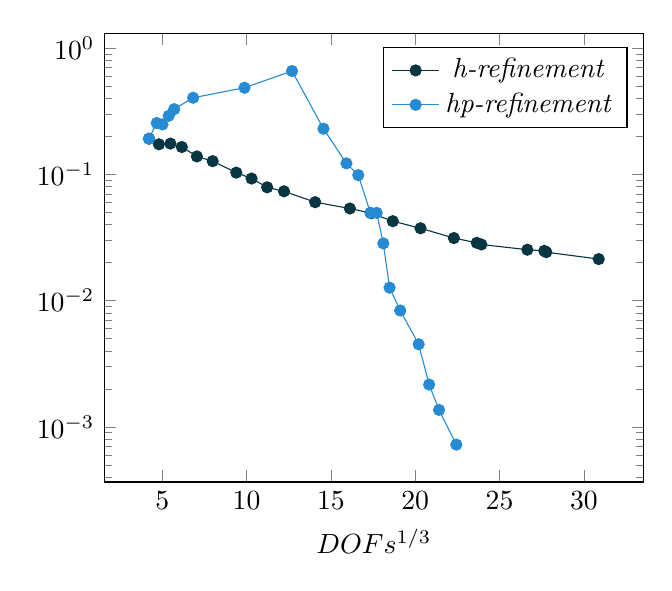
\begin{tikzpicture}
\begin{axis}[
    xlabel={$DOFs^{1/3}$}, % Edit if needed.
    legend pos=north east,
    ymode=log
]

\addplot[solarized-base02, mark=*] coordinates {(4.217163326508746,0.191755) (4.805895533705332,0.173165) (5.484806552432618,0.17539) (6.162240147749038,0.164783) (7.054004063162272,0.138814) (7.989569740454012,0.127309) (9.39024187300355,0.103252) (10.297715269155368,0.0927241) (11.221408880627516,0.0789875) (12.21822948857921,0.073464) (14.067699311995325,0.0602545) (16.126599805218184,0.0536889) (17.386751706878687,0.0492177) (18.66925275961817,0.0425939) (20.31339680458661,0.0374376) (22.29090233304798,0.0313125) (23.651205489315725,0.028713) (23.918123773897065,0.0278557) (26.648390254618004,0.0253127) (27.653467034596552,0.0247917) (27.769363970258176,0.0242055) (30.87951848068366,0.0213387)};
\addlegendentry{\textit{h-refinement}}

\addplot[\accentcolor, mark=*] coordinates {(4.217163326508746,0.191755) (4.672328728355259,0.255398) (5.0132979349645845,0.248801) (5.383212612087283,0.291174) (5.708267473384861,0.328607) (6.832771452246442,0.404871) (9.878530490026034,0.485699) (12.69507321245234,0.659013) (14.55901434377428,0.230073) (15.921490395218942,0.122269) (16.623800957486996,0.098664) (17.340316055801914,0.0495985) (17.714635665253457,0.0495794) (18.10839938601742,0.0283923) (18.477938151928672,0.0126687) (19.10925056502305,0.00835058) (20.20211721754757,0.00451385) (20.823924640400417,0.00216312) (21.4106622851008,0.00136207) (22.436197851201577,0.00072339)};
\addlegendentry{\textit{hp-refinement}}

\end{axis}
\end{tikzpicture}
	\end{subfigure}
    \caption{$DG$ error versus $DOFs^{1/2}$ (left) and $DOFs^{1/3}$ (right) on sequences of \textit{h-adaptively} (black) and \textit{hp-adaptively} (blue) refined meshes over a square (left) and an L-shaped domain (right). $k_0 = 1$, $N_0 = 25$.}
\end{figure}

This comparison highlights the superiority of the \textit{hp-adaptive} method over the \textit{h-adaptive} approach, greatly reducing the error while utilizing significantly fewer $DOFs$.

\newpage
\subsection{A code snippet}

Here's a snippet to illustrate the \textit{hp-adaptive} mesh refinement from the user's perspective:

\lstinputlisting[style=cpp, firstline=11]{../snippets/hp_refine.cpp}

	\newpage
    \section{Conclusion}
	This report has provided a comprehensive study of adaptive mesh refinement strategies within the context of the Discontinuous Galerkin (DG) method, focusing on both \textit{h-adaptivity} and \textit{p-adaptivity}.

The evaluation of \textit{h-adaptive} refinement strategies demonstrated their effectiveness in managing complex geometries and solutions with local singularities. This approach effectively reduces local discretization errors by refining the mesh where needed.

In the domain of \textit{p-adaptivity}, the analysis of the decay rates of Legendre coefficients proved to be a reliable method for assessing solution smoothness and guiding polynomial order adjustments.

A comparison of \textit{h-adaptive} and \textit{hp-adaptive} refinement strategies highlighted their respective advantages. While \textit{h-adaptivity} effectively manages local errors through mesh refinement, \textit{hp-adaptivity} offers additional benefits by adjusting polynomial orders alongside mesh resolution.

Overall, the results of this project underscore the practical benefits of adaptive refinement strategies in DG methods. By utilizing a posteriori error estimators, \textit{h-adaptivity} and \textit{hp-adaptivity} can be effectively implemented to achieve accurate and efficient numerical solutions.

	\newpage
	\addcontentsline{toc}{section}{References}
	\printbibliography

	\newpage
	
	\vspace*{\fill}
	\begin{center}
		Compiled on \today.
	\end{center}
	\vspace*{\fill}

	\thispagestyle{empty}

\end{document}
